%% ----------------------------------------------------------------
%% Thesis.tex -- MAIN FILE (the one that you compile with LaTeX)
%% ----------------------------------------------------------------

% Set up the document
%\documentclass[a4paper, 11pt, oneside]{Thesis}  % Use the "Thesis" style, based on the ECS Thesis style by Steve Gunn
%\documentclass[a4paper, 11pt, twoside, openright]{Thesis} %en a4
\documentclass[a4paper, 12pt, twoside, openright]{Thesis} %para reducir a b5
\graphicspath{{Figures/}}  % Location of the graphics files (set up for graphics to be in PDF format)

% Include any extra LaTeX packages required
\usepackage[square, numbers, comma, sort&compress]{natbib}  % Use the "Natbib" style for the references in the Bibliography
\usepackage{verbatim}  % Needed for the "comment" environment to make LaTeX comments
\usepackage{vector}  % Allows "\bvec{}" and "\buvec{}" for "blackboard" style bold vectors in maths
\usepackage{mathtools}

\usepackage{parskip} %para que haga el indent al principio de cada parrafo
\setlength{\parindent}{15pt}
\usepackage{indentfirst} %para que ponga el indent en el primer parrafo tambien, sino no lo hace

\hypersetup{urlcolor=blue, colorlinks=true}  % Colours hyperlinks in blue, but this can be distracting if there are many links.

%% ----------------------------------------------------------------
\begin{document}

%Abreviaciones de comandos y nuevos comandos.
\def\la{\langle}
\def\ra{\rangle}
\def\beq{\begin{equation}}
\def\eeq{\end{equation}}
\def\beqa{\begin{eqnarray}}
\def\eeqa{\end{eqnarray}}
\def\blankpage{
\newpage
\begin{equation}
\nonumber
\end{equation}
\newpage}
\def\ssst{\scriptscriptstyle}   %%para hacer más pequeñas algunas ecuaciones

\newcommand{\beqas}{\begin{eqnarray*}}
\newcommand{\eeqas}{\end{eqnarray*}}
\newcommand {\fexp} [1] {\exp \left( #1 \right)}
\newcommand {\fabs}[1] {\left| #1 \right|}
\newcommand{\cR}{{\cal{R}}}
\newcommand{\new}[1]{{\it #1}}

\frontmatter	  % Begin Roman style (i, ii, iii, iv...) page numbering

% Set up the Title Page
%----------------------------------------------------------------------------------------------------------------------------------------------------------
%----------------------------------------------------------------------------------------------------------------------------------------------------------
%----------------------------------------------------------------------------------------------------------------------------------------------------------
\begin{titlepage}
\thispagestyle{empty} %\vspace*{0.1cm}
\hspace{-0.3cm}\includegraphics[scale=0.25]{ehu}\hspace{0.3cm}
\bigskip
{\centering \large
\par \vspace{1cm}

\hrule\vspace*{0.5cm}

{\LARGE \bf {Asymmetric Quantum Devices and Heat Transport}}

\vspace{0.7cm}\hrule \vspace{2.75cm}
{\LARGE \bf{Miguel \'{A}ngel Sim\'{o}n Mart\'{i}nez}}\\
\vspace{1.25cm}
{\it{Supervisors:}} \\
\vspace{0.1cm}
{\large \bf {Prof. Juan Gonzalo Muga Francisco}}\\
{\large \bf {Prof. Maria Luisa Pons Barba}}\\
\vspace{2.2cm}
\begin{figure}[h]
{\centering {

}\par}
\end{figure}
\vspace{1.0cm}
Departamento de Qu\'{\i}mica-F\'{\i}sica\\
Facultad de Ciencia y Tecnolog\'ia\\
Universidad del Pa\'is Vasco/Euskal Herriko Unibertsitatea\\ (UPV/EHU)\\
\vspace*{1.0cm}
\hspace{5.5cm}Leioa, Febrero 2021} \pagebreak
\end{titlepage}
%we use the title page document
%\newpage
%\mbox{}
%\thispagestyle{plain} % para que no se numere esta p�gina

%This is another way of generating a title page, (in fact below it is written how to use )
%\title  {Shortcuts to adiabaticity in the double well}
%\authors  {\texorpdfstring
%           {\href{sofia.martinez@ehu.eus}{Sof\'ia Mart\'inez Garaot}}
%            {}
%            }

%\addresses  {\groupname\\\deptname\\\univname}  % Do not change this here, instead these must be set in the "Thesis.cls" file, please look through it instead
%\date       {\today}
%\subject    {}
%\keywords   {}

%\maketitle
%----------------------------------------------------------------------------------------------------------------------------------------------------------
%----------------------------------------------------------------------------------------------------------------------------------------------------------
%----------------------------------------------------------------------------------------------------------------------------------------------------------

\setstretch{1.3}  % It is better to have smaller font and larger line spacing than the other way round

% Define the page headers using the FancyHdr package and set up for one-sided printing
\fancyhead{}  % Clears all page headers and footers
\rhead{\thepage}  % Sets the right side header to show the page number
\lhead{}  % Clears the left side page header

\pagestyle{fancy}  % Finally, use the "fancy" page style to implement the FancyHdr headers

\clearpage  % Declaration ended, now start a new page

%Meto una pagina en blanco
\pagestyle{empty}  % No headers or footers for the following pages
\null\vfill

\vfill\vfill\vfill\vfill\vfill\vfill\null
\clearpage  % Empty page ended, start a new page


%% ----------------------------------------------------------------
% The "Funny Quote Page"
\pagestyle{empty}  % No headers or footers for the following pages

\null\vfill
% Now comes the "Funny Quote", written in italics
\textit{``Insert deep/meaningful/clever quote by someone who you admire or hate''}

\begin{flushright}
Someone who you admire or hate
\end{flushright}

\vfill\vfill\vfill\vfill\vfill\vfill\null
\clearpage  % Funny Quote page ended, start a new page
%% ----------------------------------------------------------------

%% The Abstract Page
%\addtotoc{Abstract}  % Add the "Abstract" page entry to the Contents
%\abstract{
%\addtocontents{toc}{\vspace{1em}}  % Add a gap in the Contents, for aesthetics
%
%The Thesis Abstract is written here (and usually kept to just this page). The page is kept centered vertically so can expand into the blank space above the title too\ldots
%
%}
%
%\clearpage  % Abstract ended, start a new page
%%% ----------------------------------------------------------------

%Meto una pagina en blanco
\pagestyle{empty}  % No headers or footers for the following pages

\null\vfill

\vfill\vfill\vfill\vfill\vfill\vfill\null
\clearpage  % Empty page ended, start a new page

\setstretch{1.3}  % Reset the line-spacing to 1.3 for body text (if it has changed)

% The Acknowledgements page, for thanking everyone
\acknowledgements{
\addtocontents{toc}{\vspace{1em}}  % Add a gap in the Contents, for aesthetics
Do not forget about the people that has been by your side and supported you.
\it{Esta Tesis ha sido financiada a trav\'es de una beca predoctoral concedida por el Gobierno Vasco/Eusko Jaurlaritza}

}

\clearpage  % End of the Acknowledgements
%% ----------------------------------------------------------------

\pagestyle{fancy}  %The page style headers have been "empty" all this time, now use the "fancy" headers as defined before to bring them back


%% ----------------------------------------------------------------
\lhead{\emph{Contents}}  % Set the left side page header to "Contents"
\tableofcontents  % Write out the Table of Contents

%% ----------------------------------------------------------------
\lhead{\emph{List of Figures}}  % Set the left side page header to "List if Figures"
\listoffigures  % Write out the List of Figures

%%% ----------------------------------------------------------------
%\lhead{\emph{List of Tables}}  % Set the left side page header to "List of Tables"
%\listoftables  % Write out the List of Tables

%% ----------------------------------------------------------------
\setstretch{1.5}  % Set the line spacing to 1.5, this makes the following tables easier to read
\clearpage  % Start a new page

%% Begin the Dedication page
\setstretch{1.3}  % Return the line spacing back to 1.3
\pagestyle{empty}  % Page style needs to be empty for this page
\dedicatory{dedicatory here}

\addtocontents{toc}{\vspace{1em}}  % Add a gap in the Contents, for aesthetics
\chapter{List of publications} % Write in your own chapter title
\label{Publications}
\lhead{\emph{List of publications}} % Write in your own chapter title to set the page header
\hspace{-0.5 cm}{{\large\bf \rm I)}} {\bf The results of this Thesis are based on the following articles}
\section*{Published Articles}

\begin{enumerate}

  \item M. Pons, Y. Y. Cui, A. Ruschhaupt, {\bf M. A. Sim\'{o}n} and J. G. Muga\\
  {\it Local rectification of heat flux}\\
  \href{https://doi.org/10.1209/0295-5075/119/64001}{EPL {\bf 119}, 64001 (2017).}

  \item A. Ruschhaupt, T. Dowdall, {\bf M. A. Sim\'{o}n} and J. G. Muga\\
  {\it Asymmetric scattering by non-Hermitian potentials}\\
  \href{https://doi.org/10.1209/0295-5075/120/20001}{EPL {\bf 120}, 20001 (2017).}

  \item {\bf M. A. Sim\'{o}n}, A. Buend\'{i}a and J. G. Muga\\
  {\it Symmetries and Invariants for Non-Hermitian Hamiltonians}\\
  \href{https://doi.org/10.3390/math6070111}{Mathematics {\bf 6}, 111 (2018).}

  \item {\bf M. A. Sim\'{o}n}, A. Buend\'{i}a, A. Kiely, A. Mostafazadeh and J. G. Muga\\
  {\it $S$-matrix pole symmetries for non-Hermitian scattering Hamiltonians}\\
  \href{https://doi.org/10.1103/PhysRevA.99.052110}{Phys. Rev. A {\bf 99}, 052110 (2019).}

  \item {\bf M. A. Sim\'{o}n}, S. Mart\'{i}nez-Garaot, M. Pons and J. G. Muga\\
  {\it Asymmetric heat transport in ion crystals}\\
  \href{https://doi.org/10.1103/PhysRevE.100.032109}{Phys. Rev. E {\bf 100}, 032109 (2019).}

  \item A. Alaña, S. Mart\'{i}nez-Garaot, {\bf M. A. Sim\'{o}n} and J. G. Muga\\
  {\it Symmetries of (${N \times N}$ ) non-Hermitian Hamiltonian matrices}\\
  \href{https://doi.org/10.1088/1751-8121/ab7781}{J. Phys. A: Math. Theor. {\bf 53}, 135304 (2020).}

  \item A. Ruschhaupt, A. Kiely, {\bf M. A. Sim\'{o}n} and J. G. Muga\\
  {\it Quantum-optical implementation of non-Hermitian potentials for asymmetric scattering}\\
  \href{https://doi.org/10.1103/PhysRevA.102.053705}{Phys. Rev. A {\bf 102}, 053705 (2020).}\\

  \item {\bf M. A. Sim\'{o}n}, A. Alaña, M. Pons, A. Ruiz-Garc\'{i}a and J. G. Muga\\
  {\it Heat rectification with a minimal model of two harmonic oscillators}\\
  \href{https://doi.org/10.1103/PhysRevE.103.012134}{Phys. Rev. E {\bf 103}, 012134 (2021).}

\end{enumerate}

\vspace{1.25 cm}

\hspace{-0.65  cm}{{\large\bf \rm II)}} {\bf Other articles produced during the Thesis period}
\section*{Published  Articles not included in this Thesis}

\begin{enumerate}

  \item M. Palmero, {\bf M. A. Sim\'{o}n} and D. Poletti\\
  {\it Towards Generation of Cat States in Trapped Ions Set-Ups via FAQUAD Protocols and Dynamical Decoupling}\\
  \href{https://doi.org/10.3390/e21121207}{Entropy {\bf 21}, 1207 (2019)}

  \item {\bf M. A. Sim\'{o}n}, M. Palmero, S. Mart\'{i}nez-Garaot and J. G. Muga\\
  {\it Trapped-ion Fock-state preparation by potential deformation}\\
  \href{https://doi.org/10.1103/PhysRevResearch.2.023372}{Phys. Rev. Research {\bf 2}, 023372 (2020)}

\end{enumerate}


%% ----------------------------------------------------------------
\mainmatter	  % Begin normal, numeric (1,2,3...) page numbering
\pagestyle{fancy}  % Return the page headers back to the "fancy" style

% Include the chapters of the thesis, as separate files

\addtocontents{toc}{\vspace{0.6em}}

\addcontentsline{toc}{chapter}{Introduction}
%!TEX root = ../Thesis.tex

% \chapter*{Introduction} % Write in your own chapter title
\label{Introduction}
\lhead{\emph{Introduction}} % Write in your own chapter title to set the page header

Devices that are able to control the flow of energy or matter have a prominent role in technology. A key device is the rectifier, which allows currents only in one direction. A rectifier can be thought of as some kind of corridor with a trap door that can be opened from left to right but is closed otherwise. The most notable of such kind of devices is the electric diode, which is a vital part of computers, digital devices, and AC/DC current conversion systems. Without the diode most of the technology that we have today would not exist.

The electric diode is an electrical component that allows electrical current to flow asymmetrically with respect to the sign of the potential difference that is applied to it. Typically, a diode is composed by the union of a $p$-semiconductor with a $n$-semiconductor. When a forward bias potential $\Delta V$ is applied to the the $p$-$n$ junction (by connecting the positive pole of a battery to the $p$-semiconductor), electrical current will flow through the diode. However, the $p$-$n$ junction acts as an electrical insulator if a reversed bias potential $-\Delta V$ is applied.

Because of the technological impact of the diode, people have tried to find analog devices in other physical scenarios, like optics. An optical equivalent to the diode is the optical isolator, that is used to allow one-way light propagation \cite{Saleh1991}. This device is based on the non-reciprocal rotation of the polarization direction in materials that are in a magnetic field, knwon as Faraday Rotation (see ref. \cite{Yariv1984}). The optic isolator is a critical componet in optical devices to protect delicate light sources from back-propagating light.

At this point we can see that a common ingredient between devices which show a diode-like behaviour is some kind of internal structural asymmetry. In the electric diode this asymmetry comes from the asymmetric distribution of charge carriers: electrons on the $n$-side, and holes in the $p$-side. In the optical isolator the orientation of the magnetic field breaks the symmetry of the system.

This Thesis is devoted to explore the possibility of designing nanodevices that implement a \textit{diodic} or rectifying mechanism to allow an asymmetric transport of matter or energy. I decided to divide this Thesis into two parts according to the context in which I look for asymmetric transport: In part I I look for asymmetric scattering with 1-dimesional quantum potentials and in part II I will study thermal rectification in chains of oscillators. In the following I will introduce each of the parts. There is a third and last part that contains my conclusions.


\section*{Introduction to part I: Non-hermitian systems and asymmetric scattering}

The current interest to develop new quantum technologies is boosting applied
and fundamental research on quantum phenomena and systems with potential
applications in logic circuits, metrology, communications or sensors. Robust basic devices performing elementary operations are needed to perform complex tasks when combined in a circuit. With the development of new quantum technologies in mind, the objective of this part is to design 1-dimensional scattering potentials for a quantum, spinless particle of mass $m$ that lead to transmission and reflection coefficients which differ for wave packets coming from the left or the right.

To obtain an asymmetric scattering behavior, I will need to use non-Hermitian and non-local potentials \cite{Muga2004,Mostafazadeh2018}. Although nonlocal and non-Hermitian potentials may seem uncommom and extraordinary in quantum physics, they appear naturally when applying partitioning techniques to describe the effective interactions in a subspace of a larger system with a Hermitian Hamiltonian by projection \cite{Feshbach1958,Ruschhaupt2004,Muga2004}. Non-Hermitian (NH) Hamiltonians representing effective interactions have a long history in nuclear, atomic, and molecular physics, and have become common in optics, where wave equations in waveguides could simulate  Schr\"odinger equations \cite{Ruschhaupt2005,Longhi2017a,Konotop2016}. Non-Hermitian Hamiltonians can also be set phenomenologically, e.g. to describe dissipation \cite{Ruschhaupt2005}. Recently there has been a lot of interest in non-Hermitian Hamiltonians \cite{Nixon2016,Nixon2016a,Chen2017,Ruschhaupt2017,Simon2018,Simon2019a,Alana2020,Bernard2002,Kawabata2019}, in particular, the ones having parity-time (PT) symmetry \cite{Bender1998,Znojil2015} because of their spectral properties and useful applications, mostly in optics  \cite{Longhi2017a,Konotop2016,Longhi2014}.

The contents of this part of the Thesis will be organized as follows. In chapter \ref{Chapter1}, I will use non-Hermitian and non-local potentials to design potentials with asymmetric scattering coefficients for left/right incidence. In chapter \ref{Chapter2} I derive a set of properties of the eigenvalues of scattering potentials that extend previous results for discrete non-Hermitian Hamiltonians. In Chapter \ref{Chapter3} I present a possible physical realization for an asymmetric scattering Hamiltonian in a quantum optics setup.


\section*{Introduction to part II: Heat rectification in mesoscopic systems}

Radiation, heat and electricity are prominent mechanisms of energy transport. In particular, the two last mechanisms have a dominant role in technology. Modern information processing rests on electronic devices like the diode and the transistor. However, there is not an existing analogous technology to the diodes and transistors based on control of heat currents driven by phonons, \textit{i.e.} the quasiparticles describing vibrational modes. An explanation could be that phonons are more difficult to control than electrons since (contrary to them) they do not have mass or electrical charge \cite{Li2012}. Energy transport due to phonons implies a rich set of physical mechanisms worth exploring to design phononic devices. Together with advancements in nanotechnology, this could boost the growth of phononics. The thermal rectifier, or thermal diode would be a primary building block to develop phononic devices \cite{Li2012}. In this part I study thermal rectification in chains of oscillators with the design of a thermal diode in mind.

Thermal rectification is the physical phenomenon, analogous to electrical current rectification in diodes, in which heat current through a device or medium (the thermal diode or rectifier) is not symmetric with respect to the exchange of the bath temperatures at the boundaries. It was  first observed in 1936 by Starr in a junction between copper and cuprous oxide \cite{Starr1936}. The theoretical work started much later using as rectifiers simple anharmonic chain models
with different segments \cite{Terraneo2002,Li2004}. These papers sparked much research that continues to this day. Research on thermal rectification has gained a lot of attention in recent years as a key ingredient to build prospective devices to control heat flows similarly to electrical currents \cite{Roberts2011,Li2012}. There are  proposals to engineer thermal logic circuits \cite{Ye2017} in which information, stored in thermal memories \cite{Wang2008}, would be processed in thermal gates \cite{Wang2007}. Such thermal gates, as their electronic counterparts,  would require thermal diodes and thermal transistors to operate \cite{Li2006,Joulain2016}.
Heat rectifying devices would also be quite useful in nanoelectronic circuits, letting delicate components dissipate heat while being protected from external heat sources \cite{Roberts2011}.

Most work on thermal diodes has been theoretical with only a few experiments (see Refs. \cite{Chang2006,Kobayashi2009,Leitner2013,Elzouka2017}).
A relevant attempt to build a thermal rectifier was based on a graded structure made of carbon and boron nitride nanotubes that transports heat between a pair of heating/sensing circuits \cite{Chang2006}. One of the ends of the nanotube is covered with a deposition of another material, which makes the heat flow better from the covered end to the uncovered end. However, rectifications were small, with rectification factors around $7\%$.

Much of the theoretical effort in thermal rectification research has been aimed at improving the rectification factors and the features of the rectifiers. The first approach to designing thermal diodes consisted in using chains of oscillators segmented into two or more regions with different properties \cite{Terraneo2002,Li2004,Li2008,Hu2006}, which is reminiscent of the idea of the $p$-$n$ junction in electric diodes. However, it was soon noticed that the performance of segmented rectifiers was very sensitive to the size of the device, \textit{i.e.}, rectification decreases when increasing the length of the rectifier \cite{Hu2006}. To overcome this limitation two ideas were proposed. The first one consisted in using graded rather than segmented chains, \textit{i.e.}, chains where some physical property varies continuously along the site position such as the mass of particles in the chain \cite{Wang2012,Chen2015,Romero-Bastida2017,Yang2007,Romero-Bastida2013,Dettori2016,Pereira2010,Pereira2011,Avila2013}. The second one consisted in using chains with long-range interactions (LRI), such that all the elements in the chain interact with all the rest \cite{Chen2015,Bagchi2017,Pereira2013}. The rationale behind these proposals was that in a graded system, new asymmetric rectifying channels are created, while the long-range interactions create
also new transport channels, avoiding the usual decay of heat flow with size \cite{Chen2015}. Besides a stronger rectification power, LRI graded chains are expected to have better heat conductivity than segmented ones. This is an important point for technological applications, because devices with high rectification factors are not useful if the currents that flow through them are very small.

Another main focus of the theoretical research in thermal rectification is the search for the fundamental factors that contribute to the emergence of rectification. Historically, the crucial elements for having rectification have been the presence of some structural asymmetry in the system and of nonlinear (anharmonic) forces \cite{Zeng2008,Katz2016,Li2008,Hu2006,Benenti2016,Li2012,Segal2005,Segal2005b}, which lead to a temperature dependence of the phonon bands or power spectral densities. A match or mismatch of the phonon bands of neighboring parts of the chain implies corresponding good or bad conduction so the
sign of the temperature bias may affect the conduction and lead to rectification when the spectra of the parts are affected differently by the bias reversal. However, more recent research pointed out that anharmonicity is not a necessary condition for an asymmetric match/mismatch and therefore for rectification \cite{Pereira2017}. Rectification also occurs in simple (minimalistic) harmonic models that incorporate some structural asymmetry and temperature-dependence of the model parameters \cite{Pereira2017}. This dependence may indeed result from an underlying, more intricate  anharmonic system by linearization of the stochastic dynamics \cite{Pereira2017,Pereira2019}, or it may have a different origin \cite{Simon2019}.


The contents of this part of the Thesis will be organized as follows. In Chapter \ref{Chapter4} I present a model of a thermal rectifier that relies on a localized impurity in the middle of a chain of atoms. In Chapter \ref{Chapter5} a proposal for a thermal rectifer in a chain of trapped ions with a graded frequency distribution is presented. Finally, in Chapter \ref{Chapter6} I study heat transport in a solvable model of two connected oscillators to explore the origin of thermal rectification.
 %Introduction

%!TEX root = ../Thesis.tex
%Chapter 1

\chapter{Asymmetric scattering with NH Potential}
\label{ChapterAsymmetricScattering}
\lhead{Chapter 1. \emph{Asymmetric scattering}} % Write in your own chapter title to set the page header
%
The scattering of quantum particles by non-hermitian (generally nonlocal)  potentials in one dimension
may result in asymmetric transmission and/or reflection from left and right incidence.
After extending the concept of symmetry for nonhermitian potentials, eight generalized symmetries based on the discrete  Klein's four-group
(formed by parity, time reversal, their product, and unity) are found. Together with generalized unitarity relations they determine
selection rules for the possible and/or forbidden scattering asymmetries.
Six basic device types are
identified when the scattering coefficients (squared moduli of scattering amplitudes)
adopt zero/one values, and transmission and/or reflection are asymmetric.
They can pictorically be described as a
one-way mirror, a one-way barrier (a Maxwell  pressure demon), one-way (transmission or reflection) filters,
a mirror with unidirectional transmission, and a transparent, one-way reflector. We design potentials
for these devices and also demonstrate that the  behavior of the scattering
coefficients can be extended to a broad range of incident momenta.
%
\newpage
%
\section{Introduction}

The current interest to develop new quantum technologies is boosting applied and fundamental
research on quantum phenomena and on systems with potential applications in logic circuits, metrology, communications or sensors.
Robust basic devices performing elementary operations are needed to perform
complex tasks when combined in a circuit.

In this paper we investigate the properties of potentials with asymmetric
transmission or reflection for a quantum, spinless particle of mass $m$ satisfying a one-dimensional (1D) Schr\"odinger equation. If we restrict the analysis  to  transmission and reflection coefficients (squared moduli
of the scattering complex amplitudes) being  either zero or one, a useful simplification for quantum logic operations,
there are six types of asymmetric devices, see fig. \ref{cases}.
These devices cannot be constructed with Hermitian potentials. In fact for all device types with transmission asymmetries,
which are four of the six possible devices,
the potentials have to be also nonlocal. Therefore, nonlocal potentials play a major role in this paper. They appear naturally when applying partitioning techniques
under similar conditions to the
ones leading to non-hermitian  potentials, namely, as effective interactions for a subsystem or component of the full wave-function,
even if the interactions for the large system are hermitian and local \cite{Muga2004}.

Symmetries can be used, similarly to their standard application in atomic physics to determine selection rules for allowed/forbidden
transitions,
to predict whether a certain potential may or may not lead to asymmetric
scattering. The concept of symmetry, however, must be generalized when dealing with non-hermitian potentials.

The theory in this paper is worked out for particles and the Schr\"odinger equation but it is clearly of relevance for optical devices
due to the much exploited analogies and connections between Maxwell's equations and the Schr\"odinger equation,
which were used, e.g., to propose  the realization of PT-symmetric potentials in optics \cite{Ruschhaupt2005}.


\begin{figure}
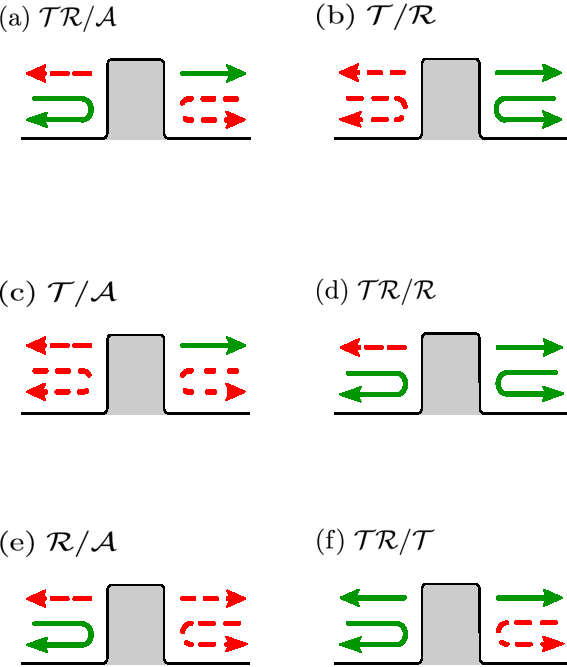
\includegraphics[width = 0.9\columnwidth]{Figures/PotentialCasesPT.pdf}
\caption{(Color online) Devices with asymmetric scattering (limited to scattering coefficients being 0 or 1).  The dashed and continuous lines represent respectively zero or one
for the moduli of the scattering amplitudes; the bended lines are for reflection amplitudes, and the straight lines for transmission:
(a) One-way mirror ($\cal{TR/A}$); (b) One-way barrier ($\cal{T/R}$); (c) One-Way T-filter ($\cal{T/A}$);
(d) Mirror \& 1-way transmitter ($\cal{TR/R}$); (e) One-way R-filter ($\cal{R/A}$); (f) Transparent, one-way
reflector ($\cal{TR/T}$).
The letter codes summarize the effect of left and right incidence, separated by a  slash ``$/$''.
${\cal T}$ or ${\cal R}$ on one side of the slash indicate a unit
transmission or reflection coefficient
for  incidence from that side, whereas the absence of one or the other letter corresponds to zero coefficients.
An ${\cal A}$ denotes ``full absorption'', i.e., both moduli of reflection and transmission amplitudes are zero for incidence from one side.
For example,  $\cal{TR/A}$ means unit modulus transmission
and reflection from the left and total absorption from the right.
\label{cases}}
\end{figure}

%The definition of generalized symmetries, and their physical implications when combined with generalized unitarity relations are analyzed in Section
%\ref{gs}.
%In Section \ref{examples}, we  design non-local potentials to implement the different asymmetric devices
%for a specific incident momentum.
%Sec. \ref{ext} provides an example of how to extend the domain of incident momenta
%for which the device works ideally.
%The final section summarizes the results and discusses open questions.

% ----------------------------------------------------------------------------------------------
\begin{landscape}
  \begin{table}
    \caption{Symmetries of the potential classified in terms of the commutativity or pseudo-hermiticity of $H$ with the elements of
    Klein's 4-group  $\{1,\Pi,\theta,\Pi\theta\}$ (second column). The first column sets a simplifying roman-number code for each symmetry.
    The relations among potential matrix elements are given in coordinate and momentum representations in the third and fourth columns.
    The fifth column gives the relations they imply in the matrix elements of $S$ and/or $\widehat{S}$ matrices ($S$ is for scattering by $H$
    and $\widehat{S}$ for scattering by $H^\dagger$). From them  the next four columns set the relations implied on scattering amplitudes.
    Together with generalized unitarity relations (\ref{gur}) they also imply relations for the moduli (tenth column), and phases (not shown). The last two columns indicate the possibility to achieve perfect asymmetric transmission or reflection:  ``${P}$" means possible (but not necessary),
    ``No'' means impossible.  In some cases ``$P$" is accompanied by a condition that must be satisfied.\vspace*{.2cm}
    \label{table2}}
    \centering
    \scalebox{0.75}{
    \begin{tabular}{cccccccccccc}
      %\hline
      Code & Symmetry&  $\langle x|V|y\rangle=$ & $\langle p|V|p'\rangle=$ & $\langle p|S|p'\rangle=$ & $T^l\!=$ & $T^r\!=$ & $R^l\!=$& $R^r\!=$& from eq. (\ref{gur})&$|T^l|\!=\!1$&$|R^l|\!=\!1$
      \\
      &&&&&&&&&&$|T^r|\!=\!0$&$|R^r|\!=\!0$
      \\
      \hline
      I & $1H=H1$ &   $\langle x|V|y\rangle$ & $\langle p|V|p'\rangle$ & $\langle p|S|p'\rangle$ & $T^l$ & $T^r$ & $R^l$ & $R^r$ & & $P$ & $P$
      \\
      II & $1H=H^\dagger 1$ &  $\langle y|V|x\rangle^*$ & $\langle p'|V|p\rangle^*$ &$\langle p|\widehat{S}|p'\rangle$ & $\widehat{T}^l$& $\widehat{T}^r$ & $\widehat{R}^l$ & $\widehat{R}^r$
      & $|T^l|\!=\!|T^r|$, $|R^l|\!=\!|R^r|$&No&No
      \\
      III & $\Pi H=H\Pi$ &  $\langle -x|V|-y\rangle$ & $\langle -p|V|-p'\rangle$ &$\langle -p|S|-p'\rangle$ & $T^r$ & $T^l$ & $R^r$ & $R^l$& $|T^l|\!=\!|T^r|$,$ |R^l|\!=\!|R^r|$ &No&No
      \\
      IV & $\Pi H=H^\dagger \Pi$ &  $\langle -y|V|-x\rangle^*$ & $\langle -p'|V|-p\rangle^*$ & $\langle -p|\widehat{S}|-p'\rangle$ & $\widehat{T}^r$ & $\widehat{T}^l$ & $\widehat{R}^r$ & $\widehat{R}^l$&&$P$, $R^rR^{l*}=1$&$P$, $T^r{T^l}^*=1$
      \\
      V & $\Theta H=H\Theta$ &  $\langle x|V|y\rangle^*$& $\langle -p|V|-p'\rangle^*$ & $\langle -p'|\widehat{S}|-p\rangle$ & $\widehat{T}^r$ & $\widehat{T}^l$ & $\widehat{R}^l$& $\widehat{R}^r$
      &$|R^l|=|R^r|$&$P$, $|R^{r,l}|=1$&No
      \\
      VI & $\Theta H=H^\dagger\Theta$ &  $\langle y|V|x\rangle$& $\langle -p'|V|-p\rangle$ & $\langle -p'|S|-p\rangle$ & $T^r$& $T^l$ & $R^l$& $R^r$&$|T^l| = |T^r|$&No&$P$
      \\
      VII & $\Theta\Pi H=H\Theta \Pi$ &  $\langle -x|V|-y\rangle^*$ & $\langle p|V|p'\rangle^*$ & $\langle p'|\widehat{S}|p\rangle$ &$\widehat{T}^l$& $\widehat{T}^r$ & $\widehat{R}^r$& $\widehat{R}^l$&$|T^l|=|T^r|$&No&$P$, $|T^{r,l}|=1$
      \\
      VIII& $\Theta\Pi H=H^\dagger \Theta \Pi$ &  $\langle -y|V|-x\rangle$ & $\langle p'|V|p\rangle$ & $\langle p'|S|p\rangle$ & $T^l$ & $T^r$ & $R^r$ & $R^l$&$|R^l|=|R^r|$&$P$&No
      %\\
      %\hline
    \end{tabular}}
  \end{table}
\end{landscape}

% ----------------------------------------------------------------------------------------------




\section{Generalized symmetries}


The detailed technical and formal background for the following can be found in
a previous review on 1D scattering by complex potentials \cite{Muga2004}, a companion to this article
for those readers willing to reproduce the calculations in detail.
The Supplemental Material (Sec. I)  provides also a minimal kit of scattering theory formulae that may be
read first to set basic concepts and notation.
The notation is essentially as in \cite{Muga2004}, but it proves convenient to use
for the potential matrix (or kernel function) in coordinate representation
two different forms, namely $\langle x|V|y\rangle=V(x,y)$. ``Local'' potentials are those
for which $V(x,y)=V(x)\delta(x-y)$.
%We will use the expression
%potential also for the potential matrix during this paper.



%
For hermitian  Hamiltonians, symmetries are represented by the commutation of
a symmetry operator with the Hamiltonian.
%For time-independent Hamiltonians
%the symmetry operator represents a conserved quantity.
% and, when
%applied to an eigenstate of $H$, it produces a degenerate eigenstate.
In scattering theory, symmetry plays an important role  as it implies relations among
the S-matrix elements beyond those implied by its unitarity, see e.g. \cite{Taylor1972} and, for scattering in one dimension,
Sec. 2.6 in \cite{Muga2004}.


Symmetries are also useful for  non-hermitian Hamiltonians, but the mathematical and conceptual
framework must be generalized. We consider that a unitary or antiunitary
%
%unitary or antiunitary symmetry transformation
operator $A$ represents a symmetry of $H$ if it satisfies
at least one of these relations,
%
\begin{eqnarray}
AH&=&HA,
\label{symm}
\\
AH&=&H^\dagger A.
\label{pseudo}
\end{eqnarray}
%
For a right eigenstate of $H$, $|\psi\rangle$,
with eigenvalue $E$, eq. (\ref{symm}) implies that
$A|\psi\rangle$ is also a right  eigenstate of $H$, with the
same eigenvalue if $A$ is unitary, and with the complex conjugate eigenvalue $E^*$ if $A$ is antiunitary.
Equation (\ref{pseudo}) implies that $A|\psi\rangle$ is a right eigenstate of $H^\dagger$
with eigenvalue $E$ for $A$ unitary or $E^*$ for $A$ antiunitary, or a left eigenstate of $H$ with eigenvalue $E^*$ for $A$ unitary, or $E$
for $A$ antiunitary. For real-energy scattering
eigenfunctions in the continuum, the ones we are interested in here, $E^*=E$.
When eq. (\ref{pseudo}) holds we say that $H$ is $A$-pseudohermitian \cite{Mostafazadeh2010}.
Parity-pseudohermiticity has played an important role as being equivalent to space-time reflection (PT) symmetry for {\it local} potentials
 \cite{Mostafazadeh2010,Znojil2015}. A large set of these equivalences
will be discussed below.
A relation of the form (\ref{pseudo}) has been also used with differential operators  to get real spectra beyond
PT-symmetry for local potentials  \cite{Nixon2016,Nixon2016a}.

Here we consider
%that $H$ may be non-local, and
$A$ to be a member of the
Klein 4-group $K_4=\{1,\Pi, \Theta, \Pi\Theta\}$ formed by unity, the parity operator $\Pi$, the antiunitary time-reversal operator $\Theta$, and their product
$\Pi\Theta$. This is a discrete, abelian group.
We also assume that the  Hamiltonian is  of the form $H=H_0+V$, with $H_0$, the kinetic energy operator of the particle,
being hermitian and
satisfying $[H_0,A]=0$ for all members of the group, whereas the potential $V$ may be non-local in position representation.
The  motivation to use Klein's group is that the eight relations implied by eqs. (\ref{symm}) and (\ref{pseudo}) generate all
possible symmetries of a non-local potential due to the identity, complex conjugation, transposition, and sign inversion,
both in coordinate or momentum representation, see table \ref{table2}, where each symmetry has been labeled by a roman number.
Interesting enough, in this classification hermiticity (symmetry II in  table \ref{table2})
may be regarded as $1$-pseudohermiticity.

\begin{table}
\caption{Equivalences among symmetries for the potential elements.
Given the symmetry of the upper row, the table provides the equivalent symmetries.
For example, if II is satisfied, then III=IV holds. In words, if the potential is hermitian,  parity symmetry amounts to
parity pseudohermiticity. In terms of the matrix elements of the potential, if  $\langle x|V|y\rangle=\langle y|V|x\rangle^*$ {\it and also}
$\langle x|V|y\rangle=\langle -x|V|-y\rangle$, $\forall (x,y)$, then $\langle x|V|y\rangle=\langle -y|V|-x\rangle^*$ holds as well. One may proceed similarly for all other relations.
The commutation with the identity (I) is excluded as this symmetry is satisfied by all potentials.\vspace*{.2cm}
 \label{tablee}}
\centering
\scalebox{0.9}{
\begin{tabular}{ccccccc}
%\hline
II & III& IV& V& VI & VII &VIII
\\
\hline
III=IV & II=IV & II=III & II=VI &II=V&II=VIII&II=VII
\\
V=VI&V=VII&V=VIII&III=VII&III=VIII&III=V&III=VI
\\
VII=VIII&VI=VIII&VI=VII&IV=VIII&IV=VII&IV=VI&IV=V
%\\
%\hline
\end{tabular}}

\end{table}

Examples on how to find the relations in the fifth column of table \ref{table2} of $S-$ and $\widehat{S}$-matrix elements (for scattering by $H$ and $H^\dagger$ respectively)
are provided in
ref. \cite{Muga2004}, where the symmetry types III, VI, and VII where worked out. Similar manipulations, making use of the action of unitary or antiunitary operators
of Klein's group on M\"oller operators, help to
complete the  table.
%$S$ or $\widehat{S}$ are not unitary in general for nonhermitian potentials
%but may be combined to set generalized unitarity relations, $\widehat{S}^\dagger S=S\widehat{S}^\dagger=1$.
%,
%see eq. (S8) for the explicit relations implied among the scattering amplitudes.

From the fifth column in table 1, equivalences among the amplitudes for left and right incidence
for scattering by $H$, ($T^{l,r}, R^{l,r}$) or $H^\dagger$  ($\widehat{T}^{l,r}, \widehat{R}^{l,r}$),
are deduced, see the Supplemental Material  and the four columns for
$T^{l,r}$, and $R^{l,r}$ in table \ref{table2}.
Together with the generalized unitarity relations $\widehat{S}^\dagger S=S\widehat{S}^\dagger=1$,
which in terms of amplitudes take the form \cite{Muga2004}
%(\ref{gur}),
%
\begin{eqnarray}
\widehat T^l T^{l*} + \widehat R^l R^{l*} = 1,
\nonumber\\
\widehat T^r T^{r*} + \widehat R^r R^{r*} = 1,
\nonumber\\
\hat T^{l*} R^r + T^r \widehat R^{l*} = 0,
\nonumber\\
T^l \widehat R^{r*} + \widehat T^{r*} R^l = 0,
\label{gur}
\end{eqnarray}
%
these equivalences  between the amplitudes
 imply further consequences on the amplitudes' moduli (tenth column of table \ref{table2}) and phases (not shown).
 The final two columns use the previous results to determine if perfect asymmetry is possible for transmission or reflection.
 This makes evident that hermiticity (II) and parity (III) preclude, independently, any asymmetry in the scattering coefficients;
 PT-symmetry (VII) or  $\Theta$-pseudohermiticity
 (VI) forbid transmission asymmetry (all local potentials  satisfy automatically
 symmetry VI),  whereas time-reversal symmetry (i.e., a real potential in coordinate space)
 (V) or  PT-pseudohermiticity (VIII) forbid reflection asymmetry.
 A caveat is that asymmetric effects forbidden by a certain symmetry in the linear (Schr\"odinger)
 regime considered in this paper might not be forbidden in a non-linear regime \cite{Xu2014}, which goes beyond our present scope.
 %
 %
 %\subsection{Double symmetries and equivalences among symmetries}
 %
 %



 The occurrence of one particular symmetry in the potential (conventionally  ``first symmetry'')
 does not exclude a second symmetry to be satisfied as well.
 When a double symmetry holds, excluding the identity,  the ``first'' symmetry  implies the equivalence of the second symmetry with a third symmetry.
 We have already mentioned that $\Pi$-pseudohermiticity (IV) is equivalent to $PT$-symmetry (VII) for local potentials.
 Being local is just one particular way to satisfy symmetry VI, namely $\Theta$-pseudohermiticity. The reader may verify with the aid of
 the third column for $\langle x|V|y\rangle$  in table \ref{table2}, that indeed, if symmetry VI is satisfied (first symmetry), symmetry IV has the same effect as symmetry VII.
 They become equivalent. Other well known example is  that for a local potential (symmetry VI is satisfied), a real potential in coordinate space  is necessarily hermitian,
 so symmetries V and II become equivalent.
 These examples are just particular cases of the full set of equivalences given in table \ref{tablee}.
%This Table can be written down using the coordinate representation of the potential for the different symmetries,
%or also acting on any symmetry relation in Eqs. (\ref{symm}),(\ref{pseudo}) with the other members of $K_4$, assuming a second symmetry
%to hold, and using the product table of
% Klein's group.
%
%
%
%
%\subsection{Asymmetric devices}
%
%
%
%
%%%%%%%%%
\begin{landscape}
  \begin{table}
    \caption{Device types for  transmission and/or reflection asymmetry, restricted to 1 or 0 moduli for the scattering amplitudes.
    % (i.e., zero scattering amplitudes for transmission and reflection from the right).
    The fifth column indicates the symmetries in table \ref{table2} that forbid the device. Figures S2, S3, S5 and S6 can be found in the supplemental material to this paper.\vspace*{.2cm}}
    \label{table1}
    \centering
    \scalebox{0.85}{
    \begin{tabular}{ccccccc}
      %\hline
      Device type & Left incidence& Right incidence&Code& Forbidden by & Example
      \\
      \hline
      One-way mirror&transmits and reflects&absorbs&$\cal{TR/A}$&II, III, IV, V, VI,  VII, VIII& fig. S1
      \\
      One-way barrier&transmits&reflects&$\cal{T/R}$&II, III, IV, V, VI, VII, VIII&fig. S2
      \\
      One-way T-filter&transmits&absorbs&$\cal{T/A}$&II, III, IV, V, VI, VII&fig. \ref{fig_device_T_A}, S3
      \\
      Mirror\&1-way transmitter&transmits and reflects&reflects&$\cal{TR/R}$&II, III, VI, VII&fig. S4
      \\
      One-way R-filter&reflects&absorbs&$\cal{R/A}$&II, III, IV, V, VII, VIII&\cite{Huang2016}
      \\
      Transparent 1-way reflector&transmits and reflects&transmits&$\cal{TR/T}$& II, III, V, VIII
      & figs. \ref{fig_reflector}, S5
      %\\
      %\hline
    \end{tabular}}
  \end{table}
\end{landscape}


\begin{table}
\caption{Device types allowed for a given symmetry.
\vspace*{.3cm}\label{tableComp}}
\centering
\scalebox{0.9}{
\begin{tabular}{cc}
%\hline
Symmetry& Allowed devices
\\
\hline
I&All types
\\
II&None
\\
III&None
\\
IV&$\cal{TR/R,TR/T}$
\\
V&$\cal{TR/R}$
\\
VI & $\cal{R/A, TR/T}$
\\
VII&$\cal{TR/T}$
\\
VIII&$\cal{T/A,TR/R}$
%\\
%\hline
\end{tabular}}

\end{table}





Combining the information of the last two-columns in table \ref{table2} with the additional condition that all scattering coefficients
be 0 or 1 we elaborate table \ref{table1}, which provides
%names for the six possible types of devices, a convenient letter code
%that summarizes the effect of left/right incidence, and
the symmetries
that do not allow the implementation of the devices in fig. \ref{cases}.
%The six types of devices are also summarized schematically in Fig. \ref{cases}.
The complementary table \ref{tableComp} gives instead the symmetries that allow, but do not necessarily imply,
a given device type.
The device denominations in fig. \ref{cases} or table \ref{table1} are intended as short and meaningful, and do not necessarily coincide with
some extended terminology, in part because the range of possibilities is broader here than those customarily considered, and because we
use a 1 or 0 condition for the moduli.
For example, a device with reflection asymmetry and with $T^r=T^l=1$ would in our case be a particular
``transparent, one-way reflector'', as full transmission occurs from both sides.
This effect has however become popularized as ``unidirectional invisibility'' \cite{Lin2011,Yin2013}.
A debate on terminology is not our main concern here, and the use of a code system
as the one proposed will be instrumental in avoiding misunderstandings.

%%%%%%%%%

\begin{figure}
\begin{center}
(a)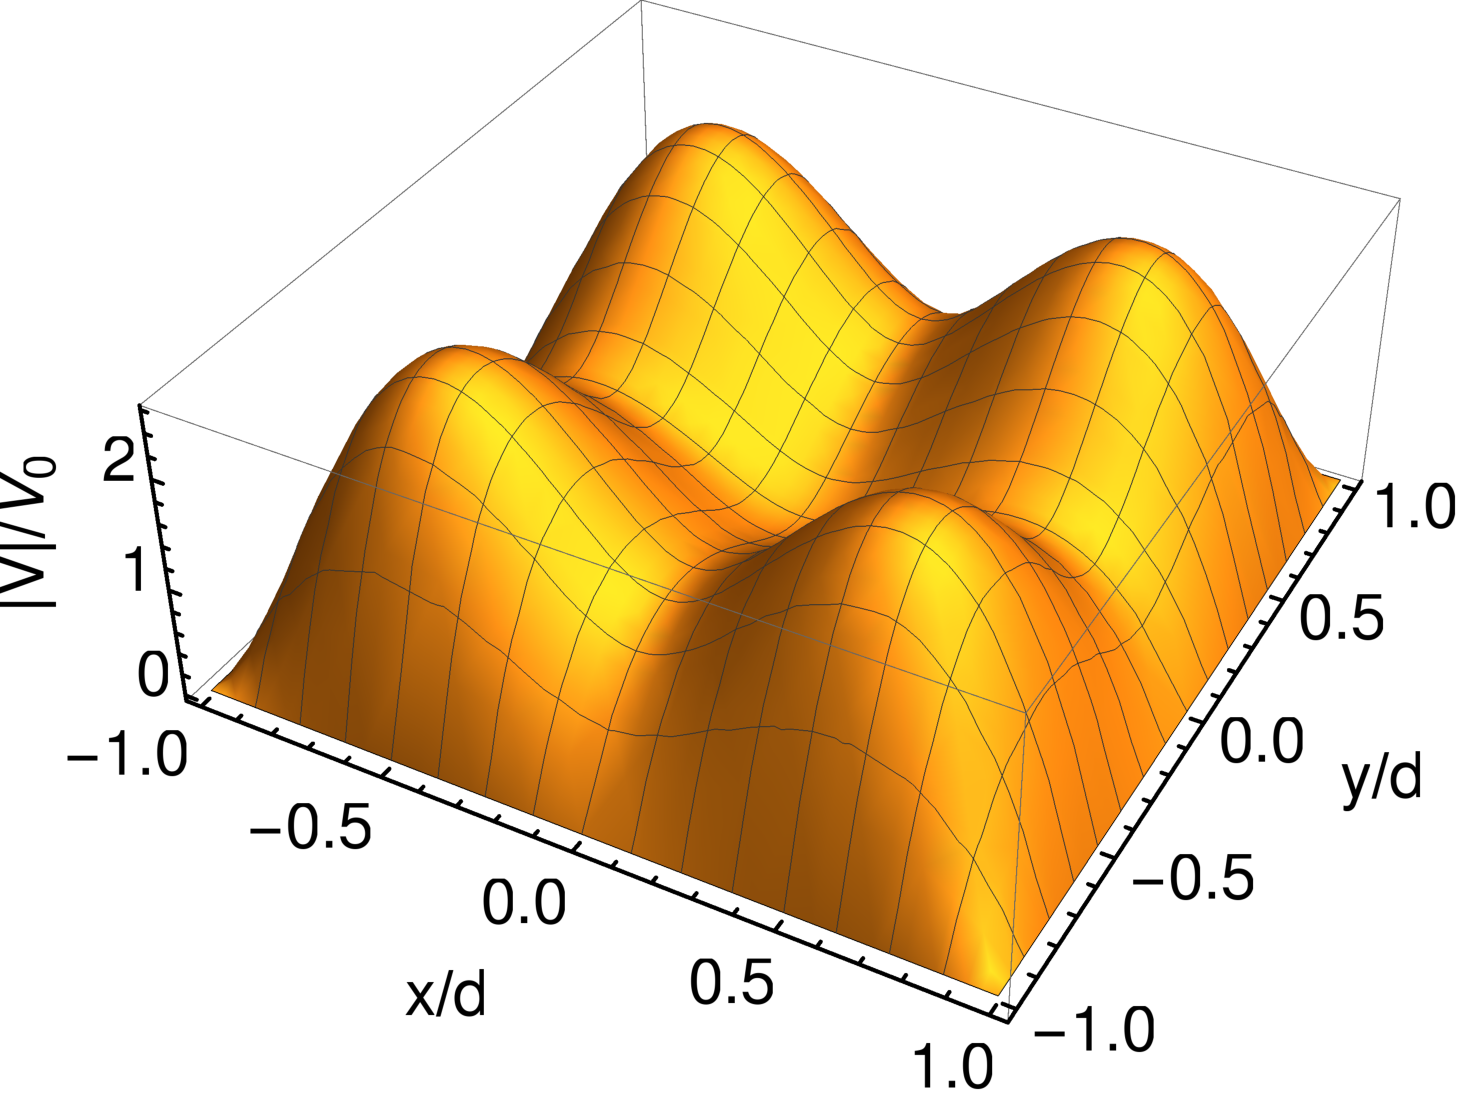
\includegraphics[width = 0.6\columnwidth]{Figures/fig_T_A_pot_abs.pdf}\\
(b)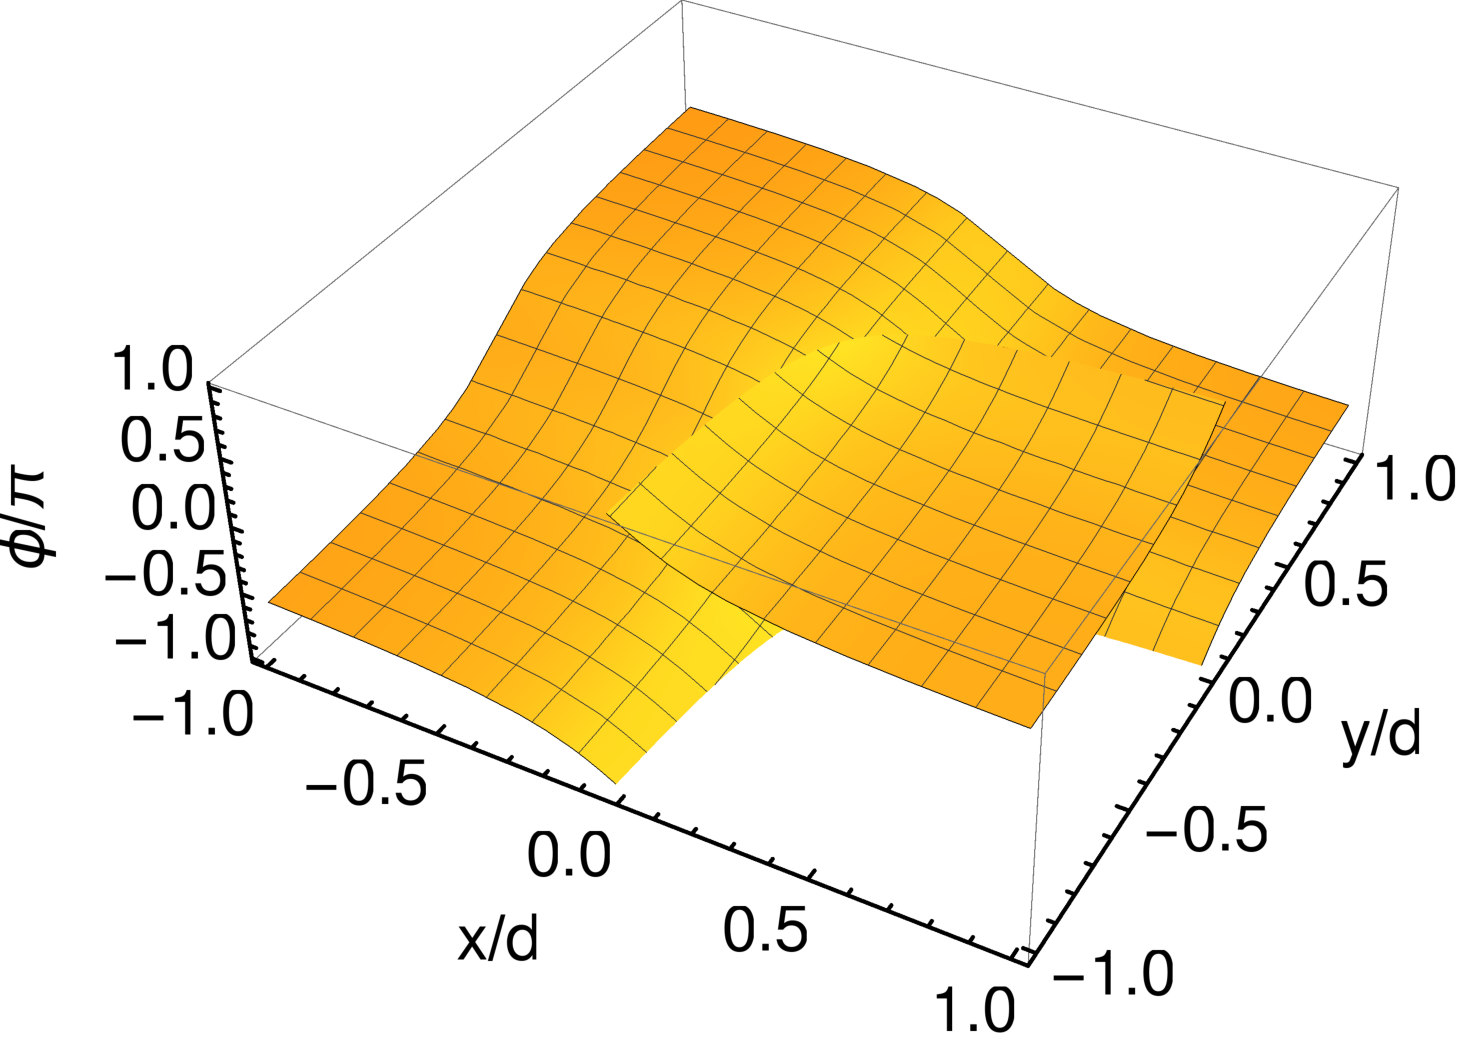
\includegraphics[width = 0.6\columnwidth]{Figures/fig_T_A_pot_arg.pdf}\\
(c)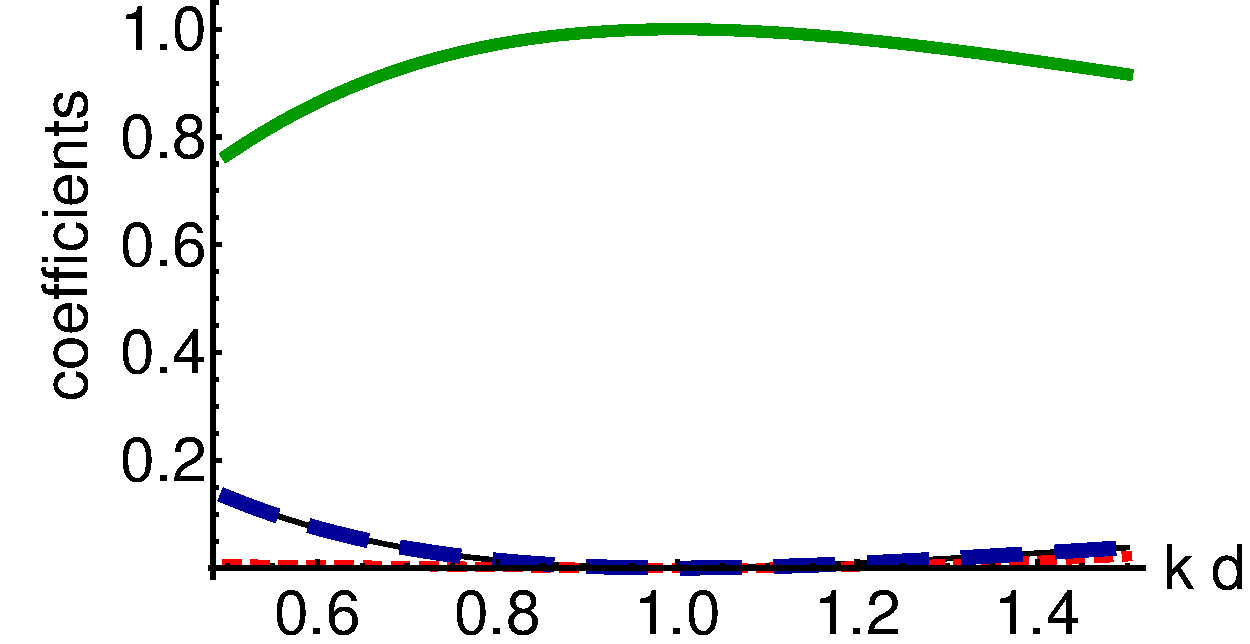
\includegraphics[width = 0.6\columnwidth]{Figures/fig_T_A_prob.pdf}
\end{center}
\caption{(Color online) One-way T-filter ($\cal{T/A}$, $\left|T^l\right|=1,T^r=R^l=R^r=0$) with  potential $V(x,y)=|V(x,y)|e^{i\phi(x,y)}$ set
for $k_0 = 1/d$.
(a) Absolute value $\left| V(x,y) \right|$;    (b) Argument $\phi(x,y)$;
(c) Transmission and reflection coefficients:
$\left| R^l \right|^2$ (black, solid line), $\left| T^l \right|^2$ (green, solid line),
$\left| R^r \right|^2$ (blue, tick, dashed line), $\left| T^r \right|^2$ (red, dotted line). $V_0 = \hbar^2/(2m d^3)$.\label{fig_device_T_A}}
\end{figure}


%
%
%

\section{Designing potentials for asymmetric devices\label{examples}}

\begin{figure}
\begin{center}
(a) 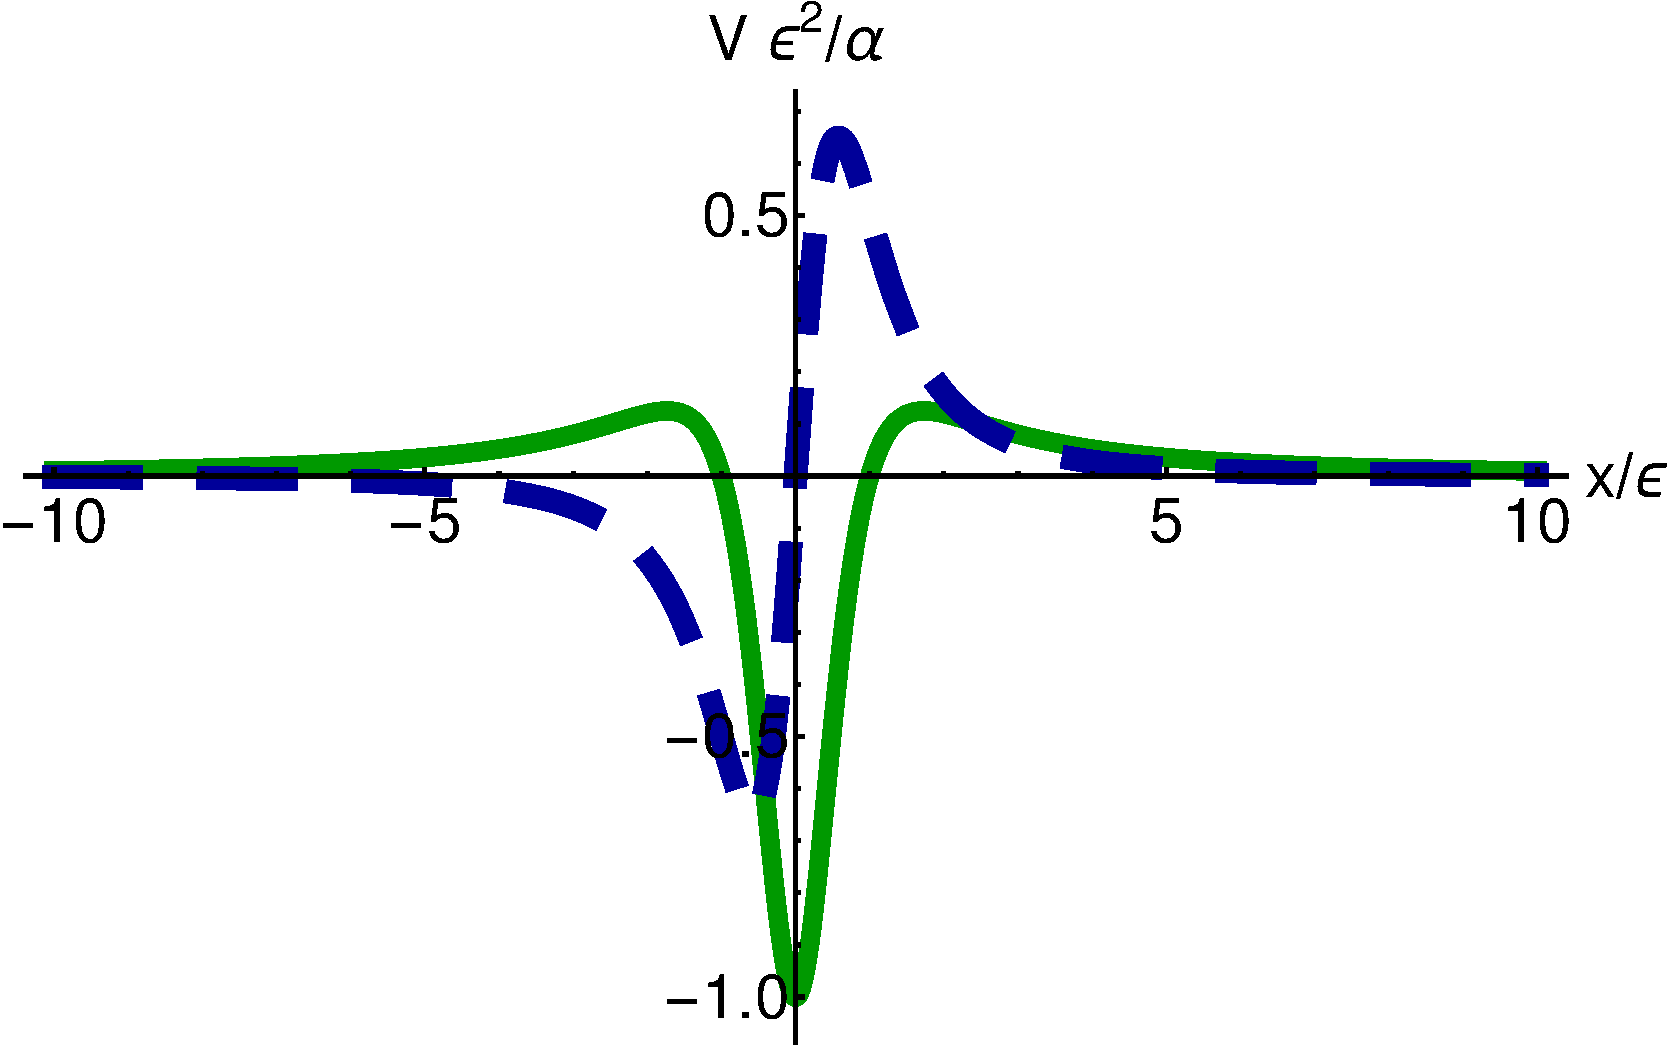
\includegraphics[width = 0.6\columnwidth]{Figures/fig_TR_T_local_pot.pdf}\\
(b) 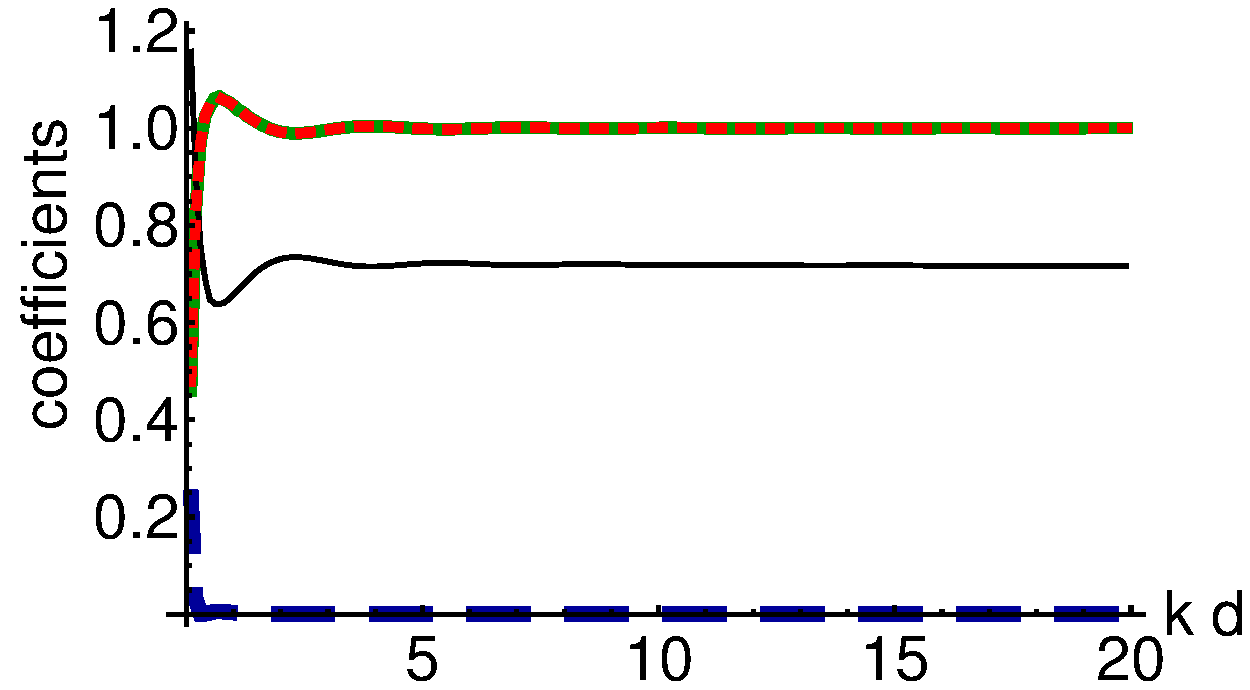
\includegraphics[width = 0.6\columnwidth]{Figures/fig_TR_T_local_prob_1.pdf}\\
(c) 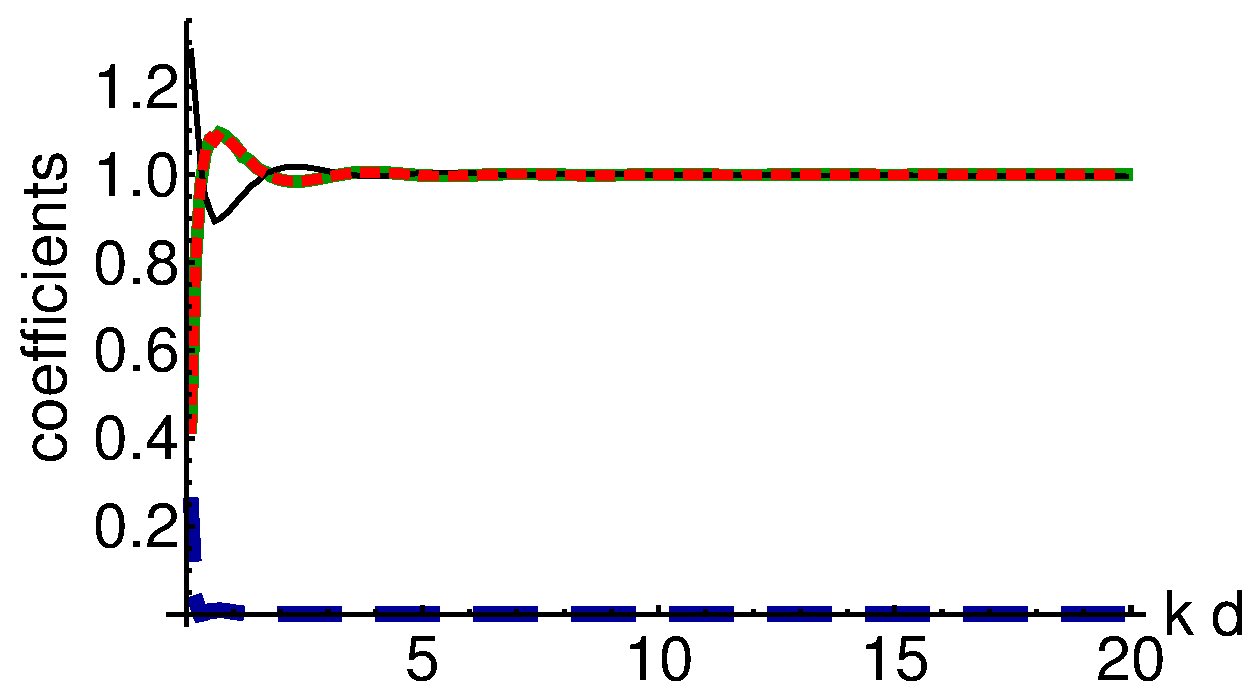
\includegraphics[width = 0.6\columnwidth]{Figures/fig_TR_T_local_prob_2.pdf}
\end{center}
\caption{\label{fig_reflector}(Color online) Transparent 1-way reflector with a local PT potential:
(a) Approximation of the potential (\ref{num}), real part (green solid line), imaginary part (blue dashed line).
(b,c) Transmission and reflection coefficients versus momentum $k d$;
left incidence: $\left| R^l \right|^2$ (black, solid line), $\left| T^l \right|^2$ (green, solid line);
right incidence: $\left| R^r \right|^2$ (blue, tick, dashed line), $\left| T^r \right|^2$ (red, dotted line, coincides with green, solid line).
$\epsilon/d = 10^{-4}$.
(b) $\alpha= 1.0 \hbar^2/(4\pi m)$ (c) $\alpha = 1.225 \hbar^2/(4\pi m)$
(the black, solid line coincides here mostly with the red, dotted and green, solid lines).
\label{fig_TR_T_local}}
\end{figure}


We will show  how to design non-local potentials
leading to the asymmetric devices.
For simplicity we look for  non-local potentials $V(x,y)$ with local support
that vanish  for $|x| >d$ and $|y| >d$.

Inverse scattering proceeds similarly to \cite{Palao1998},
by imposing an ansatz
for the wavefunctions and the potential
in the stationary Schr\"odinger equation
%
\begin{eqnarray}
\frac{\hbar^2k^2}{2m} \psi (x) = - \frac{\hbar^2}{2m} \frac{d^2}{dx^2} \psi (x)
+\!\!\int_{-d}^d \!dy V(x, y) \psi(y).
\label{Schroedinger}
\end{eqnarray}
%
The free parameters are fixed making use of the boundary conditions.
The form of the wavefunction incident from the left is
$\psi_l(x) = e^{i k x} + R^l e^{-i k x}$ for $x < -d$ and $\psi_l (x) = T^l e^{i k x}$ for $x > d$,
where  $k=p/\hbar$.
The wavefunction incident from the right is instead
$\psi_r(x) = e^{-ikx} T^r$ for $x < -d$ and $\psi_r (x) = e^{-i k x} + R^r e^{i k x}$ for $x > d$.

Our strategy is to assume  polynomial forms for the two wavefunctions in the interval $|x| < d$,
$\psi_l (x) = \sum_{j=0}^5 c_{l,j} x^j$ and $\psi_r (x) = \sum_{j=0}^5 c_{r,j} x^j$, and also a
polynomial ansatz of finite degree for the potential $V(x,y) = \sum_i \sum_j v_{ij} x^i y^j$.
Inserting these ansatzes in eq. (\ref{Schroedinger}) and from the conditions that $\psi_{l,r}$
and their derivatives must be continuous, all coefficients $c_{l,j}\,,c_{r,j}$ and $v_{ij}$ can be determined.
Symmetry properties of the potential can also be imposed via additional conditions on
the potential coefficients $v_{ij}$. For example we may use this method to obtain a one-way T-filter ($\cal{T/A}$) device (third device in table \ref{table1}) with a nonlocal PT-pseudohermitian potential (symmetry VIII of table \ref{table2}) for a chosen wavevector $k = k_0$. The absolute value and argument of the resulting potential $V(x,y)$ are shown in figs. \ref{fig_device_T_A}(a) and \ref{fig_device_T_A}(b) together with its scattering coefficients as function of the incident wave vector, fig. \ref{fig_device_T_A}(c). As can be seen in fig. \ref{fig_device_T_A}(c) the imposed scattering coefficients are fulfilled exactly for the chosen wavevector. They are also satisfied approximately in a neighborhood of $k_0$. In the  Supplemental Material, Sec. II, we give further details about the construction of this potential and we work out other asymmetric devices of fig. \ref{cases}.
%
% ---------------------------------------- Asymmetric Reflection -----------------------------------
%
%
%
%

%
%%%%%%%%%%%%%%%%%%%%%%%%%%%%%%%%%%%%%%%%%%%%%%

%%%%%%%%%%%%%%%%%%%%%%%%%%%%%%%%%%%%%%%%%%%%%
%

\section{Extending the scattering asymmetry to a broad incident-momentum domain\label{ext}}
%
%
%
%
The inversion technique just described may be generalized
to extend the range of incident momenta for which the potential works by imposing additional
conditions and increasing correspondingly the number of parameters in the wavefunction ansatz,
for example we may impose that the derivatives of the  amplitudes,  in one or more orders,  vanish at $k_0$,
or  0/1 values for the coefficients not only at  $k_0$ but at a series of grid points $k_1$, $k_2$, ... $k_N$,
as in \cite{Brouard1994,Palao1998a,Palao1998,Muga2004}.

Here we put forward instead a method that provides a very broad working-window domain.
While we make formally use of the Born approximation, the exact numerical
computations demonstrate the robustness and accuracy of the approach to achieve that objective by
making use of an adjustable parameter in the potential. The very special role of the Born approximation in inverse problems has been
discussed and demonstrated in \cite{Snieder1990,Mostafazadeh2014,Horsley2015}.
Specifically we study a transparent one-way reflector ${\cal{TR/T}}$.
Our aim is now to find a local PT-symmetric potential such that asymmetric reflection results,
$T^l = T^r = 1, R^r = 0, |R^l|=1$ for a broad range of incident momenta. A similar goal
was pursued in \cite{Longhi2014} making use of a supersymmetric transformation,
without imposing $|R^l|=1$.

In the Born approximation and for a local potential $V(x)$, the reflection amplitudes take the simple form
%
\begin{eqnarray}
R^l=-\frac{2\pi i m}{p}\langle -p|V|p\rangle,
\;
R^r=-\frac{2\pi i m}{p}\langle p|V|-p\rangle.
\end{eqnarray}
%
Defining the Fourier transform
%
\begin{eqnarray}
\widetilde V (k) = \frac{1}{\sqrt{2\pi}} \int_{-\infty}^\infty dx \, V(x) e^{-i k x}
\end{eqnarray}
%
we get for $k=p/\hbar>0$:
%
\begin{eqnarray}
R^l=-\frac{\sqrt{2\pi} i m}{k \hbar^2} \widetilde V (-2k),
\;
R^r=-\frac{\sqrt{2\pi} i m}{k\hbar^2} \widetilde V (2 k).
\end{eqnarray}
%
Assuming that the potential is local and PT-symmetrical, we calculate the transition coefficient
from them using generalized unitarity as
$|T|^2=1-{R^r}^*R^l$.

To build a ${\cal{TR/T}}$ device we demand:
$\widetilde V(k) = \sqrt{2\pi} \alpha k$ ($k < 0$) and $\widetilde V(k) = 0$ ($k \ge 0$).
By inverse Fourier transformation, this implies
%
\begin{eqnarray}
V(x) &=&
%-\alpha \frac{\partial}{\partial x} \left[P \frac{1}{x} + i \pi \delta(x) \right]
%\nonumber\\
%&=&
-\alpha \frac{\partial}{\partial x} \lim_{\epsilon\to 0} \frac{1}{x - i \epsilon}
= \alpha \lim_{\epsilon\to 0} \frac{1}{(x - i \epsilon)^2}
\nonumber\\
%&=& \alpha \lim_{\epsilon\to 0} \frac{(x + i \epsilon)^2}{(x^2 + \epsilon^2)^2}\\
&=& \alpha \lim_{\epsilon\to 0} \left[\frac{x^2 - \epsilon^2}{(x^2 + \epsilon^2)^2} + i
\frac{2 x\epsilon}{(x^2 + \epsilon^2)^2}\right],
\label{num}
\end{eqnarray}
%
which is indeed a local, $PT$-symmetric potential for $\alpha$ real.
$\alpha$ is directly related to the reflection coefficient, within the Born approximation,
$R^l = 4 \pi i m \alpha/\hbar^2$. As the Born approximation may differ from exact results
we shall keep $\alpha$ as an adjustable parameter
in the following.

In a possible physical implementation, the potential in eq. (\ref{num}) will
be approximated by keeping a small finite $\epsilon>0$, see fig. \ref{fig_TR_T_local}(a).
%\begin{eqnarray}
%V(x) = \alpha \left[\frac{x^2 - \epsilon^2}{(x^2 + \epsilon^2)^2} + i
%\frac{2 x\epsilon}{(x^2 + \epsilon^2)^2}\right],
%\end{eqnarray}
%with a finite, small $\epsilon>0$.
Then, its Fourier transform is
$\widetilde V(k) = \sqrt{2\pi} \alpha k e^{\epsilon k}$ ($k < 0$) and $\widetilde V(k)=0$ ($k \ge 0$).
In figs. \ref{fig_TR_T_local}(b) and (c), the resulting coefficients for $\epsilon/d=10^{-4}$ and  two different values
of $\alpha$ are shown.  These figures have been calculated by
numerically solving the Schr\"odinger equation exactly.
% and demonstrate that
%$\alpha$ can indeed  be adjusted so that $\left| R^l \right|^2 \approx 1$.
Remarkably, the Born approximation contains all the information required to build the required potential shape
up to a global factor.  Such a prominent role of the Born approximation in inverse problems has been noted
in different applications \cite{Snieder1990,Mostafazadeh2014,Horsley2015}. For a range of $\alpha$, the potential gives $|R^r|\approx 0$, a nearly constant $|R^l|^2$, and
$|T^r|= |T^l|\approx1$  in a broad $k$-domain, see fig. \ref{fig_TR_T_local}(b). Adjusting  the value of $\alpha$, fig. \ref{fig_TR_T_local}(c),
sets $|R^l|\approx 1$ as desired.
%
%Remarkably, except for very low $k$,
%the potential is reflectionless from the right
%and provides full transmission independently of $\alpha$. As well, $|R^2|^2$ stays constant with respect to $k$ for different $\alpha$,
%so that that up to the adjustable parameter the Born approximation provides in fact the required potential shape, a surprising
%in inverse problems \cite{Snieder1990,Mostafazadeh2014,Horsley2015}.
%Figure \ref{fig_TR_T_local}(c) demonstrates that $\alpha$ can indeed be adjusted so that the  potential works
%as intended, i.e., as a transparent one-way reflector,  for a very broad range of $k$ values.

%
%
%
%
%
\section{Discussion}
%
%
Scattering asymmetries are necessary to develop technologically relevant devices such
as one-way mirrors, filters and  barriers, invisibility cloaks, diodes, or Maxwell demons.
So far much effort has been devoted to build and apply local  PT-symmetric potentials but the possible scattering asymmetries with them are
quite limited.
%This paper shows that to realize all possible devices it is necessary to go beyond local PT-potentials to
%ealize different asymmetric devices.
We find that six  device types with asymmetric scattering are possible
when imposing $0$ or $1$ scattering coefficients.
PT-symmetry can only realize one of them, but this symmetry  is just one among eight possible symmetries of complex non-local potentials.
The eight symmetries arise from the discovery that Klein's four-group
$\{1, \Pi, \Theta, \Theta\Pi\}$, combined with two possible relations among the Hamiltonian, its adjoint,
and the symmetry operators of the group, eqs. (1) and (2),
produce all possible  equalities among potential matrix elements after complex conjugation, coordinate inversion, the identity, and transposition.
In other words, to have all possible such equalities, the conventional definition of a symmetry $A$ in terms of its commutation with the Hamiltonian $H$ is not enough, and $A$-pseudohermiticity must be considered as well on the same footing.
Extending the concept of what a �symmetry� is for complex, non-local potentials is
a fundamental, far-reaching step of this work.
This group theoretical analysis and classification is not only esthetically pleasing, but also of practical importance, as it reveals
the underlying structure and span of the possibilities available in principle to manipulate the asymmetrical response of a potential
for a structureless particle.

%This paper brings to the fore the essential role of eight generalized symmetries to determine the
%transmission and reflection asymmetries by complex, and possibly nonlocal potentials.
%These symmetries are classified with the aid of the relations between
%unitary or antiunitary operators $1, \Pi, \Theta, \Theta\Pi$, which form Klein's 4-group,
%and $H$ or its adjoint.
%generically $A$, forming Klein's 4-group
%and correspond to $A$ either commuting with
%the Hamiltonian $H$, or intertwining
%$H$ and $H^\dagger$ as $AH=H^\dagger A$.
%The symmetries set equalities among the scattering
%amplitudes which, complemented by generalized unitarity relations, tell us which symmetries allow or disallow
%a certain device with asymmetric scattering. Simplifying the analysis by imposing $0$ or $1$ scattering coefficients,
%six possible device types exist.
%We provide examples of potentials
We provide potentials for the different asymmetric  devices including an example that works
in a broad domain of incident momenta.
%
Although the present theory is for the scattering of quantum particles, the analogies between quantum physics and optics suggest to extend the concepts and results for optical asymmetric devices.

Interesting questions left for future work are  the inclusion of other mechanisms for transmission and reflection asymmetries (for example
nonlinearities \cite{Xu2014,Konotop2016}, and  time dependent potentials \cite{Yu2009,Longhi2017}),
or a full discussion of the phases of the scattering amplitudes
in addition to the moduli emphasized here. In this paper the properties of the scattering amplitudes have been worked out assuming that the operator $A$ in the symmetry relations in eqs. (\ref{symm}) and (\ref{pseudo}) is a unitary/antiunitary operator in Klein's group.
We may generalize the study to include more general operators, possibly including differential operators, as was done in \cite{Konotop2017} for phase transitions of optical potentials, or the operator that swaps internal states or waveguides \cite{Kartashov2014,Zezyulin2017}.

We shall also examine in a complementary paper the physical realization of complex nonlocal effective potentials.
In a quantum optics scenario, simple examples were provided in \cite{Ruschhaupt2004a} based on applying the partitioning technique \cite{Feshbach1958,Feshbach1962}
to the scattering of a particle with internal structure. The experimental realization
of all new symmetries and devices may be challenging, e.g. to engineer the nonlocality in optics,
but there is much to gain.  We may expect progress similar to
the successful evolution from theory to actual devices in the sequence from the first mathematical
models of PT-symmetric potentials \cite{Bender1998}, to the proposal of an optical realization \cite{Ruschhaupt2005}, and to the actual experiments \cite{Guo2009},  even if considerable time lapses were needed between the three steps.
%
 %Asymmetric Scattering nonhermitian

%!TEX root = ../Thesis.tex
%Chapter 1

\chapter{Local rectification of heat flux}
\label{ChapterLocalRectification}
\lhead{Chapter X \emph{Local rectification of heat flux}} % Write in your own chapter title to set the page header
%
We present a chain-of-atoms model where heat is rectified, with different fluxes from the hot to the cold baths
located at the chain boundaries when the temperature bias is reversed. The chain is homogeneous except for boundary effects
and a local modification of the interactions
at one site, the ``impurity''. The rectification mechanism is due here to the localized impurity, the only asymmetrical element of the structure, apart from the externally imposed temperature bias,  and does not rely on putting in contact different materials or other known mechanisms such as grading or long-range interactions.  The effect survives if all interaction forces are linear except the ones for the impurity.
%
\newpage
%

\section{Introduction}

In spite of much work on thermal rectification
after the first model proposal in 2002 \cite{Terraneo2002} (for a broad perspective on heat rectification
see \cite{Roberts2011,Li2012}), the manipulation of phononic
heat fluxes is still far from being completely controlled as no efficient and feasible thermal diodes have been found \cite{Chen2015,Pereira2017}.
The thermal rectifier, a device where the heat
current changes when the temperature bias of the thermal baths at the boundaries is reversed,
is one of the key tools needed to manipulate heat currents and build thermal circuits.
A wealth of research is underway to meet the challenge posed by  a ``near standstill'' of the field \cite{Chen2015,Pereira2017},
combined with the prospects of widespread and impactful practical applications.
Together with experimental progress, at this stage work exploring new models is important to test possibilities that may become feasible as control capabilities improve \cite{Roberts2011}.
In this paper we propose,
motivated by previous work on ``atom diodes"  \cite{Ruschhaupt2004,Raizen2005}, a rectifying scheme
based on the effect of a local defect, or impurity,
in an otherwise homogeneous system.

To date, there have been several proposals of systems that could be used to rectify heat flows at the nanoscale.
A common scheme is based on coupling two or more different homogeneous segments, modelled with
chains of atoms with nonlinear interactions (which in this context means non-linear forces, i.e., anharmonic potentials) \cite{Terraneo2002,Li2004,Hu2006,Peyrard2006,Benenti2016}
or with a temperature and position dependent
conductivity assuming expressions for the heat current \cite{Peyrard2006,Hu2006a}.
%Other proposals \cite{Hu2006} make use of a two-segment Frenkel Kontorova model \cite {Li2004} finding size effects such us the reversal of the rectification as the size of the system increases, depending on the strength of the coupling between both segments.
Basic ingredients for thermal rectification have been considered to be  the asymmetry in the system and non-linear interactions
\cite{Zeng2008,Li2012,Benenti2016}, which lead to a temperature dependence of the phonon bands, or power spectral densities,  of the
weakly coupled \cite{Hu2006} segments. These bands match or mismatch at the interfaces, depending of the sign of the temperature bias, leading, respectively, to heat flow or insulating conditions. In fact, alternative mechanisms due to band mixing appear for stronger coupling
or long chains \cite{Hu2006}, and Pereira \cite{Pereira2017},  based on minimalist models,
has recently reformulated the conditions leading to rectification  as the combination of asymmetry plus the existence of some feature of the system that depends on the temperature (nonlinearity is certainly a possible cause of such dependence).
Other systems proposed are graded materials, such as a chain with an uneven distribution of mass \cite{Chang2006,Zeng2008,Chen2015}, and long-range interactions  have been shown to be able to amplify the rectification and avoid or mitigate the decay of the effect with system size \cite{Pereira2013,Chen2015}.
%Mass graded materials can be built, but up to now the rectification experimentally observed is small \cite{Chang2006}.
Also, recent models and experiments use asymmetrical homogeneous or inhomogeneous nanostructures and, in particular, graphene  \cite{Wang2014,Wang2017}.
Finally, we mention for completeness theoretical works
%farther from our model
that consider the use of a quantum system \cite{Roberts2011}, such as a three-level system, with each level coupled to a thermal bath \cite{Joulain2016}, or a double well with different frequencies to implement the asymmetry \cite{Katz2016}.

The model proposed in this paper is a one-dimensional chain of atoms where all, except one of them, are trapped in on-site harmonic potentials and interact with their nearest neighbours by Morse potentials (or also by harmonic
potentials in a simplified version). Unlike most chain models, the structural asymmetry is, except for the boundaries,
only in the impurity, which is subjected to a different on-site potential and interaction with one of its neighbors. The chain is connected to thermal baths at different temperatures at the boundaries.
Let us clarify our terminology:
The structural asymmetry we have in mind amounts,
to different interaction potentials of one or several atoms in the
chain (other than the boundary atoms) with neighbors on the right and on the left, and/or asymmetric onsite potentials. In this regard  chains with Morse interatomic potentials per se are not considered structurally asymmetric here as long as their parameters are the same on both sides of a given atom, even if a single Morse potential is obviously asymmetric with respect to its minimum \cite{Wang2015}.
%each end, and we have chosen the well known Nos\'e-Hoover model to simulate the thermal baths \cite{Martyna1992}.
%The manipulation of the potentials that affect one of the atoms makes the excitations easier to be transferred from one side, providing a mechanism for the inhomogeneity needed.

First, we shall describe the
%initial system used, that consists of a
homogeneous 1D chain, without the impurity,  %For this system, we numerically solve the dynamical equations, to show that the usual heat conduction applies. Once the system is connected to the baths at different temperature, after a transient time, the steady regime with constant value of the heat flux, $J$, is reached, and
and show its heat conduction behavior.
%Our goal is to obtain a system that presents a direction dependent heat flux when the positions of the baths are interchanged. With this aim,
Then  we modify the potentials for one of the atoms and demonstrate the rectification effect.


\section{Homogeneous one-dimensional chain}

We start with a homogeneous $1D$ chain with $N$ atoms coupled at both extremes to heat baths, at different temperatures $T_h$ and $T_c$ for ``hot" and ``cold" respectively. The baths are modeled with a Nos\' e-Hoover method as described in \cite{Martyna1992}.
Atoms $1$ and $N$ represent the first and the $N$-th atom in the chain, from left to right,
that will be in contact with the baths. All the atoms are subjected to on-site potentials and to nearest-neighbor interactions, and their equilibrium positions $y_{i0}$ are assumed to be equally spaced by a distance $a$.
$x_i= y_i-y_{i0}$,
$i=1,...,N$, represent the displacements from the equilibrium positions of the corresponding atoms
with positions $y_i$.

The classical Hamiltonian of the atom chain can be written in a general form as
%
\begin{equation}
\label{GH}
%GH=general Hamiltonian
H=\sum_{i=1}^{N} H_i,
\end{equation}
%
with
%
\begin{eqnarray}
\label{GH2}
%GH=general Hamiltonian
H_1&=&{{p^2_1} \over {2m}} +U_1(x_1)+V_L,
\nonumber\\
H_i&=&{{p^2_i} \over {2m}} +U_i(x_i)+V_i(x_{i-1},x_i)  \quad i=2,...,N-1,
 \nonumber\\
H_N&=&{{p^2_N} \over {2m}} +U_N(x_N)+V_N(x_{N-1},x_N) + V_R,
\end{eqnarray}
%
where the $p_i$ are the momenta, $U_i(x_i)$ is the on-site potential for the $i$th atom, and $V_i(x_{i-1},x_i)$ represents the atom-atom interaction potential. $V_R$ and $V_L$ are the interactions coupling the boundary atoms to the Nos\'e-Hoover thermostats, see \cite{Martyna1992}.

There are a large number of $1D$ models that obey this general Hamiltonian. Using different potentials for the trapping and interactions we would get different conductivity behaviors.
%%%%%%%%%%%%%%%%%%%%%%%
\begin{figure}
\centering
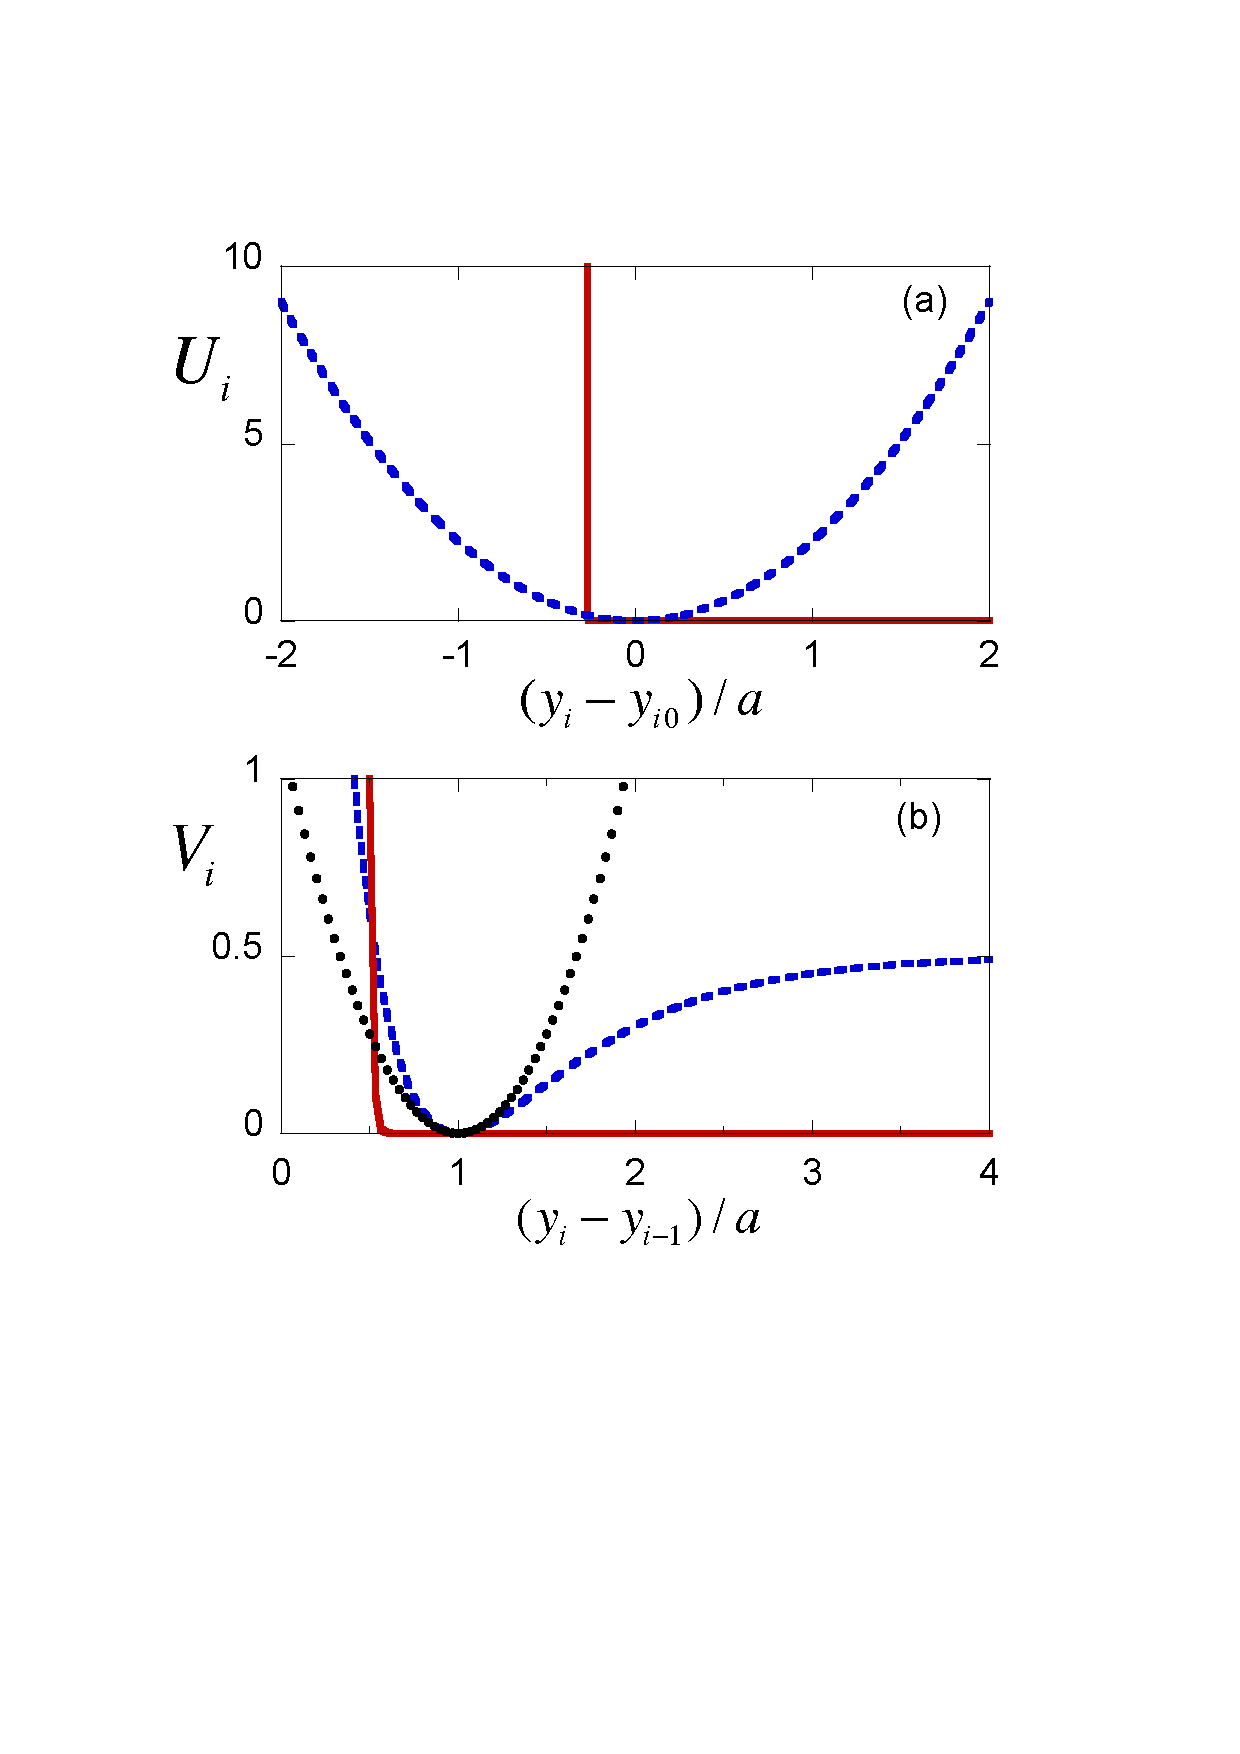
\includegraphics[width=8.8cm]{Figures/FIG1.pdf}
\caption{(Color online) (a) On-site potentials: harmonic potential centered at the equilibrium position of each atom (dashed blue line) as a function of the displacement from this position $x_i=y_i-y_{i0}$ in $a-$units, and the on-site potential for the impurity, $i=N/2+1$
($N$ even, red solid line). (b) Interaction potentials as a function of the distance between nearest neighbors: Morse potential
(blue dashed line) valid for all atoms except for $i=N/2+1$, $N$ even, where the modified potential (red solid line) is used.
The harmonic approximation of the Morse potential is also depicted (eq. (\ref{Vhar}), black dots, only used for fig. 5, below).
Parameters: $D=0.5$, $g=1$, $\gamma = 45$, $d=100$ and $b=105$, used throughout the paper.
}
\label{figure1}
\end{figure}
%%%%%%%%%%%%%%%%%%%%%%%%%
%
We choose a simple form of the Hamiltonian in
%(\ref{IH})
which each atom is subjected to a harmonic on-site potential and a Morse interaction potential between nearest neighbors (see fig. \ref{figure1}, dashed lines),
%
\begin{eqnarray}
\label{HO}
%HO=Harmonic oscillator
U_i(x_i)&=&{1 \over 2} m \omega^2 x^2_i,
%\end{equation}
%\begin{equation}
\\
\label{IH}
%IP=Interaction potential
V_i(x_{i-1},x_i)&=&D\left \{e^{-\alpha [x_i-x_{i-1}]}-1\right \}^2,
\end{eqnarray}
%
where $\omega$ is the trapping angular frequency, and $D$ and $\alpha$ are time independent parameters of the Morse potential.
A ``minimalist version'' of the model where $V$ becomes the harmonic limit of eq. (\ref{IH}), dotted line in fig. 1,
 will also be considered in the final discussion,
%
\begin{equation}
\label{Vhar}
{V}_i(x_{i-1},x_i)=k(x_i-x_{i-1})^2/2,\;k=2D\alpha^2.
\end{equation}
%
For convenience, dimensionless units are used and the mass of all particles is set to unity.
%%%%%%%%%%%%%%%%%%%%%%%%%%%%
\begin{figure}
\centering
\includegraphics[width=8.8cm]{Figures/{FIG2.pdf}}
\caption{(Color online) Symmetric temperature profiles for a homogeneous chain, without impurity.  For $T_{h}=T_{L}$, $T_c=T_R$ (red solid dots) the (absolute value of) the heat flux is $J_{L\rightarrow R}$, equal to $J_{R\rightarrow L}$ for the reverse configuration of the bath temperatures, $T_{h}=T_{R}$, $T_c=T_L$
(black empty squares). Parameters as in fig. 1.}
\label{figure2}
\end{figure}
%%%%%%%%%%%%%%%%%%%%%%%%%%%%%%

We start by studying the homogeneous configuration with no impurity and potentials (\ref{HO}) and (\ref{IH}), solving numerically the dynamical equations for  the Hamiltonian (\ref{GH}) with a Runge-Kutta-Fehlberg algorithm. We have chosen a low number of atoms, $N=20$,  with thermal baths at $T_h=0.20$ and $T_c=0.15$ at both ends of the chain with 16 thermostats each. The real temperature is related to the dimensionless one through $T_{real}=T m a^2 \omega^2/k_B$ so, for typical values  $m\approx10^{-26}$ kg, $\omega \approx 10^{13}$ s$^{-1}$, $a\approx 10^{-10}$ m, and using $k_B =1.38 \times 10^{-23}$ JK$^{-1}$,
the dimensionless temperatures $0.15,\, 0.20$, translate into $100,\, 150$ K. It is advisable to use temperatures around these values so that we ensure that the displacements of the particles are realistic \cite{Casati1984}.


First we demonstrate the conductivity behavior of the model.
%that our system satisfies Fourier's heat law for the heat flux, $J=\kappa \nabla T$.
%, so it shows normal thermal conductivity. ESTE CONCEPTO TIENE QUE VER CON EL TAMA�O?
To this end, we calculate the local heat flux $J_i$ and temperature $T_i$, performing the numerical integration
%of Eq. (\ref{GH2})
for long enough times to reach the stationary state.
The local temperature is found as the time average $T_i= \langle p_i^2 / m \rangle$, whereas
%After a transient, the local temperature is given by the time average $T_i=\langle p_i^2\rangle$.
$J_i$,  from the continuity equation
%, $\dot H(x,t)+divJ(x,t)=0,$
\cite{Hu1998}, is given by
%
%Fourier law: temperature gradient vanishes with N
\begin{equation}
\label{heatflux}
J_i=-\dot x_i {{\partial V(x_{i-1},x_{i})} \over {\partial x_i}}.
\end{equation}
%
From now on we only consider the time average $\langle J_i (t)\rangle$, which converges to a constant value for all sites once the system is in the stationary nonequilibrium state. We depict the temperature profiles, for $N=20$, first with $T_L=T_h$ and $T_R=T_c$
($L$ and $R$ stand for left and right) and after switching the positions of the thermal baths in fig. \ref{figure2}. The profiles are symmetric, as expected, and the heat flux does not have a preferred direction  \cite{Hu1998,Terraneo2002}. Denoting the absolute values of the fluxes from the left (when $T_L=T_h$) as
$J_{L\rightarrow R}$, and from the right (when $T_R=T_h$) as
$J_{R\rightarrow L}$, we find that $J_{L\rightarrow R}=J_{R\rightarrow L}=J=1.6\times 10^{-2}$, in the dimensionless units, consistent with the values found in other models \cite{Terraneo2002,Hu1998}.
%%%%%%%%%%%%%%%%%%%%%%%%%%%%%%%%%%
\begin{figure}
\centering
\includegraphics[width=8.8cm]{Figures/{FIG3.pdf}}
\caption{(Color online) Temperature profile along the homogeneous chain for different number of atoms: 100 (dotted black line), 125 (dashed blue line) and 150 (solid red line). The atom sites have been rescaled with the total number of atoms.
%, showing the convergence of the spatial profile of the local temperature $T_i$.
The time averages have been carried over a time interval of $\approx 2 \times 10^6$ after a transient of $\approx 1\times 10^5$. In the inset (a), the product $JN$ vs. $N$ demonstrates that for long chains $JN$ is independent of $N$. In (b) the linear dependence of $J$ with $\Delta T$ for a fixed number of atoms, $N=100$, is shown. Parameters as in fig. 1.}
\label{figure3}
\end{figure}
%%%%%%%%%%%%%%%%%%%%%%%%%%%%%%%%%%%%%%%%

The profile of the temperature is linear with boundary nonlinearities at the edges, close to the thermal baths,  due to the boundary conditions \cite{Lepri1997}. In fig. \ref{figure3} we depict $T_i$ vs $i/N$ for $N=100, 125$ and $150$ with the same boundary conditions. For these
larger atom numbers  we have connected the first 3 and the last 3 atoms to the Nos\'e-Hoover baths.
%The temperature gradient scales as $N^{-1}$, which is also true for many other different models \cite{Hu1998}.
In the inset (a) of fig. \ref{figure3}  the product $JN$ is plotted vs. $N$ showing that in a low $N$ limit there is a well defined conductivity per unit length whereas for longer chains, $JN$ tends to be constant  which indicates a normal thermal conductivity independent of the length. Fixing the number of atoms to 100, as in the inset (b) of fig. \ref{figure3},  we observe a linear dependence between the flux and $\Delta T$.
%Fourier law, $J=\kappa \nabla T$, is fulfilled.

\section{Impurity-based thermal rectifier}

To rectify the heat flux
we modify the potentials for site $j=N/2+1$ with $N$ even, as
%
%\begin{equation}
%\label{IMP1}
%IMP1=impurity in absolute position
%U_j(y_j,t)=d e^{-b [y_j(t)-y_{d}]} +ge^{-\gamma [y_j(t)-y_{j-1}(t)-\epsilon]}
%\end{equation}
%with $y_{d}=y_{d,0}-a/3$.  Written in terms of the displacements, $x_j$,
%
\begin{eqnarray}
\label{IMP}
%IMP=impurity
U_j(x_j,t)&=&d e^{-b [x_j(t)+a/3]},
\\
V_j(x_{j-1},x_j,t)&=&ge^{-\gamma [x_j(t)-x_{j-1}(t)+a/2]}.
\end{eqnarray}
%
All the parameters involved, $d, b$, and $g,\gamma$ are time independent. In fig. \ref{figure1} the modifications introduced with respect to the ordinary sites are shown (solid lines).  The different on-site and interaction terms introduce soft-wall potentials
(instead of hard-walls to aid integrating the dynamical equations) that make it difficult for the impurity to transmit its excitation to the left whereas left-to-right transmission is still possible.
This effect is facilitated by the relative size of the coefficients, $a/3<a/2$, that determine the position of the walls.
% that we fixed after some experimentation.
These positions imply that an impurity excited by a hot right bath cannot affect its left cold neighbour near its equilibrium position at the $j-1$ site.
However, if the left $j-1$ atom is excited from a hot bath on the left,
it can get close enough to the impurity to kick it and transfer kinetic energy.
The asymmetrical behavior relies on the asymmetry of the potentials and the temperatures of
neighboring atoms; it does not require
breaking time-reversal invariance. All collisions are elastic and time reversible.

After extensive numerical simulations, we have chosen the values of these parameters as in fig. 1, such that the conductivity in the forward direction, $J_{L\rightarrow R}$, and the rectification factor, defined as $R=(J_{L\rightarrow R}-J_{R\rightarrow L}) / J_{R\rightarrow L}\times 100$,
are both large for $T_h=0.2$, $T_c=0.15$. A large $R$ without a large $J_{L\rightarrow R}$ could in fact be useless \cite{Roberts2011}.
%($R=0$ would represent a perfectly symmetric heat conduction.).
Note that the parameters are not necessarily the optimal combination, which in any case would depend on the exact definition of ``optimal'' (technically on how $J_{L\rightarrow R}/J$ and $R$ are weighted and combined in a cost function and on the limits imposed on the
parameter values). This definition is an interesting question but it goes beyond the focus of our paper,
which is to demonstrate and discuss the effect of the localized inpurity.

We have used again $N=20$ connected to baths of 16 thermostats each, with the same temperatures as for the homogeneous chain, and numerically solved the dynamical equations
to calculate the local temperature and the heat flux for both configurations of the baths. The interatomic potential for the regular atoms is the Morse potential (\ref{IH}).
In fig. \ref{figure4}(a), the temperature profiles show a clear asymmetry between ${L\rightarrow R}$ and ${R\rightarrow L}$. Specifically, we find $J_{L\rightarrow R}=7.6 \times 10^{-3}$ and $J_{R\rightarrow L}=5.8 \times 10^{-3}$ which gives
$R=31\%$. The effect decays with longer chains,  with, for example, $R=19\%$ for $N=100$, and R=17.8\% for $N=150$.

These temperature profiles depend on the difference between the bath temperatures, see e.g. fig. \ref{figure4}(b). Increasing the temperature gap, but  keeping $T_h$ low enough so that the displacement of the atoms from their equilibrium positions is realistic, we find higher values of $R$. Figure \ref {figure5} shows the strong dependence of $R$ with $\Delta T$ (black circles).
%, for the same values of the potential parameters as in fig. \ref{figure1}.
We have changed both $T_h$ and $T_c$ so that the mean temperature $(T_c+T_h)/2$ remains constant.




%Future... 100 atoms, R=0.82, worse.
%Possibility of including long range interactions? more atoms manipulated?

%%%%%%%%%%%%%%%%%%%%%%%%%%%%%%%%%%%
\begin{figure}
\centering
\includegraphics[width=8.8cm]{Figures/{FIG4b.pdf}}
\caption{(Color online) Temperature profile for the chain of $N=20$ atoms, with an impurity in the $N/2+1$ position, with $T_L=T_h$ and $T_R=T_c$ (circles) and with the thermostat baths switched (squares).
%, for $g=1, \gamma = 45, d=100$ and $b=105.$ The rest of parameters are the same as in fig. 3 where the profile of the temperature with no impurity was shown. The difference in the temperature profiles can be clearly noticed, also confirmed by the heat fluxes
Parameters as in fig. 1.
(a) $T_c=0.15$, $T_h=0.2$. $J_{L\rightarrow R}=0.00769$ vs $J_{R\rightarrow L}=0.00581$, with gives a rectification $R=31 \% $; (b) $T_c=0.025$, $T_h=0.325$. $J_{L\rightarrow R}=0.0499$ vs  $J_{R\rightarrow L}=0.0140$, with $R=256 \%$.}
\label{figure4}
\end{figure}
%%%%%%%%%%%%%%%%%%%%%%%%%%%%%%%%%%%%%%%%%



\begin{figure}
\centering
\includegraphics[width=8.8cm]{Figures/{FIG5new.pdf}}
\caption{(Color online) Rectification factor $R$ as a function of the temperature difference between ends of the chain of atoms, $\Delta T$.
%The rectification factor shows a very strong dependency on $\Delta T$.
We have changed both $T_h$ and $T_c$ according to $T_c=0.15-(\Delta T-0.05)/2$ and $T_h=0.2+(\Delta T-0.05)/2$, with $N=20$,  keeping the rest of parameters as in fig. \ref{figure1}.
Interatomic potentials: Morse potential, eq. (\ref{IH}) (black line with circles, see the temperature profiles of extreme points in fig. 4); harmonic potential, eq. (\ref{Vhar}) (red line with squares).}
\label{figure5}
\end{figure}


\section{Discussion}

We have presented  a scheme for thermal rectification using a one-dimensional chain of atoms which is homogeneous except
for the special interactions of one of them, the impurity, and the couplings with the baths at the boundaries.
% in such a way
%that the heat flux is different when the temperature bias of the baths at chain boundaries is reversed.
Our  proof-of-principle results for an impurity-based rectification mechanism encourage further exploration of the
impurity-based rectification, in particular
of the effect of different forms for the impurity on-site potential and its interactions with neighboring atoms.
In contrast to the majority of chain models, the structural asymmetry in our model
is only in the impurity. The idea of a localized effect was already implicit in early works on a two-segment Frenkel-Kontorova
model \cite{Li2004,Hu2006}, where rectification depended crucially on the interaction constant coupling between the two segments.
However, the coupling interaction was symmetrical and the asymmetry was provided by the different nature
(parameters) of the segments put in contact.
Also different from common chain models are the potentials chosen here. Instead of using the Morse
potential as an on-site model, see e.g.  \cite{Terraneo2002},
we have considered a natural setting where this potential characterizes the interatomic interactions,
and the on-site potential is symmetrical with respect to the equilibrium position, and actually harmonic.
The numerical results indicate that this model is consistent with normal conduction,
and also helps to isolate and identify the local-impurity mechanism for rectification.
In this regard it is useful to consider a further simplification, in the spirit of the minimalists models
proposed by Pereira \cite{Pereira2017}, so as to distill further the essence of the local rectification mechanism.
If the Morse interatomic interaction is substituted by the corresponding harmonic interaction, see the black dotted line in fig. 1b, the rectification effect remains, albeit slightly reduced, see fig. \ref{figure5}. The chain is then perfectly linear with the only nonlinear exception  localized
at the impurity.
The temperature dependent feature mentioned in \cite{Pereira2017} as the second necessary condition for rectification besides asymmetry, is here localized in the impurity too, and consists of a different
capability to transfer kinetic energy depending on the temperatures on both sides of the impurity.
Figure 6 shows temperature profiles for the purely harmonic chain to be compared with the Morse-interaction
chain in fig. 4. Flatter profiles are found on both sides of the impurity,
as corresponds to the abnormal transport expected for harmonic chains \cite{Lepri2003}.
It would be interesting to combine the impurity effect with other rectification mechanisms (such as grading, long-range interactions, or use of different segments), or with more impurities in series to enhance further the rectification effect.


\begin{figure}
\centering
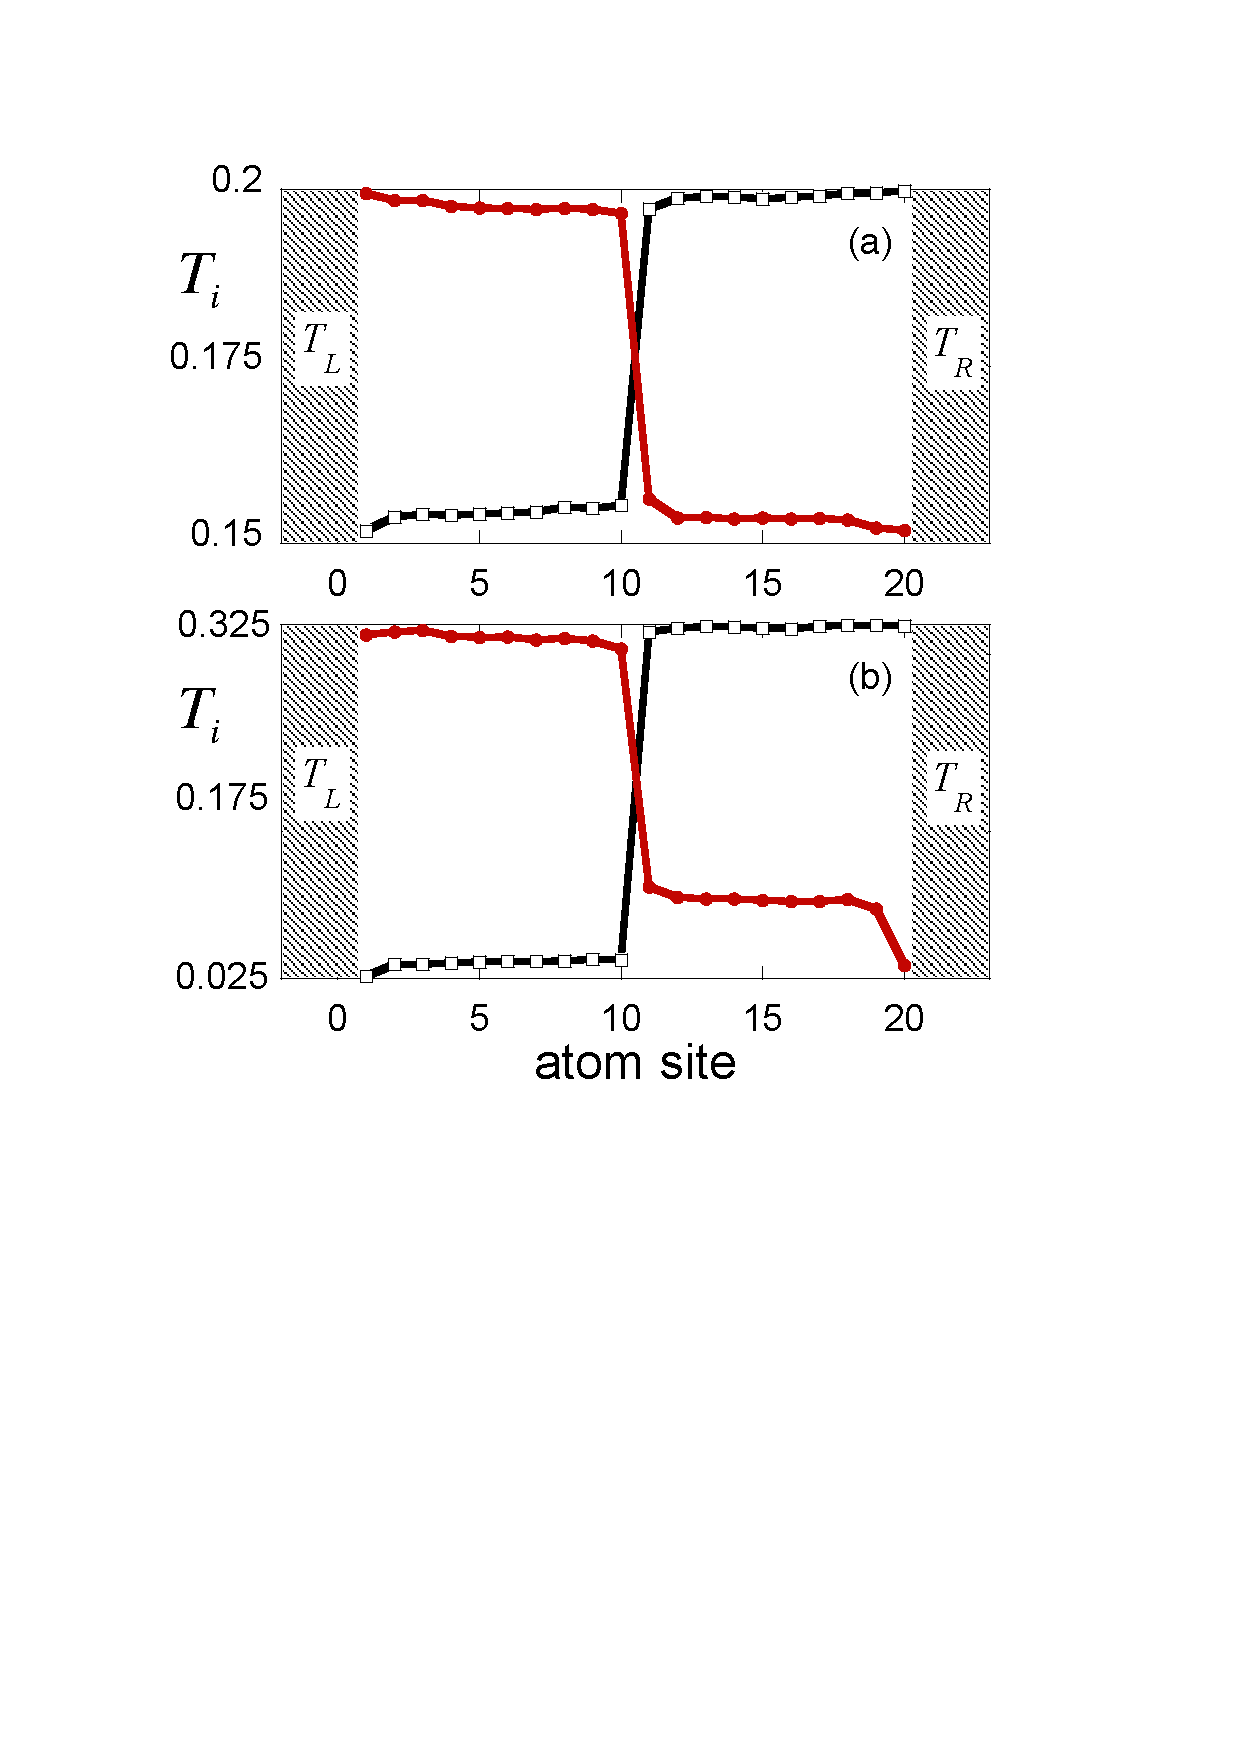
\includegraphics[width=8.8cm]{Figures/FIG6.pdf}
\caption{(Color online) Temperature profile for a harmonic interacting chain of $N=20$ atoms, with an impurity in the $N/2+1$ position, with $T_L=T_h$ and $T_R=T_c$ (circles) and with the thermostat baths switched (squares), for (a) $\Delta T = 0.05$ and (b)  $\Delta T = 0.3$. The corresponding rectification factors are (a) $R=18\%$ and (b) $R=85\%$. Parameters regarding the impurity are the same as in fig. 1.
}
\label{figure6}
\end{figure}

Even though our motivation was to mimic the effect of a localized atom diode that lets atoms pass only one way,
unlike the atom diode \cite{Ruschhaupt2004}, all interactions in the present model
are elastic. The model may be extended by adding an irreversible,  dissipative element so as to induce not only rectification but a truly Maxwell demon for heat transfer \cite{Skordos1992,Ruschhaupt2006}.
On the experimental side, one dimensional chains of neutral atoms in optical lattices can be implemented with cold atoms \cite{Bloch2005}.
An impurity with different internal structure could be subjected to a different on-site potential imprinted by a holographic mask \cite{Bakr2009}, and asymmetrical interatomic interactions
could be implemented by trapping a controllable polar molecule or mediated by atoms in parallel lattices \cite{Gollub2014}.


We are  indebted to G. Casati for raising our attention to thermal rectification and for providing information on his work. We acknowledge financial support by the
Basque Government (Grant No.  IT986-16) and MINECO/FEDER,UE (Grant No. FIS2015-67161-P).
 %Rectification chain of Ions
Reid%!TEX root = ../Thesis.tex
%Chapter 1

\chapter{Chain of Ions}
\label{RectificationChainOfIons}
\lhead{Chapter 1. \emph{Chapter Title}} % Write in your own chapter title to set the page header
%
We numerically demonstrate heat rectification for linear chains of  ions in trap lattices with  graded  trapping frequencies, in contact with
thermal baths implemented by optical molasses.  To calculate the local temperatures and heat currents we find the stationary state
by solving a system of algebraic equations. This approach is much faster than the usual method
that integrates the dynamical equations of the system and averages over noise realizations.
%
\newpage
%
\section{Introduction\label{IntroductionRectificationChainOfIons}}

The ideal thermal rectifier, also ``thermal diode'',  is a device that allows heat to propagate in one direction, from a hot to a cold bath, but not in the opposite one when the temperature bias of the baths is  reversed. The name is set by analogy to the
half-wave rectifiers or diodes for electric current. More generally thermal rectification simply denotes
asymmetric heat flows (not necessarily all or nothing) when the bath temperatures are reversed.
 Thermal rectification was discovered by C. Starr in 1936 in a junction between copper and cuprous oxide \cite{Starr1936}. Many years later, a work of Terraneo \textit{et al.} demonstrated thermal rectification in a model
consisting on a segmented chain of coupled nonlinear oscillators  in contact with two thermal baths at temperatures $T_H$ and $T_C$, with $T_H > T_C$ \cite{Terraneo2002}. This paper sparked a substantial body of research  that spans to this day \cite{Pereira2019} (see Fig. 1 in \cite{Roberts2011}).

\begin{figure*}
    \centering
    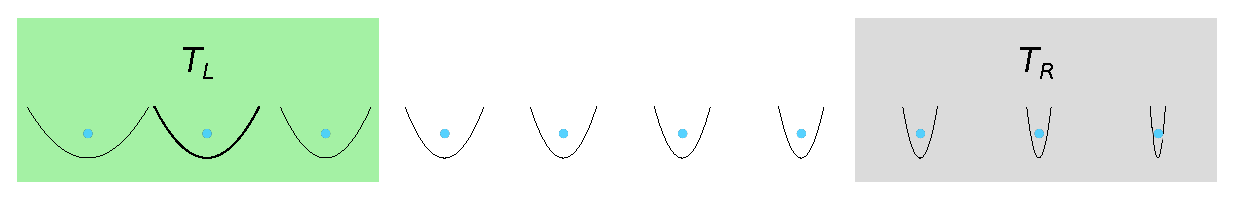
\includegraphics[width=0.9\linewidth]{Figures/Diagram.eps}
    \caption{Schematic representation  of the frequency-graded chain of trapped ions proposed as a thermal rectifier. The left and right ends of the chain are in contact with optical molasses at temperatures $T_L$ and $T_R$ (green and grey boxes respectively). Each ion is in an individual trap. The (angular) frequencies of the traps increase homogeneously from left to right, starting from $\omega_1$ and ending at $\omega_1+\Delta\omega$. The ions interact through the Coulomb force, which is long range, and therefore all the ions interact among them, even distant neighbors. By default  we use 15 ions.}
    \label{fig:Diagram}
\end{figure*}

Research on thermal rectification has gained a lot of attention in recent years as a key ingredient to build
prospective devices to control heat flows similarly to electrical currents \cite{Roberts2011,Li2012}. There are  proposals
%that exploit the analogy with electronic currents
to engineer thermal logic circuits \cite{Ye2017} in which information, stored in thermal memories \cite{Wang2008}, would be processed in thermal gates \cite{Wang2007}. Such thermal gates, as their electronic counterparts,  will require thermal diodes and thermal transistors  to operate \cite{Li2006,Joulain2016}.
%Information may also be stored in thermal memories \cite{Wang2008}.
Heat rectifying devices would also be quite useful  in nano electronic circuits, letting delicate components dissipate heat while being protected from external heat sources \cite{Roberts2011}.

Most work on thermal diodes has been theoretical with only a few experiments \cite{Chang2006,Kobayashi2009,Leitner2013,Elzouka2017}.
A relevant attempt to build a thermal rectifier was based on a graded structure made of carbon and boron nitride nanotubes that transports heat between a pair of heating/sensing circuits \cite{Chang2006}. One of the ends of the nanotube is loaded with a deposition of another material, which makes the heat flow better from the loaded end to the unloaded end. However, rectifications were small, with rectification factors (relative
heat-flow differentials) around $7\%$.
% in \cite{Chang2006}).

Much effort has been aimed at improving the rectification factors and the features of the rectifiers. Some works
relied, as in \cite{Terraneo2002}, on a chain segmented into two or more regions  with different properties,  but using other lattice models such as the Frenkel-Kontorova (FK) model \cite{Li2008,Hu2006}.
The fundamental ingredient for having rectification  was attributed to nonlinear forces in the chain \cite{Zeng2008,Katz2016,Li2008,Hu2006,Benenti2016,Li2012}, which lead to a temperature dependence of the phonon bands or power spectral densities. The bands may match or mismatch at the
interfaces depending on the sign of the temperature bias of the baths, allowing or obstructing heat flow \cite{Terraneo2002,Li2004}.  Later, alternative mechanisms have been
proposed which do not necessarily rely on anharmonic potentials \cite{Pereira2017,Pons2017}.
Also, Peyrard provided a simple model to explain and build rectifiers based on assuming the Fourier law for heat conduction locally
combined with a temperature and position-dependent conductivity \cite{Peyrard2006}.


It was soon realized that the performance of segmented rectifiers was very sensitive to the size of the device, i.e., rectification decreases with increasing the length of the rectifier \cite{Hu2006}. To overcome this limitation two ideas were proposed. The first one consists in using graded rather than segmented chains, i.e., chains where some physical property varies continuously along the site position such as the mass of particles in the lattice \cite{Wang2012,Chen2015,Romero-Bastida2017,Yang2007,Romero-Bastida2013,Dettori2016,Pereira2010,Pereira2011,Avila2013}. The second one uses particles with long-range interactions (LRI), such that all the particles in the lattice interact with each other \cite{Chen2015,Bagchi2017,Pereira2013}. The rationale behind was that in a graded system new asymmetric, rectifying channels are created, while the long-range interactions create
also new transport channels, avoiding the usual decay of heat flow with size \cite{Chen2015}.
%
% ``\textit{with long-range interactions (LRI), we conjecture that the presence of new links (interactions) among different sites creates new channels for the heat transport... Besides that, in a graded system... new asymmetric channels are created which in turn favors the asymmetric flow, i.e., rectification}'' \cite{0295-5075-111-3-30004}.
%
Besides a stronger rectification power, LRI graded chains are expected to have better heat conductivity than segmented ones. This is an important point for technological applications, because devices with high rectification factors are not useful if the currents that flow through them are very small.

In this article we propose to bridge the gap between mathematical models and actual systems
exploring the implementation of a heat rectifier in a realistic, graded system with long-range interactions:
a chain of  ultracold ions in a segmented Paul trap with graded microtraps for each ion.
Long-range interactions are due to the Coulomb forces, and the  baths at the ends of the chain  may be implemented with optical molasses,
see Fig. \ref{fig:Diagram}. The trapping frequencies of the  microtraps are controlled individually in order to create a graded and asymmetric trap-frequency profile along the chain. This asymmetry will lead to a heat flow that depends on the sign of the temperature difference of the baths. Heat transport in trapped ion chains has been studied in several works  \cite{Freitas2015,Ruiz2014,Ruiz2019,Pruttivarasin2011,Ramm2014} and interesting phenomena like phase transitions have been investigated \cite{Freitas2015,Ruiz2014,Ruiz2019,Pruttivarasin2011}. The idea of using locally-controlled traps is already mentioned in \cite{Freitas2015} to implement disorder and study its effects. The device we present here may be challenging to implement, but at reach with the current technology, in particular  that of microfabricated traps \cite{Cirac2000,Krauth2014,Schmied2009}. Thus the setting is thought for a small, realistic number of controllable ions.
% and, while refraining from scaling up the size of the chain beyond realistic
%values, we shall nevertheless analyze  the dependence with the number of ions.

The rest of the article is organized as follows. In Section \ref{Physical System} we describe the physical system of trapped ions with graded trap frequencies. We also set the stochastic dynamics due to the action of lasers at the chain edges.
In Section \ref{sec:HeatFlow}  we implement an efficient  method to find the steady state using Novikov's theorem and solving an algebraic system of equations. In Section \ref{Numerical Results} we present simulations of this system exhibiting thermal rectification and discuss the dependence with ion number, different options for the ion-laser coupling, and the advantages/disadvantages of using a graded frequency profile instead of a segmented one. Finally, in Section \ref{ConclusionsRectificationChainOfIons} we summarize our conclusions, and discuss connections with other works.
%
%
%
\section{Physical System\label{Physical System}}
%
%
%
%
Consider a linear lattice of $N$ individual harmonic traps of (angular) trapping frequencies  $\omega_n$ evenly distributed along the $x$ axis at a distance $a$ from each other. Each trap contains a single ion that interacts with the rest via Coulomb potentials. All the ions are of the same species, with mass $m$ and charge $q$. The Hamiltonian that describes the dynamics of the system is (we consider only linear, one dimensional motion along the chain axis)
%
\begin{equation}
    H(\bm{x},\bm{p}) = \sum_{n=1}^N \left[\frac{p_n^2}{2m}  + \frac{m\omega_n^2}{2} (x_n - x_n^{(0)})^2\right] + V_{int}(\bm{x}),
    \label{eq:ChainHamiltonian}
\end{equation}
%
where $\{x_n,p_n\}$, position and momentum of each ion, are the components of  the vectors
$\bm{x},\bm{p}$, $x_n^{(0)} = n  a$ are the centers of the harmonic traps, and $V_{int}$ is the sum of the Coulomb interaction potential between all  pairs of ions,
%
\begin{equation}
    V_{int}(\bm{x}) = \frac{1}{2}\sum_n \sum_{l\neq n} V_{C}(\left|x_n-x_l\right|),
    \label{eq:InteractionHamiltonian}
\end{equation}
%
with $V_{C}(\left|x_n-x_l\right|) = \frac{q^2}{4\pi\varepsilon_0}\frac{1}{\left|x_n-x_l\right|}$. The ends of the chain are in contact with two thermal reservoirs at temperatures $T_L$ for the left bath and $T_R$ for the right bath respectively. The action of the resevoirs on the dynamics of the chain is modeled via Langevin baths at temperatures $T_L$ and $T_R$ \cite{Lepri2003,Dhar2018}. The equations of motion of the chain, taking into account the baths and the Hamiltonian, are
%
\begin{equation}
    \begin{split}
        \dot{x}_n &= \frac{1}{m}p_n, \\
        \dot{p}_n &= - m\omega_n^2 (x_n-x_n^{(0)}) - \frac{\partial V_{int}}{\partial x_n} - \frac{\gamma_n}{m}p_n + \xi_n(t),
    \end{split}
    \label{eq:Dynamics}
\end{equation}
%
where $\gamma_n$ and $\xi_n(t)$ are only non-zero for the ions in the end regions, in contact with the left and right baths in the sets ${\cal L} = \left\{1,2,...,N_L\right\}$ and ${\cal R} = \left\{N-(N_R-1),...,N-1,N\right\}$,  see Fig. \ref{fig:Diagram}. The $\gamma_n$ are friction coefficients and $\xi_n(t)$ are uncorrelated Gaussian noise forces satisfying $\expval{ \xi_n(t)} = 0$ and $\expval{ \xi_n(t)\xi_m(t') } = 2 D_n \delta_{nm}\delta(t-t')$, $D_n$ being the diffusion coefficients. These Gaussian forces are formally the time derivatives of independent Wiener processes (Brownian motions)   $\xi_n(t) = \sqrt{2D_n}\frac{dW_n}{dt}$ \cite{Toral2014,Ruiz2014} and Eq. \eqref{eq:Dynamics} is a stochastic differential equation (SDE) in the Stratonovich sense \cite{Toral2014}.

The baths are physically implemented by optical molasses consisting of a pair of counterpropagating Doppler-cooling lasers \cite{Ruiz2014}. The friction and diffusion coefficients for the ions in contact with the baths are given by \cite{Cohen1992,Metcalf2003,Ruiz2014}
%
\begin{equation}
    \begin{split}
        \gamma_n &= -4 \hbar k_{L,R}^2 \left(\frac{I_{L,R}}{I_0}\right)\frac{2\delta_{L,R}/\Gamma}{\left[1 + (2\delta_{L,R}/\Gamma)^2\right]^2},\\
        %
        D_n &= \hbar^2 k_{L,R}^2 \left(\frac{I_{L,R}}{I_0}\right) \frac{\Gamma}{1 + (2\delta_{L,R}/\Gamma)^2},\\
        n &\in \cal{L},\cal{R},
    \end{split}
    \label{eq:DopplerCooling}
\end{equation}
%
where $k_L$ ($k_R$) and $I_L$ ($I_R$) are the wave vector and intensity of the left (right) laser. $\delta_L$ ($\delta_R$) is the detuning of the left (right) laser with respect to the angular frequency $\omega_0$ of the atomic transition the laser is exciting, and $\Gamma$ is the corresponding natural line width of the  excited state. The expressions in Eq. \eqref{eq:DopplerCooling} are valid only if the intensities of the lasers are small compared to the saturation intensity $I_0$, $I_{L,R}/I_0\ll 1$. In this bath model, the friction term in Eq. \eqref{eq:Dynamics} comes from the cooling action of the laser and the white noise force $\xi_n(t)$ corresponds to the random recoil of the ions due to spontaneous emission of photons \cite{Metcalf2003,Cohen1992}. Using the diffusion-dissipation relation $D = \gamma k_B T $ \cite{Chee2010}, the temperatures of the optical molasses baths are given by
%
\begin{equation}
    T_{L,R} = -\frac{\hbar \Gamma}{4 k_B} \frac{1+(2\delta_{L,R}/\Gamma)^2}{(2\delta_{L,R}/\Gamma)},
    \label{eq:Doppler}
\end{equation}
%
with $k_B$ being the Boltzmann constant. If the laser intensities are low enough, the temperatures of the baths are controlled by modifying the detunings. When $\delta = \delta_D=-\Gamma / 2$ the optical molasses reach their minimum temperature possible, the Doppler limit $T_{D} = {\hbar \Gamma}/({2k_B})$. Note that away from the Doppler limit the same temperature may be achieved
for two different values of detuning. These two possibilities imply different couplings (two different pairs of $\gamma$ and $D$ values) and thus different physical effects that will be studied in Sec. \ref{TC}.
%
%
%
%
\section{Calculation of the stationary heat currents\label{sec:HeatFlow}}
%
%
The local energy of each site is defined by
%
\begin{equation}
    H_n = \frac{1}{2m} p_n^2 + \frac{1}{2}m\omega_n^2 \left( x_n - x_n^{(0)}\right)^2 +\frac{1}{2}\sum_{l\neq n} V_C(\left|x_n-x_l\right|).
    \label{eq:LocalEnergy}
\end{equation}
%
Differentiating $H_n$ with respect to time we find the continuity  equation
%
\begin{equation}
    \dot{H}_n = \frac{p_n}{m}\! \left[ \xi_n(t)-\gamma_n \frac{p_n}{m} \right]\! - \frac{1}{2m}\!\sum_{l\neq n}\frac{\partial V_C (\left|x_n\!-\!x_l\right|)}{\partial x_n}(p_n + p_l).
    \label{eq:continuityFirst}
\end{equation}
%
Two different contributions can be distinguished: $j^B_n \equiv \frac{p_n}{m} \left[ \xi_n(t)-\gamma_n \frac{p_n}{m} \right]$, which is the energy flow from the laser reservoir to the ions at the edges of the chain (only for $n\in {\cal L}, {\cal R}$), and $\dot{H}_n^{int} \equiv - \frac{1}{2m}\sum_{l\neq n}\frac{\partial V_C (\left|x_n-x_l\right|)}{\partial x_n}(p_n + p_l)$, which gives the ``internal'' energy flow due to the interactions with the rest of the ions. In the steady state $\expval{\dot{H}_n} = 0$, and therefore
%
\begin{equation}
    \expval{j^B_n} + \expval{\dot{H}_n^{int}} = 0,
    \label{eq:continuitySecond}
\end{equation}
%
where $\langle \cdot\!\cdot\!\cdot \rangle$ stands for the expectation value with respect to  the ensemble of noise processes $\bm\xi (t)$ ($\bm\xi$ represents a vector with
components $\xi_n$). Equation \eqref{eq:continuitySecond} implies that, in the steady state, the internal rates $\dot{H}_n^{int}$ vanish for the inner ions of the chain because $j^B_n = 0$ for $n\notin {\cal L},{\cal R}$. In chains with nearest-neighbor (NN) interactions,
$\langle\dot{H}_n^{int}\rangle$ simplifies to two compensating and equal-in-magnitude contributions that define the homogeneous heat flux across the chain.
For long-range interactions this is not so and defining the flux is not so straightforward. A formal possibility is to impose
nearest-neighbor interatomic interactions for some atoms in the chain \cite{Chen2015},
but this approach is not realistic in the current system so we define instead the heat currents
for the left and right baths as
%
\begin{equation}
    \begin{split}
        J_L (t)&= \sum_{n\in {\cal L}} \expval{j^B_n},\\
        J_R (t)&= \sum_{n\in {\cal R}} \expval{j^B_n},
    \end{split}
    \label{eq:BathHeatFlows}
\end{equation}
%
respectively. These expressions are in general time-dependent.
In the steady state we must have $J_{L,{\rm steady}} + J_{R,{\rm steady}} = 0$, since the local energies stabilize and internal energy
flows cancel. We use either $J_{L,{\rm steady}}$ or $J_{R,{\rm steady}}$ to calculate the total energy flow in the chain, always taking the absolute value, i.e., $J \equiv \abs{J_{L,{\rm steady}}}= \abs{J_{R,{\rm steady}}}$. $J$ is defined as $J_\rightarrow$ when the hot bath is on the left
and $J_\leftarrow$ when it is on the right.

To compute the average heat fluxes of the baths $\expval{j^B_n}$ in Eq. \eqref{eq:BathHeatFlows} we need
the averages $\expval{p_n(t)\xi_n(t)}$. Instead of explicitly averaging $p_n(t)\xi_n(t)$ over different realizations of the white noise we use Novikov's theorem \cite{Novikov1965,Ma2011,Toral2014}. Novikov's theorem states that the ensemble average (over  the realizations of the noise) of the product of some functional $\phi(t)$, which depends on a Gaussian noise $\xi(t)$ with zero mean value, $\expval{\xi(t)} = 0$, and the noise itself, is given by
%
\begin{equation}
    \expval{\xi(t)\phi(t)} = \int_0^t dt' \expval{\xi(t)\xi(t')} \expval{\frac{\delta \phi(t)}{\delta\xi(t')}},
    \label{eq:Novikov_GeneralExpression}
\end{equation}
%
where ${\delta \phi(t)}/{\delta\xi(t')}$ is the functional derivative of $\phi(t)$ with respect to the noise, with $t'<t$. When the noise is $\delta-$correlated, $\expval{\xi(t)\xi(t')}=2D\delta(t-t')$, and Eq. \eqref{eq:Novikov_GeneralExpression} reads $\expval{\xi(t)\phi(t)} = D \expval{{\delta \phi(t)}/{\delta\xi(t')}}|_{t' \to t^-}$. To apply Novikov's theorem to our model we need the functional derivatives of the position $x_n(t)$ and momentum $p_n(t)$ coordinates with respect to the white noises. We integrate Eq. \eqref{eq:Dynamics} to have its formal solution as a functional depending on the white Gaussian noises $\xi_n(t)$,
%
\begin{equation}
    \begin{split}
        x_n(t) &= x_n(0) +  \frac{1}{m}\int_0^t ds\; p_n(s) ,\\
        p_n(t) &= p_n(0) + \int_0^t ds\; \left[ -\frac{\partial H}{\partial x_n}(s) - \frac{\gamma_n}{m}p_n(s) + \xi_n(s)\right].
    \end{split}
    \label{eq:FormalSolution}
\end{equation}
%
Equation \eqref{eq:FormalSolution} implies that the functional derivatives are ${\delta x_n(t)}/{\delta \xi_m(t')}|_{t'\to t^-} = 0$ and
${\delta p_n(t)}/{\delta \xi_m(t')}|_{t'\to t^-} = \delta_{nm}$ ($\delta_{nm}$ is the usual Kronecker delta symbol). Thus we have $\expval{x_n(t) \xi_m(t)} = 0$ and $\expval{p_n(t) \xi_m(t)} = \delta_{nm}D_m$, which gives for the heat flow from the baths
%
\begin{equation}
    \expval{j^B_n} = \frac{1}{m} \left[ D_n-\gamma_n \frac{\expval{p_n^2}}{m} \right].
\end{equation}
%
In all simulations we check that $|J_{L,{\rm steady}}|=|J_{R,{\rm steady}}|$ within the numerical tolerance of the computer. To measure the asymmetry of the heat currents we use the rectification factor $R$ defined as
%
\begin{equation}
    R = \frac{ J_\rightarrow - J_\leftarrow}{max(J_\rightarrow,J_\leftarrow)}.
    \label{eq:R_Factor}
\end{equation}
%
$R$ values may go from $-1$ to $1$ (In the figures we depict it in \% between -100\% and 100\%). If there is no rectification $J_\rightarrow = J_\leftarrow $ and $R=0$. For perfect rectification in the right (left) direction, $J_\rightarrow \gg J_\leftarrow$ ($J_\rightarrow \ll J_\leftarrow$), and $R = 1$ ($R = -1$).
Take note that other  definitions of rectification factors exist in many works
on asymmetric heat transfer so comparisons should be done with care.
%

This model does not show the antithermodynamical behavior  observed in other models
\cite{De-Chiara2018,Levy2014}, and heat is found to flow in all cases from the hot to the
cold bath.
% blue{The Langevin bath is known to be equivalent to a local master equation, which can give thermodynamical inconsistencies . However, we have not observed any violation of the first and second laws of thermodynamics in our simulations, since the system reaches a steady state where the incoming and outcoming heat currents compensate each other and heat always flows from the hot to the cold bath.}%
%
%
%
\subsection{Algebraic, small-oscillations approach to calculate the steady state\label{steadyState}}
%
%
%
%
To find the temperature profiles and heat currents in the steady state the usual approach is to solve the SDE system in Eq. \eqref{eq:Dynamics} up to long times  and for many realizations of the white noises $\bm\xi (t)$. In that way the ensemble averages $\expval{p_n(t \to \infty)^2}$, necessary for both the temperature profiles and heat currents, are computed. This standard route implies a heavy computational effort, in particular  when we want to study the heat transport for several bath configurations, frequency increments and chain parameters. It is possible to circumvent this difficulty and find ensemble averages like $\expval{x_n x_m}$, $\expval{x_n p_m}$, $\expval{p_n p_m}$ (second order moments) without integrating any SDE \cite{Sarkka2019}. The idea is to impose the condition ${d\expval{\cdot\cdot\cdot}}/{dt} = 0$ for all the second order moments and linearize the dynamical equations of the system around equilibrium.
A system of linear algebraic equations for the moments results, that can be easily solved without solving the SDE many times.
% to solve a system of linear algebraic equations. We will analyze the validity of the linearized approximation in the following section.


To linearize the SDE in Eq. \eqref{eq:Dynamics} we approximate the potential energy of the Hamiltonian in Eq. \eqref{eq:ChainHamiltonian}, $V(\bm{x}) = V_{int}(\bm{x}) + m\;\sum_n \omega_n^2 (x_n-x_n^{(0)})^2/2$, by its harmonic approximation around the equilibrium positions $\bm{x}^{eq}$, defined by  $\frac{\partial V(\bm{x})}{\partial\bm{x}}\Big|_{\bm{x}=\bm{x}^{eq}} = 0$. The approximate potential (ignoring the zero-point energy) is
%
\begin{equation}
    V(\bm{x})\approx  \frac{1}{2} \sum_{n,m} K_{nm} (x_n-x_n^{eq})(x_m-x_m^{eq}),
\end{equation}
%
with $K_{nm} = \frac{\partial^2 V(\bm{x})}{\partial x_n \partial x_m}\Big|_{\bm{x}=\bm{x}^{eq}}$ being the Hessian matrix entries of $V(\bm{x})$ around the equilibrium configuration \cite{James1998}
%
\begin{equation}
    K_{nm} =
    \begin{cases}
        m \omega_n^2 + 2 \left(\frac{q^2}{4\pi\varepsilon_0}\right) \sum_{l \neq n  }\frac{1}{\left|x_n^{eq}-x_l^{eq}\right|^3} & \text{if  } n=m\\

         - 2 \left(\frac{q^2}{4\pi\varepsilon_0}\right) \frac{1}{\left|x_n^{eq}-x_m^{eq}\right|^3} & \text{if  } n \neq m
    \end{cases}.
\end{equation}
%
Note that this approximation does not modify the two main features of the system, namely asymmetry and long-range interactions, which are manifest in the asymmetric distribution of $\omega_n$ and the non-zero off-diagonal elements of the $K$ matrix, respectively. In the following we will use $y_n=x_n-x_n^{eq}$ to simplify the notation. The linearized dynamics around the equilibrium positions are given by
%
\begin{equation}
    \begin{split}
        \dot{y}_n &= \frac{1}{m}p_n,\\
        \dot{p}_n &= -\sum_{l}K_{nl}y_l- \frac{\gamma_n}{m}p_n + \xi_n(t).
    \end{split}
    \label{eq:DynamicsHarmonic}
\end{equation}
%
Now, we set ${d\expval{\cdot\!\cdot\!\cdot}}/{dt} = 0$ for all the moments. Using Eq. \eqref{eq:DynamicsHarmonic} and applying Novikov's theorem we find
%
% \begin{widetext}
% \begin{eqnarray}
%     \frac{d}{dt}(x_n x_l) &=& \frac{1}{m}(x_n p_l + x_l p_n) , \nonumber\\
%     \frac{d}{dt}(x_n p_l) &=& \frac{1}{m}\left(p_n p_l - \gamma_l x_n p_l\right) - \sum_m K_{lm}x_n x_m + x_n \xi_l , \nonumber\\
%     \frac{d}{dt}(p_n p_l) &=& - \sum_m x_m\left( K_{nm}p_l + K_{lm} p_n \right) - \frac{1}{m}(\gamma_l + \gamma_n) p_n p_l + \xi_n p_l + \xi_l p_n .
% \label{eq:DynamicsHarmonicOfMomenta}
% \end{eqnarray}
% \end{widetext}
%
% Now we make use of $\frac{d\expval{}}{dt} = 0$ and the Novikov theorem \cite{1965JETP20.1290N,PhysRevB.83.134418}, which in this case implies $\expval{ x_n \xi_l } = 0 $ and $\expval{ p_n \xi_l } = \delta_{nl}D_n$, to finally find
%
\begin{equation}
    \begin{split}
        \expval{p_n p_l} - \gamma_l\expval{y_n p_l} - \sum_m K_{lm}\expval{y_n y_m} &= 0,\\
        \sum_{m}\left[ K_{nm}\expval{y_m p_l} + K_{lm}\expval{y_m p_n} \right] + \frac{1}{m}\left( \gamma_l + \gamma_n \right)\expval{p_n p_l} &= 2 \delta_{nl} D_n.
    \end{split}
    \label{eq:SteadyStateEquation}
\end{equation}
%
The system \eqref{eq:SteadyStateEquation} is linear in the second order moments so it can be solved numerically to find the steady-state values of the moments. Besides Eq. \eqref{eq:SteadyStateEquation} we have that $\expval{y_n p_l} = - \expval{y_l p_n}$, which follows from Eq. \eqref{eq:DynamicsHarmonic} and $d\expval{y_n y_m}/dt = 0$. Since there are $\frac{1}{2}N(N-1)$ independent $\expval{y_n p_l}$ moments, we choose the ones with $n<l$. Similarly, the moments $\expval{y_n y_l}$ and $\expval{p_n p_l}$ contribute with $\frac{1}{2}N(N+1)$ independent variables each and we choose the ones with $n\leq m$. Thus there are in total $\frac{1}{2}N(3N+1)$ independent moments that we arrange in the vector
%
\begin{equation}
\begin{split}
    \bm\eta = \Big[ &\expval{y_1 y_1},\expval{y_1 y_2},...,\expval{y_N y_N},\\
    &\expval{p_1 p_1},\expval{p_1 p_2},...,\expval{p_N p_N},\\
    &\expval{y_1 p_2},\expval{y_1 p_3},...,\expval{y_{N-1} p_N}\Big]^T.
    \label{eq:CovariancesVector}
\end{split}
\end{equation}
%
There are the same number of independent equations
%in Eq. \eqref{eq:SteadyStateEquation}
as independent moments: $N^2$
equations correspond to the first line in Eq.  \eqref{eq:SteadyStateEquation}, and $\frac{1}{2}N(N+1)$ equations
to the second line because of the symmetry with respect to $n,l$. The system of equations \eqref{eq:SteadyStateEquation} may be compactly written as $\mathbf{A}\boldsymbol\eta = \mathbf{B}$, where $\mathbf{A}$ and $\mathbf{B}$ are a $\frac{1}{2}N(3N+1)$ square matrix and vector.
% which are built by rearranging the coefficients in the left and right hand sizes of \eqref{eq:SteadyStateEquation} in the appropiate way.
%
%
%
%
%
\section{Numerical Results\label{Numerical Results}}
%
%
%
%
%
\begin{figure}[h]
    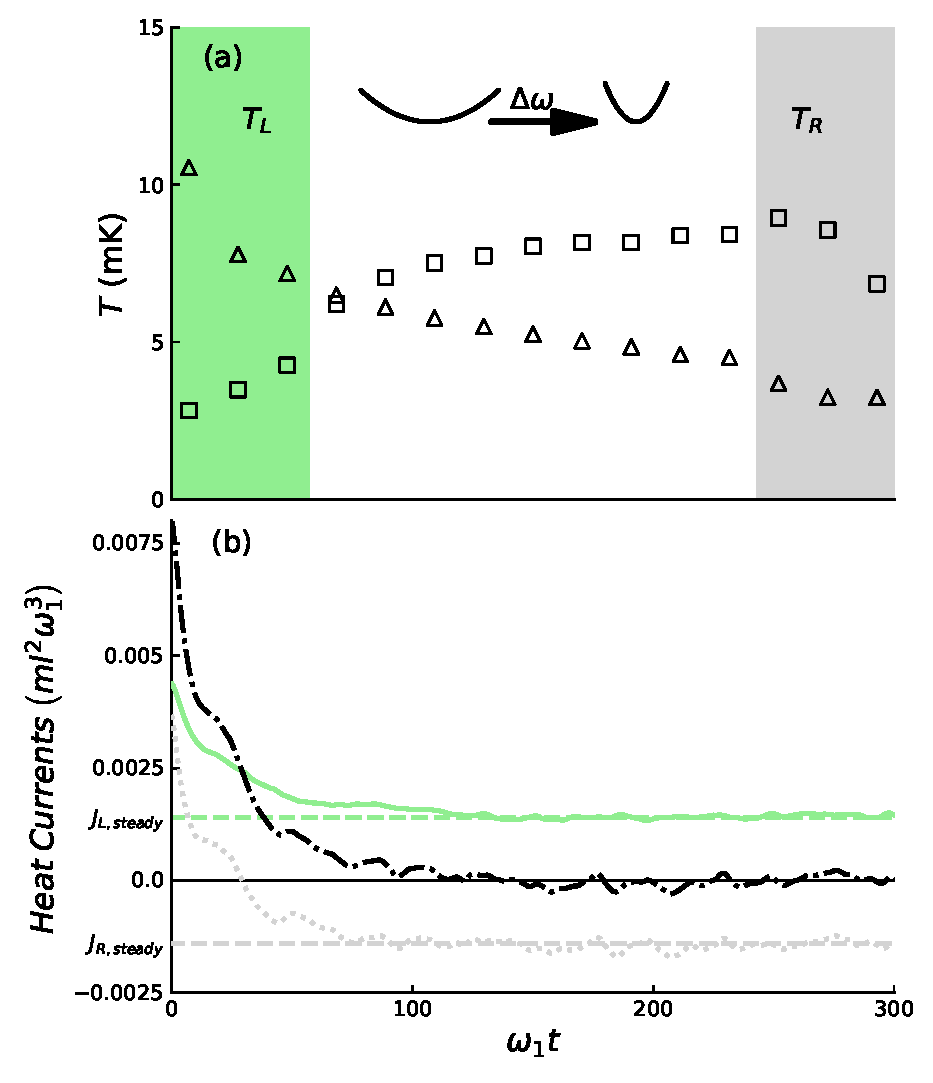
\includegraphics[width=\linewidth]{Figures/24Mg_Temperature_Profiles_And_Evolution.eps}
 \caption{(a) Temperatures of the ions in the stationary state for a graded chain with the parameters described in section \ref{Results_A}. The temperature profiles found with the algebraic method (Eq. \eqref{eq:SteadyStateEquation}) are indistinguishable from the ones found solving the Langevin equation (Eq. \eqref{eq:Dynamics}). Empty triangles (squares) correspond to $T_L = T_H$ ($T_L = T_C$) and $T_R = T_C$ ($T_R = T_H$). (b) Heat currents  as a function of time for $T_L = T_H$ and $T_R = T_C$, see Eq. (\ref{eq:BathHeatFlows}): $J_L(t)$ (solid green line) from the left reservoir into the chain;
 $J_R(t)$ (dotted grey line) from the right reservoir into the chain (negative except at very short times); $J_L(t)+J_R(t)$
 (dotted-dashed black line), which must go to zero in the steady state. The three lines tend to stationary values marked by horizontal lines. Parameters: $\omega_1 = 2\pi \times 50$ kHz,
$a=50\, \mu$m,  $\delta_H = -0.02 \, \Gamma$, and $\delta_C = -0.1 \, \Gamma$, which gives temperatures $T_H \approx 12$ mK and $T_C \approx 3$ mK. $\Delta\omega = 0.5 \, \omega_1$. In all figures $\Gamma = 2\pi \times 41.3$ MHz.}
    \label{fig:Temperature_Profiles_Magnesium}
\end{figure}

We now display the results of our simulations. To find the temperature profiles and the currents in the steady state we use the algebraic method described in section \ref{steadyState}. We also check that the results coincide with those by solving Eq. \eqref{eq:Dynamics} for many different realizations of the noisy forces $\bm\xi (t)$ and averaging. The code for all the numerical simulations has been written in the language \textit{Julia} \cite{Bezanson2012,Bezanson2017}. In particular, to solve the Langevin equation, we used \textit{Julia}'s package \textit{DifferentialEquations.jl} \cite{Rackauckas2017}.

To model the baths and the chain we use atomic data taken from ion trap experiments \cite{Leupold2015,Lo2015}. We consider 15 $^{24}$Mg$^+$ ions in all figures except in Fig. \ref{fig:N_Dependence}. The three leftmost and three rightmost ions are illuminated by Doppler cooling lasers. The Doppler cooling lasers excite the transition $3s^2S_{1/2}\rightarrow 3p^2P_{1/2}$, with angular frequency $\omega_0 = 2 \pi \times 1069$ THz and excited state line width $\Gamma = 2\pi \times 41.3$ MHz \cite{Ruiz2014}. For this ionic species and atomic transition the Doppler limit is $T_D = 1$ mK.
%We use typical trap frequencies of the order of MegaHertzs and intertrap spacings of a few tens of $\mu$m.
The intensities of the laser beams are small compared to the saturation intensity $I_0$ so that Eq. \eqref{eq:DopplerCooling} holds. We take $I_n/I_0 = 0.08$ for the ions  in the laser beams, whereas  $I_n=0$ for the rest.

The temperatures $T_L,\,T_R$ of the left and right laser baths are controlled with their detunings $\delta_L,\,\delta_R$ with respect to the atomic transition. We fix two values for the detunings, $\delta_H$ and $\delta_C$, such that $T_H>T_C$ (hot and cold baths, also source and drain) and we define $J_\rightarrow$ ($J_\leftarrow$) as the stationary heat current in the chain when $T_L = T_H$ and $T_R = T_C$ ($T_L = T_C$ and $T_R = T_H$).

Except in Sec. \ref{GS} we consider a graded frequency profile.
%In the graded chain the frequency increases by $\frac{\Delta\omega}{N-1}$ from one trap to the next.
If the frequency of the leftmost trap is $\omega_1$, the frequency of the $n$th trap will be $\omega_n = \omega_1 +\Delta\omega\frac{n-1}{N-1}$ up to $\omega_1 +\Delta\omega$ for the rightmost trap. In
Sec. \ref{GS} we compare the graded chain to a segmented chain, where the left half of the chain has trapping frequencies $\omega_1$ while the other half has $\omega_1 +\Delta\omega$.


\subsection{Evolution to steady state \label{Results_A}}

\begin{figure}[h]
    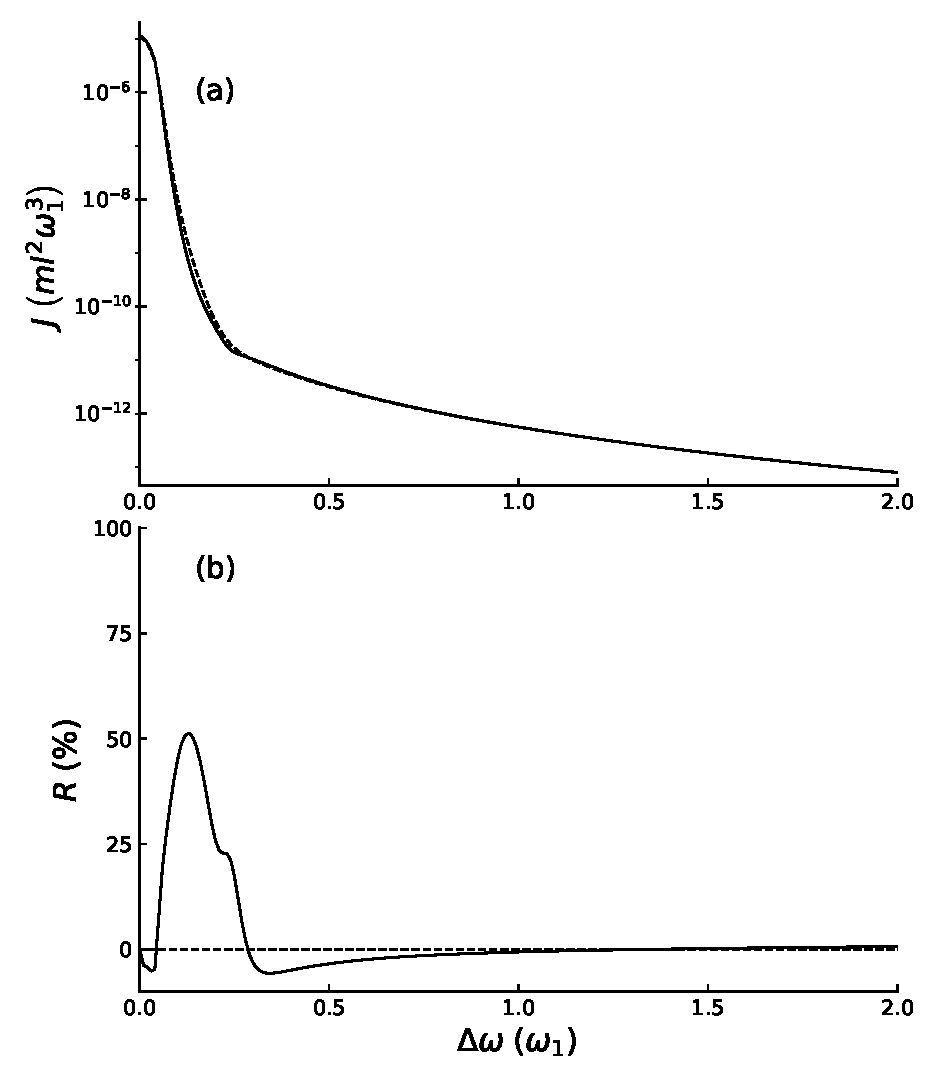
\includegraphics[width=\linewidth]{Figures/Graded_24Mg_FluxAndRectification_VS_FreqGradient.eps}
    \caption{Graded chain of $N=15$ $^{24}$Mg$^+$ ions. (a) Stationary fluxes for different frequency increments:
$J_\rightarrow$   (for $T_L = T_H$ and $T_R = T_C$, dashed line); $J_\leftarrow$ (for $T_L = T_C$ and $T_R = T_H$, solid line)
(b) Rectification factor. Parameters: $\omega_1 = 2 \pi \times 1$ MHz, $l = 5.25\;\mu$m, $a = 4.76\, l$ ($25\,\mu$m), $\delta_H = -0.02 \,\Gamma$, and $\delta_C = -0.1 \, \Gamma$.}
    \label{fig:RFG}
\end{figure}

To compare the results by solving Eq. \eqref{eq:Dynamics} and averaging and those from the algebraic method we  simulated a frequency graded chain with a trapping frequency $\omega_1 = 2\pi \times 50$ kHz for the leftmost ion, see Fig. \ref{fig:Temperature_Profiles_Magnesium}.  The number of ions interacting with the laser beams (three on each bath) is consistent with the lattice constant and typical waists of Gaussian laser beams \cite{Leupold2015,Lo2015}. To set the trap distance we fix first the characteristic length  $l =  \left(\frac{q^2}{4\pi\varepsilon_0}\frac{1}{m\omega_1^2}\right)^{1/3}$ as the distance for which the Coulomb repulsion of two ions equals the trap  potential energy for an ion at a distance
$l$ away from the center of its trap.
If $a<l$, the Coulomb repulsion of the ions is stronger than the trap confinement which makes the ions jump from their traps. With the parameters used in this section we have $l = 38.7\,\mu$m and set $a = 1.29 \,l=50\,\mu$m. The detunings of the \textit{hot} and \textit{cold} lasers are $\delta_H = -0.02 \, \Gamma$, and $\delta_C = -0.1 \, \Gamma$ which gives temperatures $T_H \approx 12$ mK and $T_C \approx 3$ mK. We fix the value $\Delta\omega = 0.5 \, \omega_1$ for the frequency increment.

The results of the two methods are in very good agreement. In the scale of Fig. \ref{fig:Temperature_Profiles_Magnesium} (a)
the calculated local temperatures are undistinguishable. In the calculation based on solving the dynamics we had to integrate Eq. \eqref{eq:Dynamics} for $N_{trials} = 1000$ realizations of white noise $\bm{\xi}(t)$. The method based on the system of moments
shortened the calculation time with respect to the dynamical trajectories   by a factor of $1/700$. In fact, the time gain is even more important because
the dynamical method requires further processing, performing a time averaging to compute the stationary flux in addition to noise averaging, see Fig.  \ref{fig:Temperature_Profiles_Magnesium} (b).


Additionally, the relaxation to the steady state slows down when the frequencies of the traps increase since the deterministic part of the Langevin equation dominates the dynamics over the stochastic part, entering an under-damped regime. In contrast, this increase does not affect the
algebraic method.
%%%%%%%%%%%%%%%%%%%%
\begin{figure}[t]
    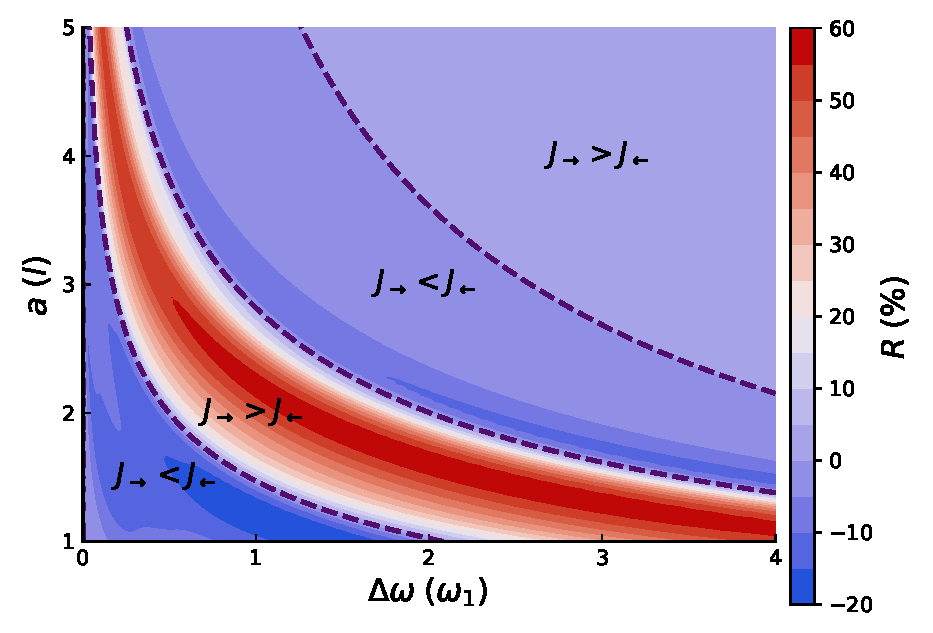
\includegraphics[width=\linewidth]{Figures/Graded_24Mg_Rectification_VS_Gradient_and_lattConstant.eps}
    \caption{ Rectification factor in a graded chain of $N=15$ $^{24}$Mg$^+$ ions for different trap distances and frequency increment. The dashed lines are for $R = 0$ and delimit the regions $J_\rightarrow > J_\leftarrow$ and $J_\rightarrow < J_\leftarrow$. The parameters  are $\omega_1 = 2 \pi \times 1$ MHz, $l = 5.25\,\mu$m, $\delta_H = -0.02 \,\Gamma$, and $\delta_C = -0.1 \, \Gamma$.}
    \label{fig:Graded_24Mg_Rectification_VS_Gradient_and_lattConstant}
\end{figure}
%
%
%
%
\subsection{Rectification in frequency graded chains \label{GradedChains}}
%
%
\begin{figure}
    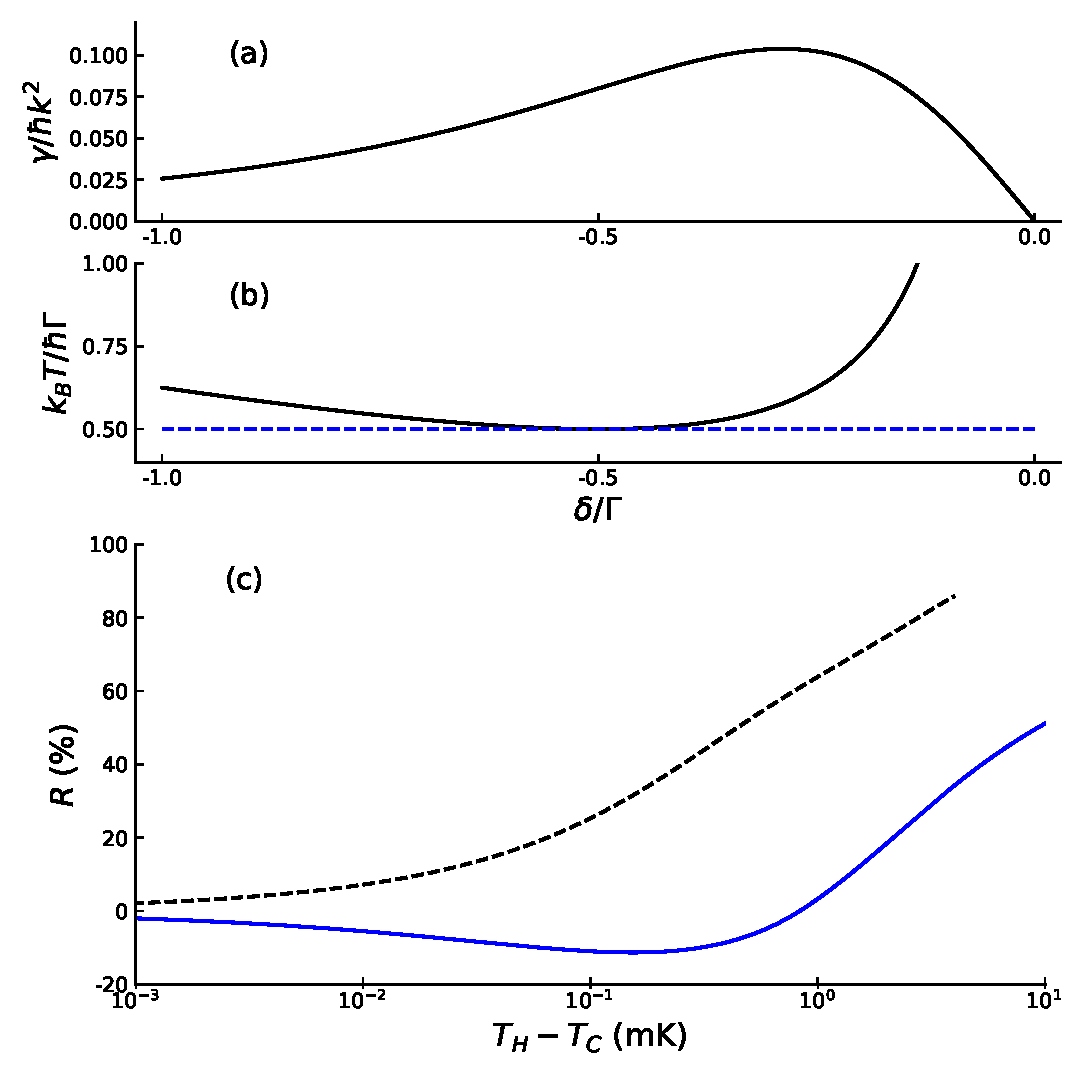
\includegraphics[width=\linewidth]{Figures/R_as_function_of_TemperatureBias.eps}
    \caption{ (a) Friction coefficient defined in Eq. \eqref{eq:DopplerCooling}. (b) Bath temperature defined in Eq. \eqref{eq:Doppler}. (c) Rectification as a function of the temperature difference between the hot and cold baths $T_H -T_C$ for $\delta_H$ below (dashed black line) and above (solid blue line) the Doppler limit, and $\delta_C=\delta_D$ (Doppler limit). Parameters: $\omega_1 = 2 \pi \times 1$ MHz, $\Delta \omega = 0.15 \, \omega_1$, $l = 5.25\,\mu$m, $a = 4.76 \, l$.}
    \label{fig:RD}
\end{figure}
%
In this subsection we demonstrate rectification for the frequency graded chain. We  used the method described in section \ref{steadyState} for $^{24}$Mg$^+$ ions with the same parameters for the baths used before. We fix the trapping frequency of the leftmost trap to $\omega_1 = 2\pi \times 1$ MHz, and a trap spacing $a = 4.76\, l$ ($25\,\mu$m) (the  characteristic length is $l = 5.25\,\mu$m). Figure \ref{fig:RFG} depicts  the results with these parameters in a graded chain. Figure \ref{fig:RFG} (a) shows that both
$J_\rightarrow$ and $J_\leftarrow$
% the right-going flux (dashed line) and the left-going flux (solid line)
decrease rapidly as the frequency increment  is increased.
%In Fig. \ref{fig:Graded_24Mg_FluxAndRectification_VS_FreqGradient} we see that
The rectification reaches its maximum value for a frequency difference of $\Delta\omega \approx 0.1 \omega_1$. The fluxes cross so there are some points where the rectification is exactly zero, besides the trivial one at $\Delta\omega = 0$, at $\Delta\omega = 0.05\,\omega_1,\;0.3\,\omega_1,\;1.3\,\omega_1$. At these points the direction of rectification reverses, presumably as a consequence of the changes in the match/mismatch of the temperature dependent local power spectra.
The change of rectification direction occurs for all the choices of parameters, as displayed in Fig. \ref{fig:Graded_24Mg_Rectification_VS_Gradient_and_lattConstant}. Figure \ref{fig:Graded_24Mg_Rectification_VS_Gradient_and_lattConstant} gives the rectification factor for different trap distances and frequency increments.  $0$-rectification curves separate regions with different rectification direction. The second region in Fig. \ref{fig:Graded_24Mg_Rectification_VS_Gradient_and_lattConstant} (starting from the left) would be the most interesting one to build a thermal diode, since rectification reaches its largest values there.

{For small values of $\Delta \omega$ there is little asymmetry in the chain and therefore modest rectification is expected whereas a very large $\Delta \omega$ implies very high trapping frequencies on the right implying too strong a
confinement and vanishing interactions. This bottleneck decreases the fluxes in both directions and  the rectification. However, since $\Delta \omega$ is controllable,
and the range of values of $\Delta \omega$ for which rectification is larger can be also controlled with the intertrap distance $a$, see Fig. \ref{fig:Graded_24Mg_Rectification_VS_Gradient_and_lattConstant},
the existence of a rectification window
does not imply a major limitation.}

\begin{figure}
    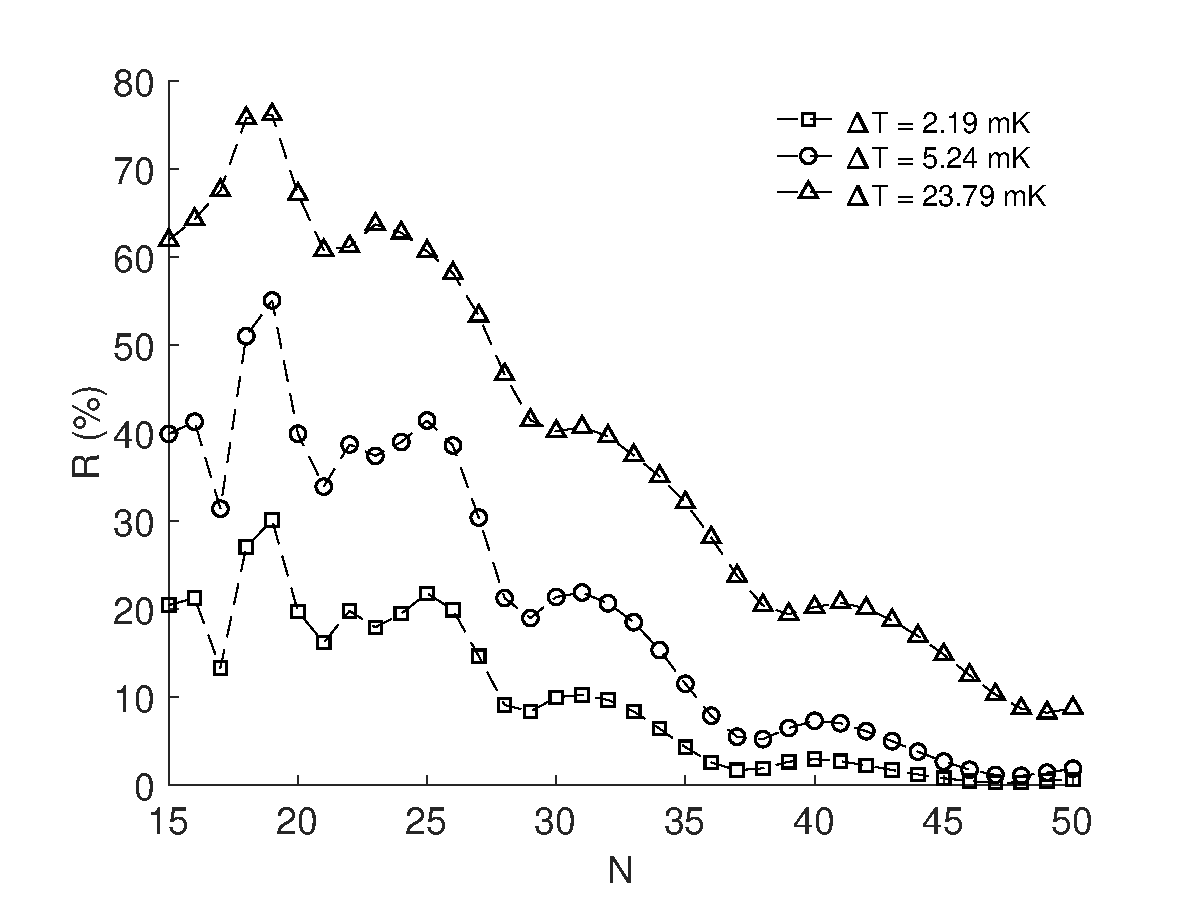
\includegraphics[width=\linewidth]{Figures/Changing_N.eps}
    \caption{Rectification factor for different bath temperature differences $\Delta T$ as the number of ions is increased. The detuning of the cold bath laser is set to the Doppler limit $\delta_C = - \Gamma / 2$. $\omega_1 = 2 \pi \times 1$ MHz, $\Delta \omega = 0.15 \, \omega_1$, $l = 5.25\,\mu$m, $a = 4.76 \, l$.}
    \label{fig:N_Dependence}
\end{figure}
%
%
\subsection{Same bath temperatures, different bath couplings\label{TC}}
%
%
As already mentioned below Eq. (\ref{eq:Doppler}), above and below the detuning  $\delta_D=-\Gamma/2$ corresponding to the  Doppler limit temperature, the optical molasses allow for
two different couplings (two pairs of friction and diffusion coefficients in Eq. (\ref{eq:DopplerCooling})) between the ions and the laser corresponding to the same bath temperature.
This duality may be seen explicitly in Fig. \ref{fig:RD}. Specifically Fig. \ref{fig:RD} (a) depicts the variation of the friction coefficient for values of $\delta$ around $\delta_R$,  and Fig. \ref{fig:RD} (b) the corresponding temperatures.
Interestingly, the different couplings imply different rectification factors.
% To check if this requirement is fulfilled we have calculated the rectification factor for different temperatures in the baths.
If we set $\delta_C = \delta_D=-\Gamma / 2$,  i.e., the cold bath is cooled to the Doppler limit, $\delta_H$ can be chosen to be below or above $\delta_D$ for the same temperature $T_H$. The corresponding rectification factors for the two choices
are shown in  Fig. \ref{fig:RD} (c),
%We see that it is possible to achieve comparable rectifications for smaller temperature differences when $\delta_H<\delta_D$.
%Note that since the effective laser temperatures depend on the linewidth $\Gamma$ of the atomic transition, the range of temperatures that can be reached is limited to the mK. Although other works have shown rectification in temperatures of the order of 100 K \cite{Elzouka2017}, the nature of the rectification mechanism and the physical system are very different. Here we have considered an atomic system, instead of a macroscopic one, where the temperatures are intrinsically low.
which
demonstrates that significant rectification can be achieved by choosing $\delta_H<\delta_D$ for temperature increments that
are smaller than or of the order of $T_C=T_D$, for example $R\approx 20\%$ for $\Delta T=0.1 T_C$, or $R\approx 60\%$
for $\Delta T= T_C$.  Finding good rectification at low (relative) temperature differences is considered to be one on the challenges
in asymmetric heat transport research \cite{Zhang2015}.


%. The temperature of the hot bath is controlled by changing the detuning of its laser. Any detuning we choose for the hot bath is going to give a larger temperature, since the cold one is already set to the minimum posible value at the Doppler limit. We can do this by setting a detuning below ($\delta_H < -\Gamma / 2$) or above ($\delta_H > -\Gamma / 2$) the Doppler limit for the hot bath, see Fig. \ref{fig:RD} (b). The dynamics of the chain will be different for the same temperature bias depending if the detuning of the hot bath is below or above the Doppler limit because the corresponding friction coefficients will be different, see Fig. \ref{fig:RD} (a). As a consequence, different currents and rectifications will be found in the chain depending if $\delta_H$ is below or above the Doppler limit. In Fig. \ref{fig:RFG} maximum rectification values are around $60 \,\%$ with temperature differences of around 10 mK. This temperature difference is roughly four times the temperature of the cold bath, so it is a relatively high temperature difference. Thus, in principle, it looks that high temperature differences are needed to obtain rectification. However, this is not always the case.
%
%
%
\subsection{Dependence with ion number\label{IN}}
%
Keeping in mind that scaling the frequency-graded ion chain  to a large numbers of ions is not a realistic option in this setting,
it is nevertheless important to
study the dependence with ion number from small to moderate numbers.  In Fig. \ref{fig:N_Dependence} we observe an overall trend in which the rectification decreases with the number of ions in the chain (while it increases with temperature bias $\Delta T$ in the studied range). This effect is easy to understand, as increasing $N$
while keeping the total variation of the trapping frequency $\Delta \omega$ constant, the frequency gradient  decreases. This
lowers  the  asymmetry in the chain and the rectification factor. Oscillations with $N$ superimposed to the global trend are more visible at the smaller $N$ values giving  an optimal $N$ value at $N=19$.

\subsection{Graded versus segmented\label{GS}}
%
We have also compared the performance of the graded thermal diode and a segmented version in which the left half of the chain is trapped with frequency $\omega_1$ and the right half (including the middle ion) with $\omega_1+\Delta \omega$. Even though the optimal rectification  in Fig. \ref{fig:GS} (a)  for the segmented chain is larger than for the graded chain, the fact that the fluxes are generally much larger for the graded chain, see Fig. \ref{fig:GS} (b), makes the graded chain more interesting for applications.



\begin{figure}[t]
    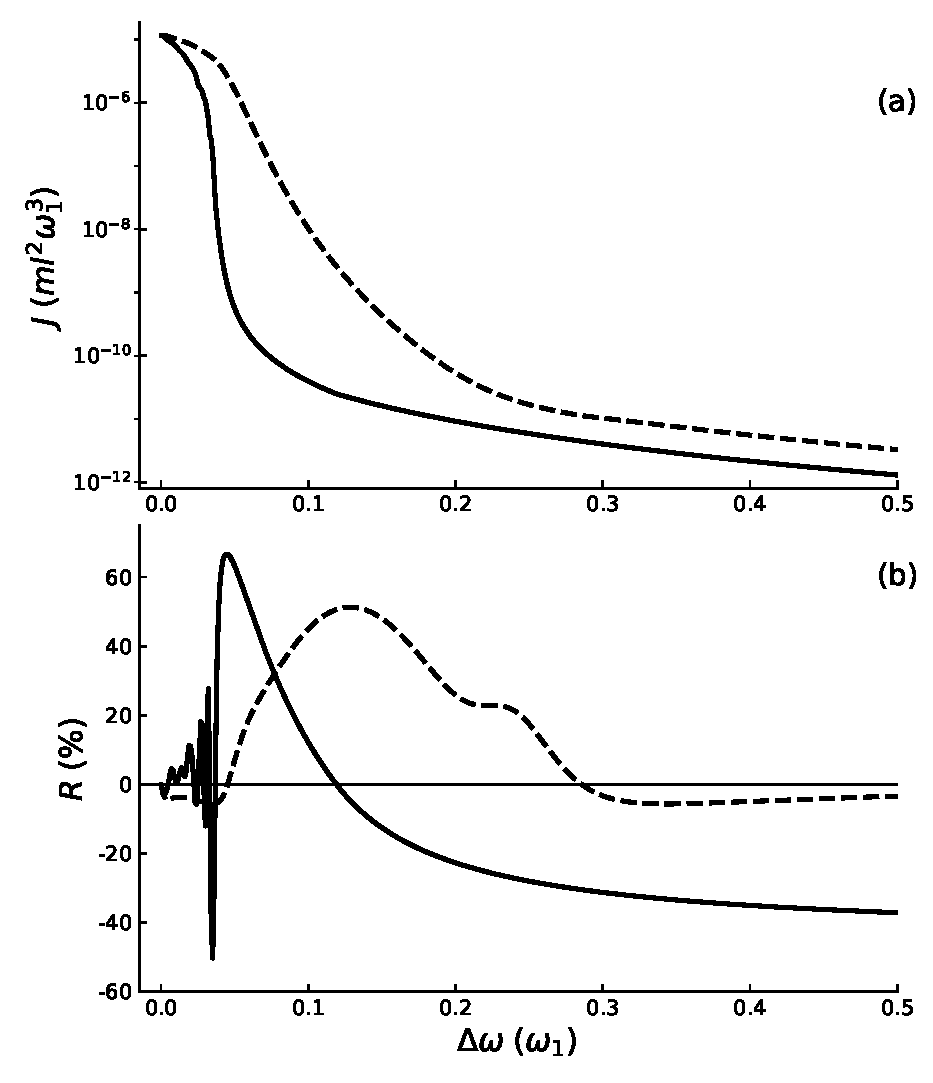
\includegraphics[width=\linewidth]{Figures/24Mg_Comparacion_Graded_AND_Segmented.eps}
    \caption{Comparison of graded and segmented chains with $N=15$ $^{24}$Mg$^+$ ions. (a) Maximum
    of $J_\rightarrow$ and $J_\leftarrow$
     for the graded and segmented chain for different frequency increments. (b) Rectification factor: graded chain (dashed lines); segmented chain (solid lines). Parameters: $\omega_1 = 2 \pi \times 1$ MHz, $l = 5.25\,\mu$m, $a = 4.76 \, l$, $\delta_H = -0.02 \, \Gamma$, and $\delta_C = -0.1 \, \Gamma$.}
    \label{fig:GS}
\end{figure}





\begin{figure}[t]
    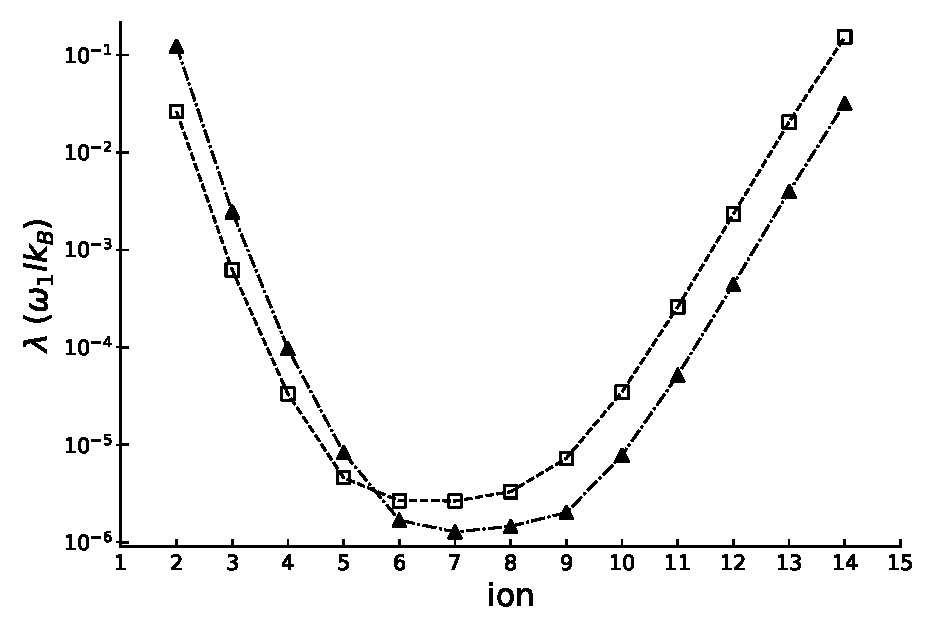
\includegraphics[width=\linewidth]{Figures/fig_lambda_centered.eps}
    \caption{Thermal conductivity through the chain for $T_L > T_R$ (empty squares), and $T_L < T_R$ (filled triangles). $\omega_1 = 2 \pi \times 1$ MHz, $\Delta \omega = 0.15 \, \omega_1$, $l = 5.25\,\mu$m, $a = 4.76 \, l$, $\delta_H = -0.02 \,\Gamma$ and $\delta_C = -0.1 \, \Gamma$.}
    \label{fig:Thermal_conductivity}
\end{figure}
%
%
\section{Summary and discussion\label{ConclusionsRectificationChainOfIons}}
%
%
%
%
In this article we have numerically demonstrated heat rectification in a chain of ions trapped in individual microtraps with graded frequencies, connected at both ends to thermal baths
created by optical molasses. An alternative to implement a graded
frequency profile in the lab
could be combining a collective Paul trap for all the ions with on-site dipolar laser forces \cite{Freitas2015,Enderlein2012,Bermudez2013,Schneider2010}.

A goal of this article is to connect two communities, ion trappers and
researchers on heat-rectification models. The results found are encouraging and demonstrate the potential of a trapped-ion platform to experimentally investigate heat rectification schemes. Trapped ions are quite interesting to this end because  they are highly controllable,  and may easily adopt several features to enhance rectification, such as
the ones explored here (long-range interactions and an asymmetrical gradation),
or others such as time dependent forces \cite{Li2012,Riera-Campeny2018}, or different nonlinearities in onsite forces.
The limitations and application domain should also be clear,  the proposed platform is circumscribed to cold temperatures of the order of hundreds of $\mu$K to mK achieved by Doppler cooling.
In this sense it is not aimed at competing  with (it is rather complementary to)
proposals for which experiments  \cite{Chang2006,Leitner2013,Kobayashi2009,Elzouka2017} or simulations \cite{Zhang2015,Ma2018,Reid2019}
demonstrate thermal rectification
at room temperature or for hundreds of K.
Also, the number of ions should realistically be kept small so the proposed ion chain
is not aimed at achieving a macroscopic diode length, but at playing a role in thermal diode research
and in the context of ion-trapped based quantum technologies.

Methodologically, the calculation of the steady state has been performed with an algebraic approach much faster than
the time-consuming integration and averaging over noise and time of the dynamical equations.
The algebraic approach linearizes the forces around equilibrium positions which, in this system and for the realistic parameters considered  is well justified and tested numerically.
The results found provide additional evidence that simple linear models may  rectify heat flow \cite{Pereira2017}.  We  underline that our linear
model is, arguably,  even simpler than some linear ``minimalist, toy models'' in \cite{Pereira2017} that showed rectification (our on-site forces are already linear from the start and the temperature dependence of explicit model parameters is only in the coefficients of the Langevin baths), with the important bonus of being also realistic.

To shed some more light on the mechanism behind the observed rectification we may analyze the local thermal conductivities
$\lambda[x,T(x)]$
{defined in a continuous model by} \cite{Peyrard2006}
%
\begin{equation}
    J = \lambda [x,T(x)]\left|\frac{dT (x)}{dx}\right|,
    \label{eq:thermalConductivityDefinition}
\end{equation}
%
where $J$ is the stationary heat current and $T(x)$ the local temperature.
(We use the modulus of the temperature derivative for consistency with our (positive) definition of $J$.)
In our model we discretize the coordinate with the ion index
and the temperature derivative is discretized as
%
\begin{equation}
    \frac{dT_n}{dx} = \frac{T_{n+1}-T_{n-1}}{x^{eq}_{n+1}-x^{eq}_{n-1}}.
    \label{eq:finiteDifferences}
\end{equation}
%
%
%\blue{In an article of Peyrard \cite{Peyrard2006} the performance of a segmented rectification is studied and the rectification mechanism is understood by means of a thermal conductivity that is both temperature and position dependent. This thermal conductivity is derived from assuming that the heat current follows the Fourier law locally
Through integration, it is clear that when $\lambda$ depends on both temperature and position rectification is possible.
In the continuous model the temperature increment between the  baths is
%
\begin{equation}
|T_L-T_R|=\int_0^L  \frac{J}{\lambda[x,T(x)]} dx
\end{equation}
%
so that the key for rectification is a different integral of the inverse of the  conductivities in the two scenarios ($T_L=T_H, T_R=T_C$  with conductivity $\lambda_\rightarrow[x,T_\rightarrow(x)]$ along a local temperature decreasing from the left
or the reversed one, $T_R=T_H, T_L=T_C$ with conductivity $\lambda_\leftarrow[x,T_\leftarrow(x)]$ along an increasing local temperature.
Particularly favorable for rectification is the scenario where one of the lambdas is above the other one for all $x$.
Figure \ref{fig:Thermal_conductivity} shows that this is essentially the case in our model, at least along the most relevant part of the integral.
 %Rectification chain of Ions
%!TEX root = ../Thesis.tex
%Chapter 1

\chapter{Rectification in a toy model}
\label{ChapterToyModel}
\lhead{Chapter Toy Model. \emph{blah blah}} % Write in your own chapter title to set the page header
%
We study heat rectification in a minimalistic model composed of two masses subjected to on-site and coupling
linear forces in contact with effective Langevin baths induced by laser interactions.  Analytic expressions of the heat currents in the steady state are spelled out.  Asymmetric heat transport is found in this linear system if both the bath temperatures and the temperature dependent bath-system couplings
are also exchanged.
%
\newpage
%
\section{Introduction \label{sec:Introduction}}
%
Heat rectification, firstly observed in 1936 by Starr \cite{Starr1936}, is the physical phenomenon, analogous to electrical current rectification in diodes, in which heat current through a device or medium is not symmetric with respect to the exchange of the baths at the boundaries. In the limiting case the device allows heat to propagate in one direction from the hot to the cold bath while it behaves as a thermal insulator in the opposite direction when the baths are exchanged.  In 2002 a paper by Terraneo \textit{et al.} \cite{Terraneo2002} demonstrated heat rectification numerically for a chain of nonlinear oscillators in contact with two thermal baths at different temperatures. Since then, there has been a growing interest in heat rectification  \cite{Pereira2019,Roberts2011,Li2012,Ye2017,Wang2008,Wang2007,Li2006,Joulain2016,Chang2006,Kobayashi2009,Leitner2013,Elzouka2017,Pons2017,Alexander2020}, and the field remains very active because of the potential applications in fundamental science and technology, and the
fact that none of the proposals so far appears to be efficient and robust for
practical purposes.

Much effort has been devoted to  understand the underlying physical mechanism responsible for  rectification \cite{Pereira2019}.
%
In early times some kind of anharmonicity,  i.e. non-linear forces, in the substrate potential or in the particle-particle interactions, was identified as a fundamental requisite for rectification \cite{Li2012,Li2008,Hu2006,Zeng2008,Katz2016,Benenti2016}. This non-harmonic behavior leads to a temperature dependence of the phonon bands. The match/mismatch of the phonon bands (power spectra) governs the heat transport in the chain, allowing it when the bands match or obstructing it if they mismatch \cite{Terraneo2002,Li2004}. However, a work by Pereira \textit{et al.} \cite{Pereira2017} showed that rectification can also be found in effective harmonic systems if two requirements are met: some kind of structural asymmetry, and features that depend on the temperature so they change as the baths are inverted. Indeed,  in this article we demonstrate rectification in a minimalistic model of two harmonic oscillators where the coupling to the baths depends on the temperature.
%
This will be justified with a particular physical set up with trapped ions and lasers.

%

The article is organized as follows. In Section \ref{sec:Physical_Model}
we describe the physical model and its dynamical equations. In Section \ref{sec:covMatrix} we describe the dynamics of the system in terms of a covariance matrix. We also derive a set of algebraic equations that gives as solution the covariance matrix in the steady state. In Section \ref{sec:solutions} we solve the covariance matrix equations and find analytical expressions for the steady-state temperatures of the masses and heat currents. In Section \ref{sec:TrappedIonSetUp} we relate the parameters of our model to those in a physical set-up of Doppler cooled trapped ions. In Section \ref{sec:lookingForR} we make a parameter sweep looking for configurations which yield high rectification. We also study the power spectra of the oscillators, which confirm the match/mismatch patterns in cases where there is rectification. In Section \ref{sec:Conclusions} we summarize our results and present our conclusions.

\begin{figure}
  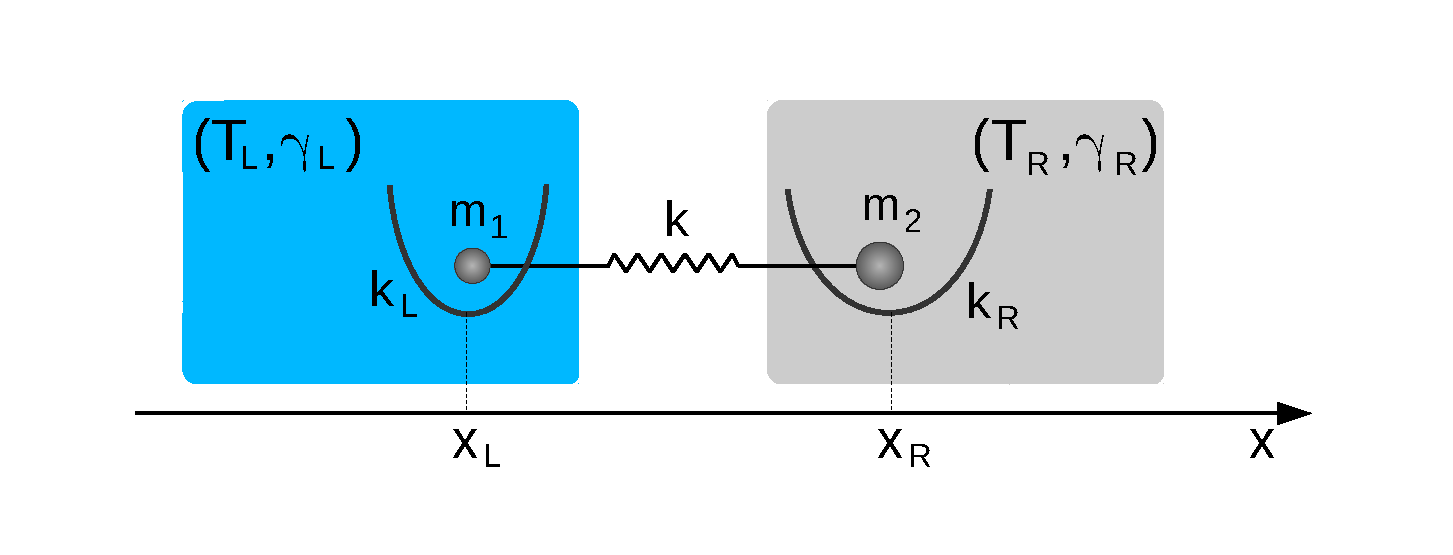
\includegraphics[width=1.1\linewidth]{Figures/model_diagram.pdf}
  \caption{Diagram of the model described in Section \ref{sec:Physical_Model}. Two ions coupled to each other through a spring constant $k$. Each ion is harmonically trapped and connected to a bath characterized by its temperature $T_i$ and its friction coefficient $\gamma_i$. }
  \label{fig:model_diagram}
\end{figure}

\section{Physical Model \label{sec:Physical_Model}}

The physical model consists of two masses $m_1$ and $m_2$ coupled to each other by a harmonic interaction with spring constant $k$ and natural length $x_e$. Each of the masses $m_1$ and $m_2$ are confined by a harmonic potential with spring constants $k_L$, $k_R$ and equilibrium positions $x_L$, $x_R$ respectively (see Fig. \ref{fig:model_diagram}). The Hamiltonian describing this model is
%
\begin{equation}
  H = \frac{p_1^2}{2m_1} + \frac{p_2^2}{2m_2} + V(x_1,x_2),
  \label{eq:HamiltonianOriginalCordinates}
\end{equation}
%
with $V(x_1,x_2)=\frac{k}{2}\left( x_1 - x_2 - x_e \right)^2 + \frac{k_L}{2}\left( x_1 - x_L \right)^2 + \frac{k_R}{2}\left( x_2 - x_R \right)^2$,  where $\{x_i,p_i\}_{i=1,2}$ are the position and momentum of each mass. Switching from the original coordinates $x_i$ to displacements with respect to the equilibrium positions of the system $q_i = x_i - x_i^{eq}$, where $x_i^{eq}$ are the solutions to $\partial_{x_i}V(x_1,x_2)=0$, the Hamiltonian can be written as
%
\begin{align}
  H &= \frac{p_1^2}{2m_1} + \frac{p_2^2}{2m_2} + \frac{k+k_L}{2}q_1^2\nonumber\\ &+ \frac{k+k_R}{2}q_2^2 - k q_1 q_2 + V(x_1^{eq},x_2^{eq}).
  \label{eq:Hamiltonian}
\end{align}
%
This has the form of  the Hamiltonian of a system around a stable equilibrium point
%
\begin{equation}
  H = \frac{1}{2} \overrightarrow{p}^\mathsf{T}\mathbb{M}^{-1}\overrightarrow{p} + \frac{1}{2} \overrightarrow{q}^\mathsf{T}\mathbb{K}\overrightarrow{q},
\label{generic}
\end{equation}
%
where $\overrightarrow{q} = \left(q_1,q_2\right)^\mathsf{T}$, $\overrightarrow{p} = \left(p_1,p_2\right)^\mathsf{T}$, $\mathbb{M} = diag(m_1,m_2)$ is the mass matrix of the system and $\mathbb{K}$ is the Hessian matrix of the potential at the equilibrium point, i.e., $\mathbb{K}_{ij} = \partial^2_{x_i,x_j}V(\overrightarrow{x})\Big|_{\overrightarrow{x} = \overrightarrow{x}^{eq}}$. In this model  $\mathbb{K}_{11} = k + k_L$, $\mathbb{K}_{22} = k + k_R$ and $\mathbb{K}_{12} = \mathbb{K}_{21} = -k$.
We shall see later that
the generic form (\ref{generic}) can be adapted to different physical settings, in particular to
two ions in individual traps, or to two ions in a common trap.

The  masses are in contact with Langevin baths, which will be denoted as $L$ (for left) and $R$ (for right), at temperatures $T_{L}$ and $T_R$ for  the mass $m_1$ and $m_2$ respectively (see Fig. \ref{fig:model_diagram}). The equations of motion of the system, taking into account the Hamiltonian and the Langevin baths are
%
\begin{align}
  \dot{q}_1 &= \frac{p_1}{m_1},\nonumber
  \\
  \dot{q}_2 &= \frac{p_2}{m_2},\nonumber
  \\
  \dot{p}_1 &= -(k+k_L)q_1 + k q_2 -\frac{\gamma_L}{m_1} p_1 + \xi_L(t),\nonumber
  \\
  \dot{p}_2 &= -(k+k_R)q_2 + k q_1 -\frac{\gamma_R}{m_2} p_2 + \xi_R(t),
\end{align}
%
where $\gamma_L$, $\gamma_R$ are the friction coefficients of the baths and $\xi_L(t)$, $\xi_R(t)$ are Gaussian white-noise-like forces. The Gaussian forces have zero mean ($\expval{ \xi_L(t) } = \expval{ \xi_R(t) } = 0 $) and satisfy the correlations $\expval{ \xi_L(t)\xi_R(t') } = 0$, $\expval{ \xi_L(t)\xi_L(t') } = 2D_L\delta(t-t')$, $\expval{ \xi_R(t)\xi_R(t') } = 2D_R\delta(t-t')$. $D_L$ and $D_R$ are the diffusion coefficients, which satisfy the fluctuation-dissipation theorem: $D_L = \gamma_L k_B T_L$, $D_R =\gamma_R k_B T_R$ ($k_B$ is the Boltzmann constant).

It is useful to define the phase-space vector $\overrightarrow{r}(t) = \left( \overrightarrow{q}, \mathbb{M}^{-1}\overrightarrow{p} \right)^\mathsf{T}$ (note that $\overrightarrow{v} = \mathbb{M}^{-1}\overrightarrow{p}$ is just the velocity vector) so the equations of motion for this vector are
%
\begin{equation}
  \dot{\overrightarrow{r}}(t) = \mathbb{A} \, \overrightarrow{r}(t) + \mathbb{L}\overrightarrow{\xi}(t),
  \label{eq:vectorEqOfMotion}
\end{equation}
%
with
%
\begin{align}
  \mathbb{A} &=
  \left(
  \begin{array}{cc}
    \mathbb{0}_{2 \times 2} & \mathbb{1}_{2 \times 2}
    \\
    -\mathbb{M}^{-1}\mathbb{K} & -\mathbb{M}^{-1}\Gamma
  \end{array}
  \right),
  \nonumber
  \\
  \mathbb{L} &=
  \left(
  \begin{array}{c}
    \mathbb{0}_{2\times 2} \\ \mathbb{M}^{-1}
  \end{array}
  \right),
\end{align}
%
and $\overrightarrow{\xi}(t) = \left( \xi_L(t),\xi_R(t) \right)^\mathsf{T}$, $\Gamma = diag(\gamma_L,\gamma_R)$. $\mathbb{0}_{n\times n}$ and $\mathbb{1}_{n\times n}$ are the $n$-th dimensional squared 0 matrix and identity matrix respectively. With the vector notation the correlation of the white-noise forces can be written as
%
\begin{equation}
  \expval{\overrightarrow{\xi}(t)\overrightarrow{\xi}(t')^\mathsf{T}} = 2 \mathbb{D}\delta(t-t'),
\end{equation}
%
with $\mathbb{D} = diag(D_L,D_R)$.
%
%
%
%
%
%
\section{Covariance matrix in the steady state\label{sec:covMatrix}}
%
%
%
%
%
%
We define the covariance matrix of the system as $\mathbb{C}(t) = \expval{\overrightarrow{r}(t)\overrightarrow{r}(t)^\mathsf{T}}$. This matrix is important because the heat transport properties can be extracted from it. In particular, the kinetic temperatures of the masses, $T_1(t)$ and  $T_2(t)$, are
%
\begin{align}
  T_1(t) &= \frac{\expval{ p_1^2(t)}}{m_1 k_B} = \frac{m_1 C_{3,3}(t)}{k_B},
  \nonumber\\
   T_2(t) &= \frac{\expval{ p_2^2(t)}}{m_2 k_B} = \frac{m_2 C_{4,4}(t)}{k_B}.
  \label{eq:Temperature_definition}
\end{align}
%
One approach to find the covariance matrix is to solve Eq. \eqref{eq:vectorEqOfMotion}. However, this requires solving the equations explicitly or simulate them numerically many times to find the covariance matrix for the ensemble of simulated stochastic trajectories. Instead, we proceed by looking for an ordinary differential equation that gives the evolution of the covariance matrix as described in \cite{Sarkka2019,Rieder1967,Casher1971}. Differentiating $\mathbb{C}(t)$ with respect to time and using Eq. \eqref{eq:vectorEqOfMotion} we get
%
\begin{align}
  \frac{d}{dt}\mathbb{C}(t) &=
  \mathbb{A}\mathbb{C}(t) +
  \mathbb{C}(t) \mathbb{A}^\mathsf{T}
  \nonumber\\
  &+
  \mathbb{L}\expval{ \overrightarrow{\xi}(t)\overrightarrow{r}(t)^\mathsf{T}}
  \nonumber\\
  &+
  \expval{ \overrightarrow{r}(t)\overrightarrow{\xi}(t)^\mathsf{T}}\mathbb{L}^\mathsf{T}.
  \label{eq:evolutionOfCovariances}
\end{align}
%
The solution of Eq. \eqref{eq:evolutionOfCovariances} allows us to find the local temperatures of the masses as a function of the bath temperatures (Eq. \eqref{eq:Temperature_definition}) at all times. In particular, we are interested in the covariance matrix in the steady state, i.e., for $t\to \infty$. According to the Novikov Theorem \cite{Novikov1965} we can write down the covariance matrix in the steady state without having to integrate the differential equation. We now show how to get the steady-state covariance matrix.

In the steady state, the covariance matrix is constant ($\frac{d}{dt}\mathbb{C}(t)=0$), therefore it satisfies
%
\begin{align}
  &\mathbb{A}\mathbb{C}^{s.s.} +
  \mathbb{C}^{s.s.} \mathbb{A}^\mathsf{T}=
  \nonumber\\
  &- \mathbb{L}\expval{ \overrightarrow{\xi}\overrightarrow{r}^\mathsf{T}}^{s.s.}
  - \expval{ \overrightarrow{r}\overrightarrow{\xi}^\mathsf{T}}^{s.s.}\mathbb{L}^\mathsf{T},
  \label{eq:SteadyStateEquation_raw}
\end{align}
%
with $\{\cdot\}^{s.s.}\equiv \lim\limits_{t \to \infty} \{\cdot\}(t)$. Equation \eqref{eq:SteadyStateEquation_raw} is an algebraic equation whose solution is the steady-state covariance matrix $\mathbb{C}^{s.s.}$. However, the two terms $\expval{ \overrightarrow{\xi}\overrightarrow{r}^\mathsf{T}}^{s.s.}$ and  $\expval{\overrightarrow{r}\overrightarrow{\xi}^\mathsf{T}}^{s.s.}$ need to be calculated before working out the solution. One approach to calculate $\expval{\overrightarrow{\xi}\overrightarrow{r}^\mathsf{T}}^{s.s.}$ would be to solve Eq. \eqref{eq:vectorEqOfMotion}, but this is exactly what we are trying to avoid. It is here when the Novikov theorem comes useful, since it lets us compute $\expval{ \overrightarrow{\xi}\overrightarrow{r}^\mathsf{T}}^{s.s.}$ without having to integrate the equations of motion. Using this theorem and the $\delta$-correlation of the noises, we find the $ij$-th component of $\expval{ \overrightarrow{\xi}(t)\overrightarrow{r}(t)^\mathsf{T}}$,
%
\begin{align}
  \expval{ \xi_i(t) r_j(t) } &= \sum_{k=1}^2 \int_0^t d\tau\,\expval{ \xi_i(t) \xi_k(\tau)}
  \,
  \expval{ \frac{\delta r_j(t)}{\delta \xi_k(\tau)} }\nonumber
  \\
  &= \sum_{k=1}^2 \mathbb{D}_{ik}
  \,
  \lim_{\tau \to t^{-}}
  \,
  \expval{ \frac{\delta r_j(t)}{\delta \xi_k(\tau)} },
\end{align}
%
where $\lim\limits_{\tau \to t^{-}}$ is the limit when $\tau$ goes to $t$ from below. Evaluation of the functional derivative ${\delta r_j(t)}/{\delta \xi_k(\tau)}$ for the $\tau \to t^{-}$ limit gives
%
\begin{equation}
  \expval{ \overrightarrow{\xi}(t)\overrightarrow{r}(t)^\mathsf{T}} = \mathbb{D}\mathbb{L}^\mathsf{T}.
\end{equation}
%
Now, the algebraic equation that gives the steady-state covariance matrix becomes
%
\begin{equation}
  \mathbb{A}\mathbb{C}^{s.s.} +
  \mathbb{C}^{s.s.}\mathbb{A}^\mathsf{T}
  =
  -\mathbb{B},
  \label{eq:SteadyStateEquationToyModel}
\end{equation}
%
with $\mathbb{B} = 2 \mathbb{L}\mathbb{D}\mathbb{L}^\mathsf{T}$. By definition, the covariance matrix is  symmetric, but there are also  additional restrictions imposed by the equations of motion and the steady-state condition, which reduce the dimensionality of the problem of solving Eq. \eqref{eq:SteadyStateEquationToyModel} \cite{Simon2019}. Since ${d \expval{ q_i q_j }}/{dt} = 0$ in the steady state, we have
%
\begin{align}
  \expval{ p_1 q_1}^{s.s.} &= \expval{ p_2 q_2}^{s.s.} = 0,\nonumber\\
  \frac{\expval{ p_1 q_2}^{s.s.}}{m_1}&=-\frac{\expval{ q_1 p_2}^{s.s.}}{m_2}.
  \label{eq:ExtraConditionSteadyState}
\end{align}
%
Taking \eqref{eq:ExtraConditionSteadyState} into account, the steady-state covariance matrix takes the form
%
\begin{equation}
  \begin{split}
    \mathbb{C}^{s.s.} =
    \left(
    \begin{array}{cccc}
      \expval{ q_1^2}^{s.s.}  & \expval{ q_1 q_2}^{s.s.}  & 0 & \frac{\expval{ p_2 q_1}^{s.s.} }{m_2} \\
      \expval{ q_1 q_2}^{s.s.}  & \expval{ q_2^2}^{s.s.}  & -\frac{\expval{ p_2 q_1}^{s.s.} }{m_2} & 0 \\
      0 & -\frac{\expval{ p_2 q_1}^{s.s.} }{m_2} & \frac{\expval{ p_1^2}^{s.s.} }{m_1^2} & \frac{\expval{ p_1 p_2}^{s.s.} }{m_1 m_2} \\
      \frac{\expval{ p_2 q_1}^{s.s.} }{m_2} & 0 & \frac{\expval{ p_1 p_2}^{s.s.} }{m_1 m_2} & \frac{\expval{ p_2^2}^{s.s.} }{m_2^2} \\
      \end{array}
      \right)
    \end{split}
    \label{eq:steadyStateCovarianceMatrix}\,.
\end{equation}
%
The explicit set of equations for the components of $\mathbb{C}^{s.s}$ can be found in Appendix \ref{Appendix:SteadyStateEquations}.
%
%
%
%
%
\section{Solutions\label{sec:solutions}}
%
%
%
%

%
In this section we use the solution to Eq. \eqref{eq:SteadyStateEquationToyModel} to write down the temperatures and currents in the steady state. We use Mathematica to obtain analytic expressions for the temperatures,
%
\begin{align}
  T_1 &= \frac{T_L \mathcal{P}_{1,L}(k) + T_R \mathcal{P}_{1,R}(k)}{\mathcal{D}(k)},\nonumber
  %
  \\
  %
  T_2 &= \frac{T_L \mathcal{P}_{2,L}(k) + T_R \mathcal{P}_{2,R}(k)}{\mathcal{D}(k)},
  %
  \label{eq:ModelBTemperatures}
\end{align}
%
where $\mathcal{D}(k) =  \sum\limits_{n=0}^2 \mathcal{D}_n k^n$ and $\mathcal{P}_{i,(L/R)}(k) = \sum\limits_{n=0}^2 a_{i,n,(L/R)} k^n$ are polynomials in the coupling constant $k$ with coefficients
%
\begin{align}
  \mathcal{D}_0 &= a_{1,0,L} = a_{2,0,R} = \gamma _L \gamma _R \left[h^{(1)} \left(\gamma_L k_R +\gamma_R k_L \right)+\left(m_1 k_R-m_2 k_L\right)^2\right],\nonumber
  %
  \\
  %
  \mathcal{D}_1 &= a_{1,1,L} = a_{2,1,R} = \gamma _L \gamma _R \left[h^{(0)} h^{(1)}+2 \left(m_1-m_2\right) \left(m_1 k_R-m_2 k_L\right)\right],\nonumber
  %
  \\
  %
  \mathcal{D}_2 &= h^{(0)} h^{(2)},\nonumber
  %
  \\
  %
  a_{1,2,L} &= \gamma _L \left(m_2 h^{(1)} + \gamma_R (m_1 - m_2)^2 \right),\nonumber
  %
  \\
  %
  a_{1,2,R} &= h^{(1)} m_1 \gamma_R,\nonumber
  %
  \\
  %
  a_{2,2,L} &= h^{(1)} m_2 \gamma_L,\nonumber
  %
  \\
  %
  a_{2,2,R} &= \gamma _R \left( m_1 h^{(1)} + \gamma_L (m_1-m_2)^2 \right),\nonumber
  %
  \\
  %
  a_{1,0,R} &= a_{1,1,R} = a_{2,0,L} = a_{2,1,L} = 0,
  %
  \label{eq:SolutionPolynomialCoefficients}
\end{align}
%
where $h^{(n)}\equiv \gamma_R m_1^n + \gamma_L m_2^n$. The currents from the baths to the masses \cite{Simon2019} are
%
\begin{equation}
  \begin{split}
    J_L &= k_B \frac{\gamma_L}{m_1} \left( T_L - T_1 \right),\\
    J_R &= k_B \frac{\gamma_R}{m_2} \left( T_R - T_2 \right),
    \label{eq:currents_definition}
  \end{split}
\end{equation}
\\
%
with $T_i$ given by Eq. \eqref{eq:ModelBTemperatures}. Since, in the steady state, $J_L = -J_R$ we will use the shorthand notation $J \equiv J_L$. Substituting Eq. \eqref{eq:ModelBTemperatures} into Eq.  \eqref{eq:currents_definition} we get for the heat current
%
% \begin{equation}
%   J = k_B \frac{k^2\gamma_L \gamma_R h^{(1)}}{\mathcal{D}(k)}(T_L - T_R).
%   \label{eq:CurrentsInModelB}
% \end{equation}
%
\begin{equation}
  J = \kappa\;(T_L - T_R),
  \label{eq:CurrentsInModelB}
\end{equation}
%
where $\kappa = k_B {k^2\gamma_L \gamma_R h^{(1)}}/{\mathcal{D}(k)}$ acts as an effective thermal conductance, which depends on the parameters of the system, i.e., the masses and spring constants, and also on the friction coefficients of the baths. From Eq. \eqref{eq:CurrentsInModelB} it could be thought that inverting the temperatures of the baths would only lead to an exchange of heat currents. However, since the thermal conductance $\kappa$ depends on the friction coefficients, the exchange of the baths implies a change in its value. Moreover, it is possible to have temperature-dependent friction coefficients, as it happens in the physical set-up of laser-cooled trapped ions described in Section \ref{sec:TrappedIonSetUp}.
%
%


\section{Relation of the Model to a trapped ion set-up \label{sec:TrappedIonSetUp}}

As we mentioned, the parameters $k$, $k_L$ and $k_R$ can be related to the elements of the Hessian matrix of a system in a stable equilibrium position. In this section we will identify these parameters with the Hessian matrix of a pair of trapped ions. Here we consider two different set-ups: two ions in a collective trap, and two ions in individual traps. In Section \ref{sec:lookingForR} we focus on two ions in individual traps to illustrate the analysis of rectification.

In both set-ups we assume strong confinement in the radial direction, making the effective dynamics one-dimensional. We will also assume that the confinement in the axial direction is purely electrostatic, which makes the effective spring constant independent of the mass of the ions \cite{Leibfried2003}. Additionally, we will relate the temperatures and friction coefficients of the Langevin baths to those corresponding to Doppler cooling.

\subsection{Collective trap}

Consider two ions of unit charge with masses $m_1$ and $m_2$ trapped in a collective trap. Assuming strong radial confinement and purely electrostatic axial confinement, both ions feel the same harmonic oscillator potential with trapping constant $k_{trap}$ \cite{Leibfried2003}. The potential describing the system is
%
\begin{equation}
  V_{collective} = \frac{1}{2}k_{trap} \left( x_1^2 + x_2^2\right) + \frac{\mathcal{C}}{x_2-x_1},
\end{equation}
%
with $\mathcal{C}=\frac{Q^2}{4\pi\varepsilon_0}$. The equilibrium positions for this potential are
%
\begin{equation}
  x_2^{eq} = -x_1^{eq} =
  \label{eq:equilibriumPositionsCollectiveTrap}\left(\frac{1}{2}\right)^{2/3} \left(\frac{Q^2}{4\pi\varepsilon_0 k_{trap}}\right)^{1/3}.
\end{equation}
%
Assuming small oscillations of the ions around the equilibrium positions, the Hessian matrix of the system is
%
\begin{align}
  \mathbb{K}_{1,2} &= -\frac{Q^2}{2\pi\varepsilon_0}\frac{1}{(x_2^{eq}-x_1^{eq})^3} = -k_{trap},\nonumber
  \\
  \mathbb{K}_{1,1} &= k_{trap} + \frac{Q^2}{2\pi\varepsilon_0}\frac{1}{(x_2^{eq}-x_1^{eq})^3} = 2 k_{trap},\nonumber
  \\
  \mathbb{K}_{2,2} &= k_{trap} + \frac{Q^2}{2\pi\varepsilon_0}\frac{1}{(x_2^{eq}-x_1^{eq})^3} = 2 k_{trap}.
  \label{eq:HessianOffDiagonalCollective}
\end{align}
%
Using Eq. \eqref{eq:HessianOffDiagonalCollective} we can relate the parameters of this physical set-up to those of the model described in Section \ref{sec:Physical_Model} to find
%
\begin{equation}
  k_L = k_R = k = k_{trap}.
\end{equation}
%

\subsection{Individual on-site traps}

We can make the same assumptions for the axial confinement as in the previous subsection but now each of the ions is in an individual trap with spring constants $k_{trap,L}$ and $k_{trap,R}$ respectively. The potential of the system is
%
\begin{align}
    V_{individual} &= \frac{1}{2}k_{trap,L}\left(x_1 -x_L\right)^2 +\frac{1}{2}k_{trap, R}\left(x_2 -x_R\right)^2 \nonumber \\&+ \frac{\mathcal{C}}{x_2-x_1},
\end{align}
%
where $x_L$ and $x_R$ are the center positions of the on-site traps. The elements of the Hessian matrix in the equilibrium position are
%
\begin{align}
  \mathbb{K}_{1,2} &= -\frac{Q^2}{2\pi\varepsilon_0}\frac{1}{(x_2^{eq}-x_1^{eq})^3},\nonumber
  \\
  \mathbb{K}_{1,1} &= k_{trap,L} + \frac{Q^2}{2\pi\varepsilon_0}\frac{1}{(x_2^{eq}-x_1^{eq})^3},\nonumber
  \\
  \mathbb{K}_{2,2} &= k_{trap,R} + \frac{Q^2}{2\pi\varepsilon_0}\frac{1}{(x_2^{eq}-x_1^{eq})^3}.
  \label{eq:HessianOffDiagonalOnSite}
\end{align}
%
Comparing the parameters in Eq. \eqref{eq:HessianOffDiagonalOnSite} with those in the model described in Section \ref{sec:Physical_Model} we identify
\begin{align}
  k_L &= k_{trap,L},\nonumber\\
  k_R &= k_{trap,R},\nonumber\\
  k &= \frac{Q^2}{2\pi\varepsilon_0}\frac{1}{(x_2^{eq}-x_1^{eq})^3}\,.
\end{align}
%
In this case, the analytic expressions for the equilibrium positions are more complicated. We get for the distance between the equilibrium positions of the ions
%
\begin{align}
  &(x_2 - x_1)^{(eq)} = \frac{1}{3} \Delta x_{LR}\nonumber\\
  &- \frac{1}{6}\Big[ \frac{2^{2/3}\zeta}{k_{trap,L} k_{trap,R} (k_{trap,L} + k_{trap,R})}\nonumber\\
  &+ \frac{2^{4/3} k_{trap,L} k_{trap,R} (k_{trap,L} + k_{trap,R}) (x_R-x_L)^2}{\zeta} \Big]\,,
\end{align}
%
where $\Delta x_{LR} = (x_R-x_L)$ and $\zeta = \left( Y - \eta \right)^{(1/3)}$, with
%
\begin{align}
  &Y = 3 \sqrt{3} \bigg\{\mathcal{C} k_{trap,L}^4 k_{trap,R}^4 \left(k_{trap,L}+k_{trap,R}\right)^{7}\times\nonumber\\& \quad\quad \left[4 k_{trap,L} k_{trap,R} \Delta x_{LR}^3+27 \mathcal{C} \left(k_{trap,L}+k_{trap,R}\right)\right]\bigg\}^{(1/2)},\nonumber
  %
  \\
  %%
  &\eta =  k_{trap,L}^2 k_{trap,R}^2 \left(k_{trap,L}+k_{trap,R}\right)^{3}\times\nonumber\\ &\quad\quad\left[2 k_{trap,L} k_{trap,R} \Delta x_{LR}^3+27 \mathcal{C} \left(k_{trap,L}+k_{trap,R}\right)\right]\,.
\end{align}
%
In this set-up, the coupling between the ions $k$ can be controlled by changing the distance between the on-site traps.



\subsection{Optical molasses and Langevin baths}

Trapped ions may be cooled down by a pair of counterpropagating lasers which are red-detuned with respect to an internal atomic transition of the ions. This technique is known as Doppler cooling or optical molasses \cite{Chu1985,Cohen1992,Metcalf1999,Metcalf2003}. The off-resonant absorption of laser photons by the ions exerts a damping-like force that slows them down. The spontaneous emission of the ions produces heating due to the random recoil generated by the emitted photons. Both, the friction and recoil force are in balance, and eventually the ion thermalizes to a finite temperature.
Thus the effect of the lasers on the ion is equivalent to a Langevin bath with temperature $T_{molass}$ and friction coefficient $\gamma_{molass}$. The temperature and friction coefficients are controlled with the laser intensity $I$ and frequency detuning $\delta$ with respect to the selected internal transition by the expressions \cite{Cohen1992,Metcalf2003,Ruiz2014},
%
\begin{align}
  \gamma_{molass}(I,\delta) &= -4 \hbar \left(\frac{\delta + \omega_0}{c}\right)^2 \left(\frac{I}{I_0}\right)\frac{2\delta/\Gamma}{\left[1 + (2\delta/\Gamma)^2\right]^2},\nonumber\\
  %
  T_{molass}(\delta) &= -\frac{\hbar \Gamma}{4 k_B} \frac{1+(2\delta/\Gamma)^2}{(2\delta/\Gamma)},
  \label{eq:DopplerCoolingToyModel}
\end{align}
%
where $\omega_0$ is the frequency of the selected internal atomic transition, $\Gamma$ is the natural width of the excited state, and $I_0$ is the saturation intensity.
%
%
%
\section{Looking for rectification\label{sec:lookingForR}}
%
%
%
%First let us define what we exactly mean by \textit{rectification}.
We will say that we observe rectification whenever the heat current $J$ for a configuration of the baths changes when we exchange the baths to $\tilde{J}$. The important point here is to define what is  meant by \textit{exchanging the baths}. We consider that a bath is characterized, not only by its temperature $T$ but also by its coupling  to the system by means of the friction coefficient $\gamma$, so, exchanging the baths is achieved by exchanging both the temperatures and the friction coefficients, as summarized in Table \ref{tab:reversed_bath}.

When implementing temperatures and friction coefficients by lasers, this exchange operation is performed by changing the values of the intensities and detunings acting on each ion (Eq. \eqref{eq:DopplerCoolingToyModel}). The exchange operation is straightforward when the two ions are either of the same species or isotopes of each other, since the only required action is to exchange the values of the detunings of the lasers without modifying the intensities. However, if we deal with two different species, i.e., with two different atomic transitions, the laser wavelengths and the decay rates  depend on the species. Then, exchanging the temperatures by modifying the detunings, keeping the laser intensities constant, does not necessarily imply an exchange of the friction coefficients. Nevertheless it is possible to adjust the laser intensities so that the friction coefficients get exchanged and that is the assumption hereafter. The idea of implementing a bath exchange like this follows the same line of thought as \cite{Pereira2017}, since we are adding a temperature dependent feature to the system -the friction coefficients- that changes as the baths are inverted.

\begin{figure}
  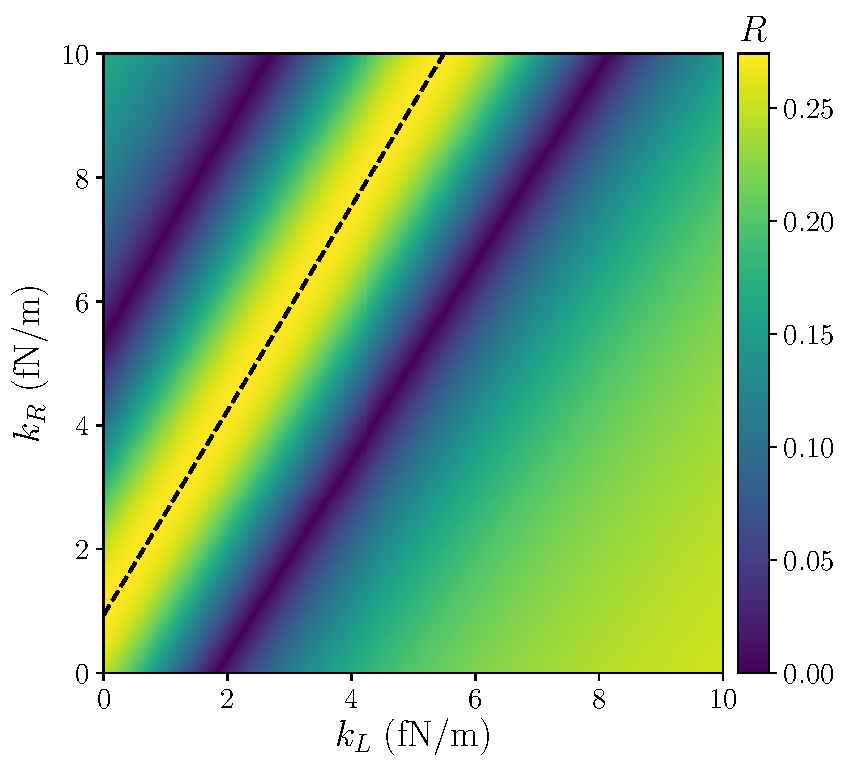
\includegraphics[width=\linewidth]{Figures/RwMPlota.pdf}
  \caption{Rectification, $R$, in the $k_L k_R$ plane for $k = 1.17 \times$ fN/m, $\gamma_L = 6.75\times 10^{-22}$ kg/s, and $\gamma_R = 4.64\gamma_L$.}
  \label{fig:Fig_rectification_K_plane}
\end{figure}

To measure rectification, we will use the rectification coefficient $R$ defined as
%
\begin{equation}
  R = \frac{\abs{J-\tilde{J}}}{\max(J,\tilde{J})},
  \label{eq:Rectification}
\end{equation}
%
that is, the ratio between the difference of heat currents and the largest one. As defined, $R=0$ for no asymmetry of the heat currents and $R=1$ when they are maximally asymmetric.

\begin{table}[]
\caption{Definition of forward and reversed (exchanged) bath configurations.}
\begin{tabular}{lcc}
\hline
                 & forward                & reversed                                                       \\ \hline
Bath Friction    & $\gamma_L$, $\gamma_R$ & $\tilde{\gamma}_L =\gamma_R $,  $\tilde{\gamma}_R =\gamma_L $   \\
Bath Temperature & $T_L$, $T_R$           & $\tilde{T}_L =T_R $,  $\tilde{T}_R =T_L $                     \\
\hline
\end{tabular}
\label{tab:reversed_bath}
\end{table}

\subsection{Parametric exploration}

We have explored thoroughly the space formed by the parameters of the model to find asymmetric heat transport, namely, $m_1,m_2,k,k_L,k_R,\gamma_L,\gamma_R$. We have fixed the values of some of the parameters to realistic ones while we have varied the rest. We have set the masses to $m_1 = 24.305$ a.u. and $m_2 = 40.078$ a.u., which correspond to Mg and Ca, whose ions are broadly used in trapped-ion physics. The temperatures are also fixed and, as Eq. \eqref{eq:CurrentsInModelB} shows, rectification does not formally depend on the temperature in this model, unless we set the friction coefficients as a function of temperature using Eq. \eqref{eq:DopplerCoolingToyModel} explicitly.

Figure \ref{fig:Fig_rectification_K_plane} depicts the values of the rectification after sweeping the $k_L k_R$ plane for fixed values of $k$, $\gamma_L$, and $\gamma_R$. A remarkable result from this figure is that parallel lines appear alternating minima and maxima of $R$. With a numerical fitting, we find that the line corresponding to the highest maximum value of $R$ is determined by
%
\begin{equation}
  \frac{k+k_L}{m_1} = \frac{k+k_R}{m_2}.
  \label{eq:MaxRLines}
\end{equation}
%
In a trapped-ion context the condition \eqref{eq:MaxRLines} may be imposed by adjusting the distance of the traps for fixed $k_L$ and $k_R$. It is also  remarkable that when Eq. \eqref{eq:MaxRLines} is satisfied, the rectification no longer depends on the spring constants of the model. This last result can be  found assuming  Eq. \eqref{eq:MaxRLines} when calculating the currents with Eq. \eqref{eq:CurrentsInModelB} and $R$ with Eq. \eqref{eq:Rectification},
%
\begin{equation}
    R=
    \begin{cases}
      1-\frac{a+g}{1+ag} &\text{ if }(a+g)<(1+ag)\\
      1-\frac{1+ag}{a+g} &\text{ if }(a+g)>(1+ag)\\
      0 &\text{ if } (a+g)=(1+ag)\,,
    \end{cases}
  \label{eq:maxRExpression}
\end{equation}
%
where $a$ and $g$ are the mass and friction coefficients ratios
%
\begin{align}
  a &= m_2/m_1,\nonumber\\
  g &= \gamma_R/\gamma_L.
\end{align}
%
The maximal rectification found does not scale with the magnitude of the masses or the friction coefficients, just with their ratios. Besides a high $R$, it is important to have non-vanishing heat currents
%, as in some cases an increase of $R$ is accompanied by an overall decrease of the heat currents
\cite{Simon2019}. Using again  Eq. \eqref{eq:MaxRLines} in the expression for the currents \eqref{eq:CurrentsInModelB}, the maximum current $J_{\max} = \max(\big|{J}\big|,\big|\tilde{J}\big|)$ is
%
\begin{align}
    &J_{\max}=\begin{cases}
   \frac{k_B g\gamma_L k^2 \abs{T_L-T_R}}{(a+g)(g\gamma_L^2(k_L+k)+k^2m_1)} & \text{ if }(a+g)<(1+ag)
    \\
    \frac{k_B g\gamma_L k^2 \abs{T_L-T_R}}{(1+ag)(g\gamma_L^2(k_L+k)+k^2m_1)}& \text{ if }(a+g)>(1+ag)\,.
    \end{cases}
    \label{eq:maxJExpression}
\end{align}
%
Now we analyze how the parameters $a$ and $g$ affect the maximum current $J_{max}$ in \eqref{eq:maxJExpression}. To do this, we can divide the $ag$ plane in four quadrants by the axes $a = 1$ and $g = 1$ (in those axes $R = 0$). In Eq. \eqref{eq:maxJExpression} the parameter $a$ appears only in the denominator, thus for a higher $a$, a smaller current is found. The quadrants with $a < 1$ will be better for achieving large currents. However, $g$ appears both in the numerator and denominator so there is no obvious advantageous quadrant for this parameter.

Equation \eqref{eq:maxRExpression} is symmetric upon the transformations $a \leftrightarrow 1/a$ and $g \leftrightarrow 1/g$. Using a logarithmic scale for $a$ and $g$, the resulting $R$ map will be symmetric with respect to the $a=1$ and $g=1$ axes. We can limit ourselves to analyze the quadrant $a > 1$, $g > 1$, as the results in other quadrants will be equivalent upon transformations $a \leftrightarrow 1/a$ and $g \leftrightarrow 1/g$.


\begin{figure}
  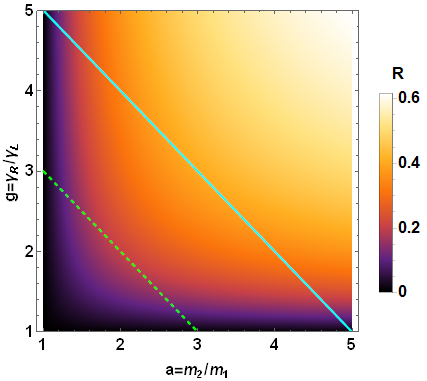
\includegraphics[width=\linewidth]{Figures/Rade.png}
  \caption{Rectification factor, $R$, given by Eq. \eqref{eq:maxRExpression}.}
  \label{fig:R_g_a_plane}
\end{figure}

Fig. \ref{fig:R_g_a_plane} shows the rectification given by Eq. \eqref{eq:maxRExpression} in terms of $a$ and $g$. Along any diagonal line (parallel to the solid cyan or the dashed green lines), the maximum value is at the center, that is, when $a = g$. However, if we fix $a$, increasing $g$ always increases $R$. Although we could increase $g$ arbitrarily to get more rectification this is not a realistic option in a trapped-ion set-up. Since $g$ is defined as the ratio between the friction coefficients, increasing it means making either $\gamma_L$ go to 0 or $\gamma_R$ to infinity. Making $\gamma_L$ go to 0 decouples one of the ions from the bath, so the heat current tends to vanish in any direction. Also, increasing $\gamma_R$ arbitrarily is impossible since the Doppler cooling friction coefficient as a function of the laser detuning (Eq. \eqref{eq:DopplerCoolingToyModel}) is bounded. Although Eq. \eqref{eq:DopplerCoolingToyModel} suggests that boosting the laser intensity can also increase the friction coefficient, this is not an option since Eq. \eqref{eq:DopplerCoolingToyModel} is just an approximation for low laser intensities. When going to higher intensities, the emission/absorption of photons by the ion is saturated and the friction coefficient reaches a finite value proportional to the width $\Gamma$ of the excited state \cite{Metcalf2003}. As a compromise between feasibility and high $R$, we set the ratio between the friction coefficients $g$ to be equal to the mass ratio $a$. As shown  in Fig. \ref{fig:R_g_a_plane}, along the solid-cyan and dashed-green diagonal lines the maximum $R$ is achieved for $a = g$. Fig. \ref{fig:Fig_PerfectRectification} shows the rectification in Eq. \eqref{eq:maxRExpression} for the line $a = g$. When both parameters are large enough, the rectification goes to 1.
%
%
\subsection{Spectral match/mismatch approach to rectification}
%
%
%
\begin{figure}
  \includegraphics[width=\linewidth]{Figures/CC-eps-converted-to.pdf}
  \caption{Rectification for different values of $c=m_2/m_1=\gamma_R/\gamma_L$ when the maximum condition in the $k_L k_R$ plane is satisfied (Eq. \eqref{eq:MaxRLines}).}
  \label{fig:Fig_PerfectRectification}
\end{figure}

The match/mismatch between the power spectra of the particles controls the heat currents in the system \cite{Terraneo2002,Li2004}. A good match between the power spectra of the two ions in a large range of frequencies yields a higher heat current through the system while the mismatch  reduces the heat current.
%Therefore, we can understand rectification through the match/mismatch of the phonon bands of the ions \cite{Terraneo2002}.
If there is a good match between the spectra of the ions (i.e., their peaks overlap in a broad range of frequencies) for a certain baths configuration, and mismatch when the baths exchange, the system will present heat rectification.

We have studied the phonon spectra of our model for several sets of parameters exhibiting no rectification or strong rectification. The phonon spectra of the ions is calculated through the spectral density matrix. For a real-valued stochastic process $\overrightarrow{x}(t)$, its spectral density matrix is defined as \cite{Sarkka2019}
%
\begin{equation}
  \mathbb{S}_{\overrightarrow{x}}(\omega) \equiv \expval{ \overrightarrow{X}(\omega) \overrightarrow{X}^\mathsf{T}(-\omega) },
  \label{eq:SpectralDensityDefinition}
\end{equation}
%
with $\overrightarrow{X}(\omega)$ being the Fourier transform of $\overrightarrow{x}(t)$ (we are using the convention of multiplying by a factor of $1$ and $\frac{1}{2\pi}$ for the transform and its inverse operation). A justification of the use of the spectral density matrix to understand heat transport arises from the Wiener-Khinchin theorem \cite{Sarkka2019}, which says that the correlation matrix of a stationary stochastic process in the steady state is the inverse Fourier transform of its spectral density matrix $\expval{\overrightarrow{r}(t)\overrightarrow{r}^\mathsf{T}(t+\tau)} = \mathcal{F}^{-1}[\mathbb{S}_{\overrightarrow{r}}(\omega)](\tau)$. This result allows us to write down the covariance matrix in the steady state through the spectral density as
%
\begin{equation}
  \mathbb{C}^{s.s.} = \frac{1}{2\pi} \int_{-\infty}^{\infty}d\omega\;\mathbb{S}_{\overrightarrow{r}}(\omega).
  \label{eq:Wiener-Khinchin}
\end{equation}
%
Eq. \eqref{eq:Wiener-Khinchin} directly connects the spectral density matrix to the steady-state temperature and, therefore, to the heat currents (in Section \ref{sec:covMatrix} we saw that  $T_1^{s.s.} = {m_1 C_{3,3}^{s.s.}}/{k_B}$ and $T_2^{s.s.} = {m_2 C_{4,4}^{s.s.}}/{k_B}$).


\begin{figure}[t]
  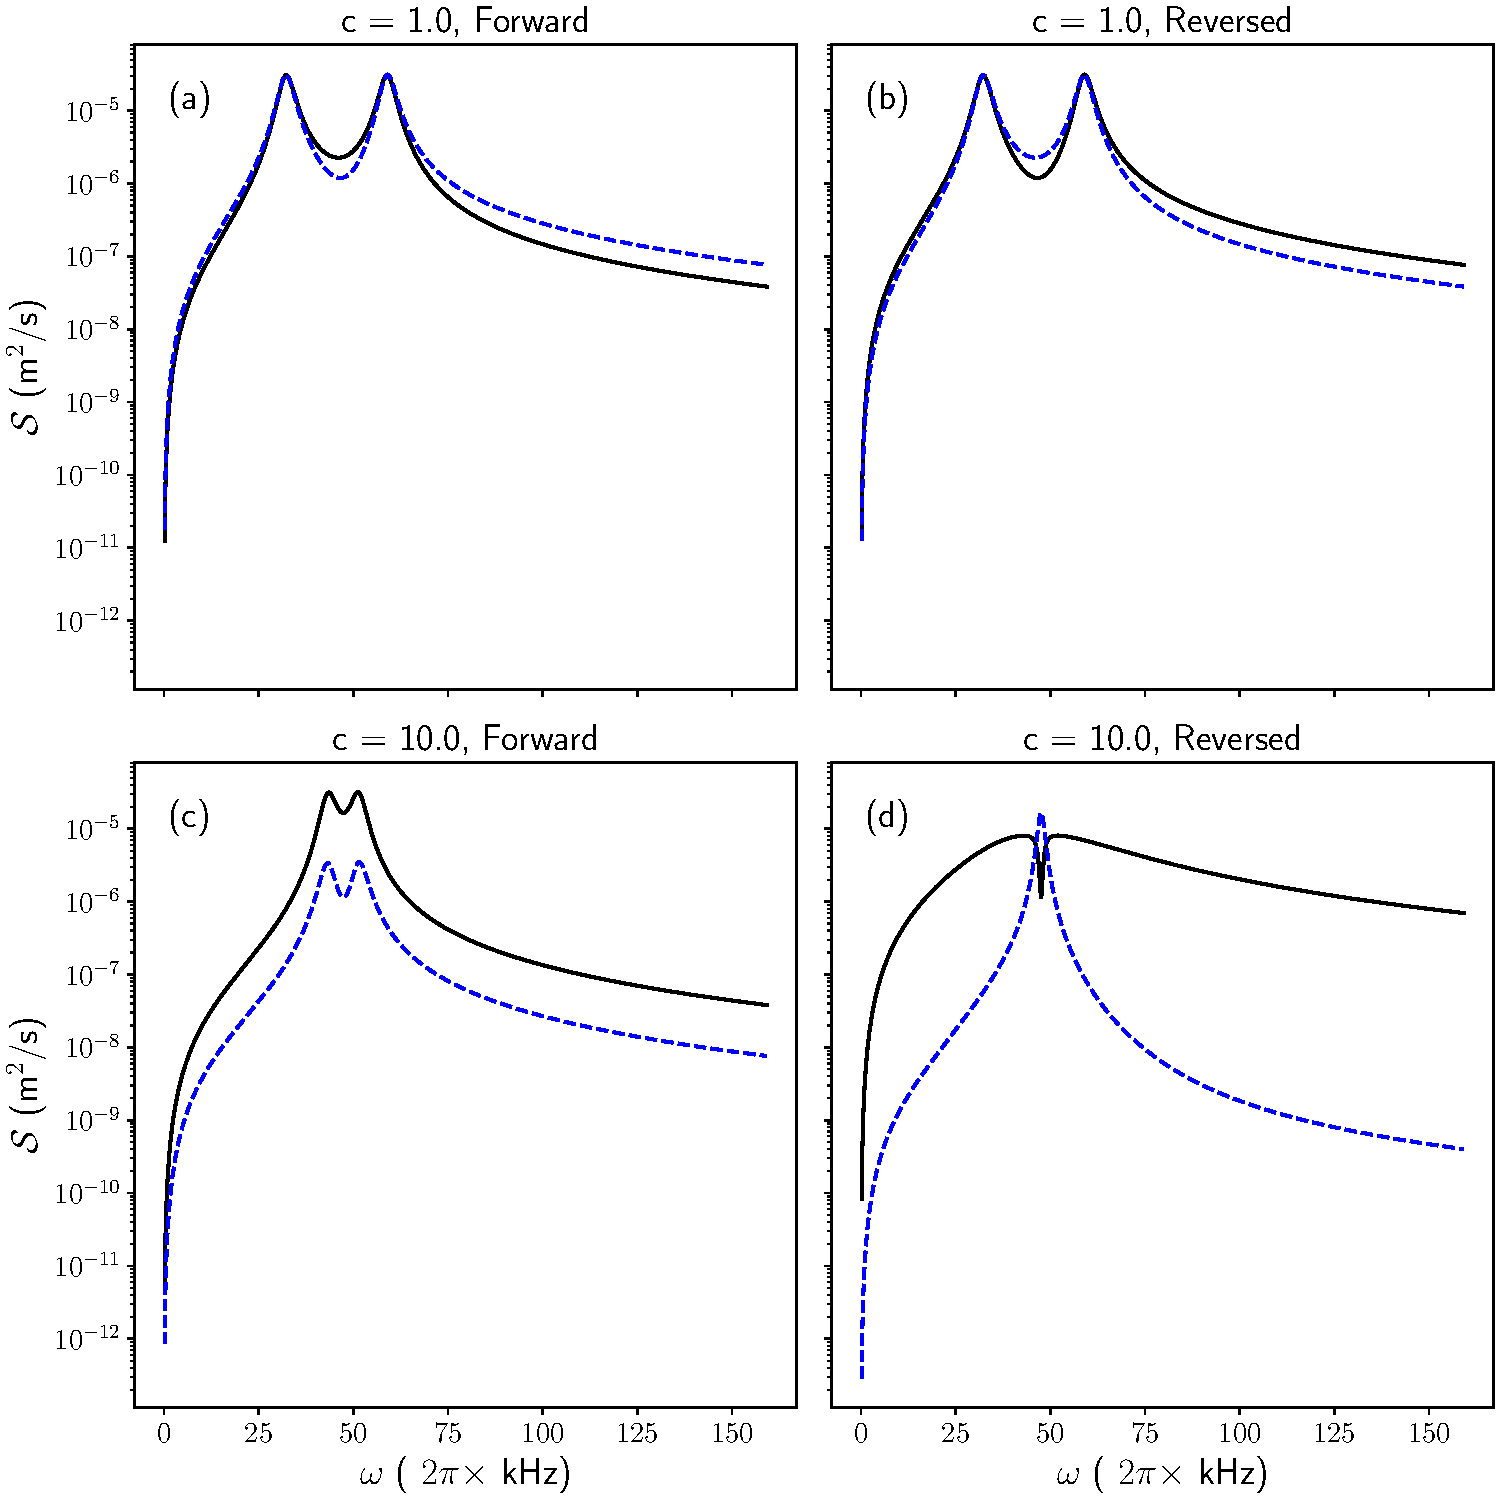
\includegraphics[width=\linewidth]{Figures/SpectrumComparative.pdf}
  \caption{Spectral densities of the velocities of the ions ($r_3$ and $r_4$) corresponding to different values of $c$ in Fig. \ref{fig:Fig_PerfectRectification}: (a), (b) for $c=1$ and (c), (d) for $c=10$. Solid, black lines correspond to the left ion velocity spectral density $\mathbb{S}_{3,3}(\omega)$ and dashed, blue lines correspond to the right ion velocity spectral density $\mathbb{S}_{4,4}(\omega)$. (a) and (b) correspond to $R = 0$:  the overlap between the phonon bands is the same in the forward and reversed configurations. (c) and (d) correspond to $R\approx 0.8$:  in the forward configuration (c)  the phonons match better than in the reversed configuration (d).}
  \label{fig:Figure_Spectra}
\end{figure}


For the vector process $\overrightarrow{r}(t)$ describing the evolution of our system we have $\overrightarrow{R}(\omega) = \left( i \omega - \mathbb{A} \right)^{-1}\mathbb{L}\overrightarrow{\Xi}(\omega)$ with $\overrightarrow{\Xi}(\omega)$ being the Fourier transform of the white noise $\overrightarrow{\xi}(t)$. Note that $\overrightarrow{\Xi}(\omega)$ does not strictly exist, because it is not square-integrable, however its spectral density is $\mathbb{S}_{\overrightarrow{\xi}}(\omega) = 2 \mathbb{D}$ \cite{Sarkka2019}, which is flat as expected for a white noise. Therefore, the spectral density matrix of the system is
%
\begin{equation}
  \mathbb{S}_{\overrightarrow{r}} = 2 \left(  \mathbb{A} - i\omega\right)^{-1}\mathbb{L}\mathbb{D}\mathbb{L}^\mathsf{T}\left(  \mathbb{A} + i\omega\right)^{-\mathsf{T}}.
  \label{eq:SpectralDensityToyModelB}
\end{equation}
%
As we can see in Eq. \eqref{eq:SpectralDensityToyModelB}, the imaginary part of the eigenvalues of the dynamical matrix $\mathbb{A}$ correspond to the peaks in the spectrum whereas the real part dictates their width. The spectral density matrix of our model is
%
\begin{equation}
  \mathbb{S}_{\overrightarrow{r}}(\omega) = 2 k_B \frac{\gamma_L T_L\mathbb{S}_L(i\omega)+\gamma_L T_R\mathbb{S}_R(i\omega)}{(m_1 m_2)^2 P_\mathbb{A}(i\omega)P_\mathbb{A}(-i\omega)},
\end{equation}
%
where $P_\mathbb{A}(\lambda)$ is the characteristic polynomial of the dynamical matrix $\mathbb{A}$ and $\mathbb{S}_L(\omega)$, $\mathbb{S}_R(\omega)$ are the matrix polynomials in the angular frequency $\omega$ whose coefficients are defined in Appendix \ref{Appendix:SpectralDensity}. Equation \eqref{eq:SpectralDensitiesVelocities} gives the full expressions of the spectral densities for the velocities, $\mathbb{S}_{3,3}(\omega) = \expval{R_3(\omega)R_3(-\omega)}$ for the left ion, and $\mathbb{S}_{4,4}(\omega) = \expval{R_4(\omega)R_4(-\omega)}$ for the right ion, since they are the elements related to the calculation of the heat current using Eq. \eqref{eq:Wiener-Khinchin},
%
\begin{align}
  \mathbb{S}_{3,3}(\omega) &= 2 k_B \frac{\gamma_R k^2 T_R \omega ^2+\gamma_L T_L \left[\omega ^4 \left(\gamma_R^2-2 k m_2-2 k_R m_2\right)+\omega ^2 (k+k_R)^2+m_2^2 \omega ^6\right]}{(m_1 m_2)^2 P_\mathbb{A}(i\omega)P_\mathbb{A}(-i\omega)},\nonumber\\
  %
%    \nonumber\\
  %
  \mathbb{S}_{4,4}(\omega) &= 2 k_B \frac{\gamma_L k^2 T_L \omega ^2+\gamma_R T_R \left[\omega ^4 \left(\gamma_L^2-2 k m_1-2 k_L m_1\right)+\omega ^2 (k+k_L)^2+m_1^2 \omega ^6\right]}{(m_1 m_2)^2 P_\mathbb{A}(i\omega)P_\mathbb{A}(-i\omega)}.
  \label{eq:SpectralDensitiesVelocities}
\end{align}
%
Figure \ref{fig:Figure_Spectra} depicts a series of plots of the spectra given by Eq. \eqref{eq:SpectralDensitiesVelocities} that correspond to two points in Fig. \ref{fig:Fig_PerfectRectification}. For $c=1$ (Fig. \ref{fig:Figure_Spectra}(a) and (b)) there is no rectification, since the spectra match in the forward (a) and reversed (b) configurations. However, for $c=10$ ((Fig. \ref{fig:Figure_Spectra}(c) and (d))) the picture is very different: there is a good match between the spectra in the forward configuration whereas in the reversed configuration the spectra are less correlated, giving as a result higher rectification ($R \approx 0.8$). Figure \ref{fig:Figure_Spectra} only shows the elements (3,3) and (4,4) in the diagonal of $\mathbb{S}$ but the remaining elements, including off-diagonal ones, exhibit a similar behavior.
% with respect to rectification.
%
\section{Conclusions \label{sec:Conclusions}}
%
We have studied heat rectification in a model composed of two coupled harmonic oscillators connected to baths. This simple model allows analytical treatment but still has enough complexity to examine different ingredients that can produce rectification. %We have also derived analytical expressions for the heat currents and local temperatures.
Our results demonstrate in a simple but realistic system that harmonic systems can rectificate heat current if they have features which depend on the temperature  \cite{Pereira2017}. We implement this notion of temperature-dependent features by defining the baths exchange operation as an exchange of both temperatures and coupling parameters of the baths to the system. This kind of temperature-dependent features happens naturally in laser-cooled trapped ion set-ups.

We have also studied the phonon spectra of the system, comparing the match/mismatch of the phonon bands, to reach the conclusion that the band match/mismatch description for heat rectification is also valid for systems which are harmonic, as long as there are temperature-dependent features.
We hope this article sheds more light into the topic of heat rectification and that encourages more research regarding its physical implementation on chains of trapped ions.
 %Rectification Toy Model

%!TEX root = ../Thesis.tex
%Conclusions Chapter

% \chapter*{Conclusions}
\label{Conclusions}
\lhead{\emph{Conclusions}}
\null
% \vfill
\textit{``Don't adventures ever have an end? I suppose not. Someone else always has to carry on the story.''}
\begin{flushright}
  {\bf J. R. R. Tolkien}\\
  The Fellowship of the Ring
\end{flushright}
%\vfill
\null

In this Thesis I have presented the most relevant results of the research I have conducted during my PhD, which embraces the study of asymmetric scattering and heat transport. The general goal of my research was to design devices that alow asymmetric transport and that are reallistic enough, so they can be implemented experimemtally. In this chapter I will summarize in a few pages the main results of this Thesis and present my conclusions.

Since this Thesis is divided in a first part, which adresses the design of asymmetric devices based on non-Hermitian and non-local potentials, and a second part, which focus on the design of thermal rectifiers, I will present the conclusions to each part in different sections.
% Finally, I shall present my general conclusions for the entirety of my work.


\section*{Conclusions to part I}

\begin{itemize}
  \item {\bf Asymmetric scattering by non-Hermitian potentials}
  \begin{itemize}
    \item Six types of devices with asymmetric scattering are possible when imposing 0 or 1 for the values of the scattering probabilities.

    \item Hermitian Hamiltonians do not allow for any asymmetry in transmission and
    reflection probabilities, therefore in order to design asymmetric devices non-hermitian
    Hamiltonians are needed. Besides, non-local potentials are needed for asymmetric scattering.

    \item There are 8 symmetries that generate all the possible transformations of the potential matrix elements, which consist in complex conjugation, coordinate inversion, the identity and transposition. The eight symmetries arise from the commutation or pseudohermiticity of the potential with an element of the Klein’s 4-group $\mathbb{K}_4 = \{1,\Pi,\Theta,\Pi\theta\}$. The symmetries impose selection rules for the scattering amplitudes that conditions the design of some of the devices.

    \item The conventional definition of a symmetry in terms of commutation with a unitary/antiunitary operator $A$ is extended with the concept of $A$-pseudohermiticity for non-Hermitian Hamiltonians. Both commutation and $A$-pseudohermiticity must be considered on the same footing.

    \item Some example potentials are given for the different asymmetric devices, in particular a local PT-potential that works as transparent 1-way reflector in a broad domain of incident momenta.

  \end{itemize}

  \item {\bf $S$-matrix pole symmetries for non-Hermitian scattering Hamiltonians}
  \begin{itemize}
    \item The symmetries of a non-Hermitian Hamiltonian, understood as commutation or $A$-pseudohermiticity, can be rewritten as the invariance of $H$ with respect to the action of a unitary or antiunitary superoperator, $H = \mathcal{L}(H)$. Following this approach with the 8 symmetries described in chapter \ref{Chapter1} a group structure is unveiled: the 8 symmetries form the elementary abelian group E8.

    \item In refs. \cite{Mostafazadeh2002,Mostafazadeh2002a,Mostafazadeh2002b} it was shown that
    $A$-pseudohermiticity, with $A$ linear and hermitian, or commutavity with an antilinear hermitian operator were necessary and sufficient conditions for a discrete Hamiltonian to have conjugate pairs of discrete eigenenergies. I show that this result can be extended to scattering Hamiltonians. Scattering Hamiltonians that satisfy the same conditions, have the poles of their $S$-matrix forming conjugate pairs in the complex energy plane.

    \item I provided examples of the distribution of poles using separable potentials. The two examples correspond to the non-trivial symmetries: time-reversal and parity-pseudohermicity.

  \end{itemize}

  \item {\bf Quantum-optical implementation of non-Hermitian potentials for asymmetric scattering}
  \begin{itemize}
    \item I propose a quantum-optical implementation of non-local and non-Hermitian potentials
    with asymmetric scattering amplitudes. Since they are non-local and also non-PT symmetrical they allow asymmetric transmission.

    \item The non-Hermitian potentials are constructed by obtaining the effective dynamics for the ground state of a two-level atom impinging on a laser field. This is done using Feshbach projection technique.

    \item I present examples of a $\mathcal{T/A}$ device (One-way T-filter), a $\mathcal{R/A}$ device (One-way R-filter) and a partial $\mathcal{TR/A}$ device (One-way mirror).

  \end{itemize}

\end{itemize}

\section*{Conclusions to part II}

\begin{itemize}
  \item {\bf Local rectification of heat flux}
  \begin{itemize}
    \item I have presented a design for a thermal rectifier based on a localized impurity in a chain of atoms. The on-site potential and interatomic interactions are modeled with harmonic and Morse potentials, respectively.

    \item As oposed to other models, the chain is homogeneous and the only structural asymmetry is only in the impurity.

    \item The numerical results show normal heat conduction in the absence of the impurity and rectification when it is present.

    \item Rectification is also present when the Morse interaction is substituted by a harmonic one, although it is slightly fainter

  \end{itemize}

  \item {\bf Asymmetric heat transport in ion crystals}
  \begin{itemize}
    \item I introduced a model of a chain of ions trapped in individual microtraps and in contact at both ends with thermal baths mediated by optical molasses.

    \item Numerical results show that there is rectification when the microtrap frequencies are graded along the chain.

    \item In this model I explore some of the mechanisms that have been proposed in the literature to improve rectification, namely long range interactions and graded structures.

    \item This model could be implemented in a trapped-ion platform, which is interesting because is one of the most controllable quantum technologies platform. Besides, this work connects two different scientific communities: ion trappers and researchers in thermal rectification.
  \end{itemize}

  \item {\bf Heat rectification with a minimal model of two harmonic oscillators}
  \begin{itemize}
    \item  I study thermal rectification in an analytically treatable model
    composed of two coupled harmonic oscillators connected to Langevin Baths.

    \item The results demonstrate that thermal rectification is even possible in
    harmonic systems if there are temperature-dependent features. In this case, the
    temperature dependence is in the coupling of the oscillators to the baths. This
    temperature dependence arise naturally in Doppler-cooled trapped-ion setups.

    \item The phonon band match-mismatch description that was proposed for non-harmonic
    systems also applies in this harmonic model.
  \end{itemize}

\end{itemize}

% \section*{General conclusions}
 %Conclusions
\addcontentsline{toc}{chapter}{Conclusions}

%% ----------------------------------------------------------------
% Now begin the Appendices, including them as separate files

\addtocontents{toc}{\vspace{2em}} % Add a gap in the Contents, for aestheticsy

\appendix % Cue to tell LaTeX that the following 'chapters' are Appendices
\part*{Appendix}
%\addcontentsline{toc}{part}{Appendix}
\addtocontents{toc}{\vspace{0.6em}}

%!TEX root = ../Thesis.tex
% Appendix A

\chapter{Interaction versus asymmetry for adiabatic following}
\label{Interaction versus asymmetry for adiabatic following}
\lhead{Appendix A. \emph{Interaction versus asymmetry for adiabatic following}}

%

Extra information to add to your thesis.
	% Interaction versus asymmetry for adiabatic following

\addtocontents{toc}{\vspace{0.6em}}  % Add a gap in the Contents, for aesthetics
\backmatter
\pagestyle{empty}  % Page style needs to be empty for this page

%% ----------------------------------------------------------------
\label{Bibliography}
\lhead{\emph{Bibliography}}  % Change the left side page header to "Bibliography"
%\bibliographystyle{apsrev}  % Use the "unsrtnat" BibTeX style for formatting the Bibliography
%\bibliographystyle{h-physrev3} % formato PRA sin url ni issn ni hyperlinks
\bibliographystyle{sofia} %modificado por mi a partir de utphys
%\bibliographystyle{utphys} %formato arXiv con hyperlinks
\bibliography{Bibliography_Thesis}  % The references (bibliography) information are stored in the file named "Bibliography_Thesis.bib"

\end{document}  % The End
%% ----------------------------------------------------------------
